%% abtex2-modelo-trabalho-academico.tex, v-1.9.1 laurocesar
%% Copyright 2012-2013 by abnTeX2 group at http://abntex2.googlecode.com/ 
%%
%% This work may be distributed and/or modified under the
%% conditions of the LaTeX Project Public License, either version 1.3
%% of this license or (at your option) any later version.
%% The latest version of this license is in
%%   http://www.latex-project.org/lppl.txt
%% and version 1.3 or later is part of all distributions of LaTeX
%% version 2005/12/01 or later.
%%
%% This work has the LPPL maintenance status `maintained'.
%% 
%% The Current Maintainer of this work is the abnTeX2 team, led
%% by Lauro César Araujo. Further information are available on 
%% http://abntex2.googlecode.com/
%%
%% This work consists of the files abntex2-modelo-trabalho-academico.tex,
%% abntex2-modelo-include-comandos and abntex2-modelo-references.bib
%%

% ------------------------------------------------------------------------
% ------------------------------------------------------------------------
% abnTeXf2: Modelo de Trabalho Academico (tese de doutorado, dissertacao de
% mestrado e trabalhos monograficos em geral) em conformidade com 
% ABNT NBR 14724:2011: Informacao e documentacao - Trabalhos academicos -
% Apresentacao
% ------------------------------------------------------------------------
% ------------------------------------------------------------------------

\documentclass[
	% -- opções da classe memoir --
	12pt,				% tamanho da fonte
	openany,			% capítulos começam em qualquer página (para iniciar em página ímpar, tente openright)
	twoside,			% para impressão em páginas corretamente
	a4paper,			% tamanho do papel. 
	% -- opções da classe abntex2 --
	%chapter=TITLE,		% títulos de capítulos convertidos em letras maiúsculas
	%section=TITLE,		% títulos de seções convertidos em letras maiúsculas
	%subsection=TITLE,	% títulos de subseções convertidos em letras maiúsculas
	%subsubsection=TITLE,% títulos de subsubseções convertidos em letras maiúsculas
	% -- opções do pacote babel --
	english,			% idioma adicional para hifenização
	french,				% idioma adicional para hifenização
	spanish,			% idioma adicional para hifenização
	brazil,				% o último idioma é o principal do documento
	oldfontcommands
	]{abntex2}

% ---
% Pacotes básicos 
% ---
\usepackage{lmodern}			% Usa a fonte Latin Modern			
\usepackage[T1]{fontenc}		% Selecao de codigos de fonte.
\usepackage[utf8]{inputenc}		% Codificacao do documento (conversão automática dos acentos)
\usepackage{lastpage}			% Usado pela Ficha catalográfica
\usepackage{indentfirst}		% Indenta o primeiro parágrafo de cada seção.
\usepackage{color}				% Controle das cores
\usepackage{graphicx}			% Inclusão de gráficos
\usepackage{microtype} 			% Melhorias de justificação
\usepackage{pdfpages}			% Inserir páginas de pdf
\usepackage{amsmath}			% Funções Matemáticas
\usepackage{epstopdf}
% ---
		
% ---
% Pacotes adicionais, usados apenas no âmbito do Modelo Canônico do abnteX2
% ---
\usepackage{lipsum}				% para geração de dummy text
% ---

% ---
% Pacotes de citações
% ---
\usepackage[brazilian,hyperpageref]{backref}
% Paginas com as citações na bibl
\usepackage[num]{abntex2cite}	% Citações padrão ABNT

% --- 
% CONFIGURAÇÕES DE PACOTES
% --- 

% ---
% Configurações do pacote backref
% Usado sem a opção hyperpageref de backref
\renewcommand{\backrefpagesname}{Citado na(s) página(s):~}
% Texto padrão antes do número das páginas
\renewcommand{\backref}{}
% Define os textos da citação
\renewcommand*{\backrefalt}[4]{
	\ifcase #1 %
		Nenhuma citação no texto.%
	\or
		Citado na página #2.%
	\else
		Citado #1 vezes nas páginas #2.%
	\fi}%
% ---

% ---
% Informações de dados para CAPA e FOLHA DE ROSTO
% ---
\titulo{Sistema de controle de atitude para satélite CubeSat}
\autor{Augusto Bonangelo Costa\\
Felipe Ramos de Faria\\
William Mazi}
\local{São Caetano do Sul}
\data{2015}
\orientador{Prof. Dr. Rodrigo Alvite Romano}
%\coorientador{Professor}
\instituicao{Escola de Engenharia Mauá do Centro Universitário do Instituto Mauá de Tecnologia}
\tipotrabalho{Trabalho de Conclusão de Curso de Engenharia de Controle e Automação}
% O preambulo deve conter o tipo do trabalho, o objetivo, 
% o nome da instituição e a área de concentração 
\preambulo{Trabalho de Conclusão de Curso apresentado à Escola de Engenharia Mauá do Centro Universitário do Instituto Mauá de Tecnologia como requisito parcial para a obtenção do título de Engenheiro de Controle e Automação.}
% ---

% ---
% Configurações de aparência do PDF final

% alterando o aspecto da cor azul
\definecolor{blue}{RGB}{41,5,195}

% informações do PDF
\makeatletter
\hypersetup{
     	%pagebackref=true,
		pdftitle={\@title}, 
		pdfauthor={\@author},
    	pdfsubject={\imprimirpreambulo},
	    pdfcreator={LaTeX with abnTeX2},
		pdfkeywords={abnt}{latex}{abntex}{abntex2}{trabalho acadêmico}, 
		colorlinks=true,       		% false: boxed links; true: colored links
    	linkcolor=black,          	% color of internal links
    	citecolor=black,        	% color of links to bibliography
    	filecolor=black,      		% color of file links
		urlcolor=black,
		bookmarksdepth=4 
}
\makeatother
% --- 

% --- 
% Espaçamentos entre linhas e parágrafos 
% --- 

% O tamanho do parágrafo é dado por:
\setlength{\parindent}{1.25cm}

% Controle do espaçamento entre um parágrafo e outro:
\setlength{\parskip}{0.2cm}  % tente também \onelineskip

% ---
% compila o indice
% ---
\makeindex
% ---

% ----
% Início do documento
% ----
\begin{document}

% Retira espaço extra obsoleto entre as frases.
\frenchspacing

% ----------------------------------------------------------
% ELEMENTOS PRÉ-TEXTUAIS
% ----------------------------------------------------------
% \pretextual

% ---
% Capa
% ---
\imprimircapa
% ---

% ---
% Folha de rosto
% (o * indica que haverá a ficha bibliográfica)
% ---
\imprimirfolhaderosto*
% ---

% ---
% Inserir a ficha bibliografica
% ---

% Isto é um exemplo de Ficha Catalográfica, ou ``Dados internacionais de
% catalogação-na-publicação''. Você pode utilizar este modelo como referência. 
% Porém, provavelmente a biblioteca da sua universidade lhe fornecerá um PDF
% com a ficha catalográfica definitiva após a defesa do trabalho. Quando estiver
% com o documento, salve-o como PDF no diretório do seu projeto e substitua todo
% o conteúdo de implementação deste arquivo pelo comando abaixo:
%
% \begin{fichacatalografica}
%     \includepdf{fig_ficha_catalografica.pdf}
% \end{fichacatalografica}
\begin{fichacatalografica}
	\vspace*{\fill}					% Posição vertical
	\hrule							% Linha horizontal
	\begin{center}					% Minipage Centralizado
	\begin{minipage}[c]{12.5cm}		% Largura
	
	Costa, Augusto Bonangelo Costa
	
	\hspace{0.5cm} \imprimirtitulo  / Augusto Bonangelo Costa, Felipe Ramos de Faria, William Mazi. --
	\imprimirlocal, CEUN-IMT, \imprimirdata
	
	\hspace{0.5cm} \pageref{LastPage} p.\\
	
	\hspace{0.5cm}
	\parbox[t]{\textwidth}{\imprimirtipotrabalho~--~\imprimirinstituicao,
	\imprimirlocal, \imprimirdata.}\\
	
	\hspace{0.5cm} \imprimirorientadorRotulo~\imprimirorientador\\
	
	\hspace{0.5cm}
		1. Controle de Atitude.
		2. CubeSat.
		I. Faria, Felipe Ramos de
		II. Mazi, William
		III. Instituto Mauá de Tecnologia. Centro Universitário. Escola de Engenharia Mauá.
		IV. Título\\ 			
	
%	\hspace{8.75cm} CDU \\
	
	\end{minipage}
	\end{center}
	\hrule
\end{fichacatalografica}
% ---

% ---
% Inserir folha de aprovação
% ---

% Isto é um exemplo de Folha de aprovação, elemento obrigatório da NBR
% 14724/2011 (seção 4.2.1.3). Você pode utilizar este modelo até a aprovação
% do trabalho. Após isso, substitua todo o conteúdo deste arquivo por uma
% imagem da página assinada pela banca com o comando abaixo:
%
% \includepdf{folhadeaprovacao_final.pdf}
%
\begin{folhadeaprovacao}

  \begin{center}
    {\ABNTEXchapterfont\large\imprimirautor}

    \vspace*{\fill}\vspace*{\fill}
    \begin{center}
      \ABNTEXchapterfont\bfseries\Large\imprimirtitulo
    \end{center}
    \vspace*{\fill}
    
    \hspace{.45\textwidth}
    \begin{minipage}{.5\textwidth}
    \end{minipage}%
    \vspace*{\fill}
   \end{center}
        
Trabalho de Conclusão de Curso aprovado em \_\_\_ de \_\_\_\_\_\_\_\_\_\_\_\_\_ de 2015, pela banca examinadora composta por: 

   \assinatura{\textbf{\imprimirorientador} \\ Orientador} 
   \assinatura{\textbf{Professor} \\ Convidado 1}
   \assinatura{\textbf{Professor} \\ Convidado 2}
   %\assinatura{\textbf{Professor} \\ Convidado 3}
   %\assinatura{\textbf{Professor} \\ Convidado 4}
      
   \begin{center}
    \vspace*{0.5cm}
    {\large\imprimirlocal}
    \par
    {\large\imprimirdata}
    \vspace*{1cm}
  \end{center}
  
\end{folhadeaprovacao}
% ---

% ---
% Dedicatória
% ---

% ---
% Agradecimentos
% ---
\begin{agradecimentos}

A Escola de Engenharia Mauá por fornecer toda a gama de conhecimento e estrutura para um melhor aprendizado.\par

Ao {\imprimirorientador}  pela assessoria prestada quanto ao desenvolvimento do tema.\par

Ao Prof. Rafael Corsi por todo empenho dedicado auxiliando o projeto de distintas maneiras.\par

Ao técnico Fernando Nery Bueno por toda ajuda prestada durante diversas etapas do projeto.\par

E aos nossos pais, amigos e namoradas que apesar de todas as dificuldades sempre nos suportaram para o melhor desenvolvimento do projeto.

\end{agradecimentos}
% ---

% ---
% Epígrafe
% ---
\begin{epigrafe}
    \vspace*{\fill}
	\begin{flushright}
		\textit{Tudo aquilo que o homem ignora não existe para ele. Por isso o universo de cada um se resume ao tamanho de seu saber.\\(Albert Einstein)}
	\end{flushright}
\end{epigrafe}
% ---

% ---
% RESUMOS
% ---
% resumo em português
\setlength{\absparsep}{18pt} % ajusta o espaçamento dos parágrafos do resumo
\begin{resumo}
 Resumo do TCC

 \textbf{Palavras-chaves}: CubeSat, Controle de atitude, Satélite, Roda de reação, Sistemas embarcados.
\end{resumo}

% resumo em inglês
\begin{resumo}[Abstract]
 \begin{otherlanguage*}{english}
   This is the english abstract.

   \vspace{\onelineskip}
 
   \noindent 
   \textbf{Key-words}: CubeSat, Attitude control, Satellite, Reaction wheel, Embedded systems.
 \end{otherlanguage*}
\end{resumo}

% ---
% inserir lista de ilustrações
% ---
\pdfbookmark[0]{\listfigurename}{lof}
\listoffigures*
\cleardoublepage

% ---
% inserir lista de tabelas
% ---
\pdfbookmark[0]{\listtablename}{lot}
\listoftables*
\cleardoublepage

% ---
% inserir lista de abreviaturas e siglas
% ---
\begin{siglas}

  \item[AEB] {Agência Espacial Brasileira}
  \item[ADC] {Conversor Analógico-Digita}
  \item[BLDC] \textit{Brushless Direct Current Motor}
  \item[Cal Poly] \textit{California Polytechnic State University}
  \item[COTS] \textit{Commercial Off-The-Shelf}
  \item[CubeSat] \textit{Cube-Satellite}
  \item[DSP] \textit{Digital Signal Processing}
  \item[ESA] \textit{European Space Agency}
  \item[I$^{2}$C] \textit{Inter-Integrated Circuit}
  \item[IMT] {Instituto Mauá de Tecnologia}
  \item[IMU] \textit{Inercial Measurement Unit}
  \item[INPE] {Instituto Nacional de Pesquisas Espaciais}
  \item[ISS] \textit{International Space Station}
  \item[MIPS] {Milhões de Instruções Por Segundo}
  \item[NSA] \textit{National Aeronautics and Space Administration}
  \item[NSEE] {Núcleo de Sistemas Eletrônicos Embarcados}
  \item[U] \textit{Unit}
  \item[PI] {Proporcional-Integral}
  \item[PIC] \textit{Programmable Interface Controller}
  \item[PWM] \textit{Pulse-Width Modulation}
    
\end{siglas}

% ---
% inserir lista de símbolos
% ---
%\begin{simbolos}
%  \item[$ \Gamma $] Letra grega Gama
%  \item[$ \Lambda $] Lambda
%  \item[$ \zeta $] Letra grega minúscula zeta
%  \item[$ \in $] Pertence
%\end{simbolos}

% ---
% inserir o sumario
% ---
\pdfbookmark[0]{\contentsname}{toc}
\tableofcontents*
\cleardoublepage

% ----------------------------------------------------------
% ELEMENTOS TEXTUAIS
% ----------------------------------------------------------
\textual

% ----------------------------------------------------------
% Introdução (exemplo de capítulo sem numeração, mas presente no Sumário)
% ----------------------------------------------------------
\chapter{Introdução}

CubeSats (\textit{Cube-Satellite}) são satélites que possuem forma de cubo com aresta de 100mm e massa de até 1330g. Essas definições correspondem a uma unidade de CubeSat, que é representada pela sigla U (\textit{Unit}). É comum a utilização dessas unidades em conjuntos de 2U (200x100x100mm), 3U (300x100x100) ou 6U (300x200x100) \cite{NASA}. É utilizado como plataforma para realização de experimentos por instituições de ensino e pesquisa além de empresas que buscam uma solução de baixo custo para o desenvolvimento de novas tecnologias. O motivo pelo qual são necessárias pequenas quantias de investimentos é a utilização de materiais comerciais de prateleira (\textit{commercial off-the-shelf} - COTS), ou seja, materiais que podem ser encontrados no comércio, e de possuir um design padronizado que reduz tempo e custo de desenvolvimento \cite{CalPoly}.

Um dos principais sistemas dos satélites é o sistema de determinação e controle de atitude. A atitude é a orientação de um corpo em relação a uma referência externa em um dado sistema de coordenadas. O sistema de determinação e controle de atitude é composto por duas etapas principais: determinação de atitude e controle de atitude \cite{FrancLav}.

A determinação de atitude é o processo que envolve a aquisição de dados através de sensores de posicionamento que indicam para o sistema de controle de atitude qual a posição do satélite em relação a um referencial fixo \cite{FrancLav}. Esse processo possui elevada complexidade e, como não é objeto desse estudo, não será abordado com muita profundidade.

O controle de atitude é a atuação do sistema que movimentará o satélite, mudando sua posição em relação a um referencial. Em geral, o que define qual método de controle de atitude é empregado são a precisão do apontamento, a estabilidade, e a capacidade de manobra. Outros fatores também influenciam como custo, peso, confiabilidade, movimento orbital e vida útil. As várias formas de executar esse controle podem ser agrupadas em controle passivo ou controle ativo, de acordo com o tipo de torque \cite{FrancLav}.

O controle passivo pode ser feito de duas maneiras, por gradiente de gravidade, onde o eixo mais longo do satélite aponta para a Terra, mantendo assim uma orientação fixa em relação a mesma. Outro modo de controle passivo é através do alinhamento de um imã no satélite com as linhas de campo magnético da terra \cite{FrancLav}.

Já o controle ativo é feito de três formas principais. Uma delas consiste em manter o satélite girando em torno do eixo que aponta na direção desejada. Outro método é através de propulsores que geram impulso para a movimentação do satélite. Há ainda a manipulação de cada um dos ângulos de Euler (\textit{Roll-Pitch-Yaw}), o qual garante maior precisão no seu apontamento e facilita seu uso para experimentos científicos ou telecomunicações \cite{FrancLav}. Para este tipo de controle, os acionadores mais utilizados são as rodas de reação, os magnetorquers e os jatos de gás.

% ----------------------------------------------------------
% Justificativa
% ----------------------------------------------------------
\section{Justificativa}

	A área aeroespacial é importante para todo país que possui desenvolvimento tecnológico. A causa disso é a ajuda em desenvolver outras áreas paralelamente. Porém, desenvolvimentos de satélites são caros e o CubeSat entra como alternativa de baixo custo e acessível tanto a instituições de ensino quanto a empresas interessadas no setor \cite{DIY}.
	
Outro ponto positivo são as diversas aplicações que se dão a satélites, inclusive os do tipo CubeSat. Um exemplo é a pesquisa da "Anomalia do Atlântico Sul". Esta anomalia ocorre porque o campo magnético da Terra é mais fraco exatamente sobre a América do Sul e boa parte do Oceano Atlântico Sul, permitindo ondas magnéticas solares penetrarem mais fundo na atmosfera terrestre nesse ponto, causando interferência em satélites \cite{MORAES}. Um satélite do tipo CubeSat poderia ser usado para levantar mais dados a respeito desse fenômeno, através de medições diretas ou fotografias. Outro exemplo é utilizar o CubeSat para expor microrganismos ao ambiente espacial e analisar como se desenvolvem.

Além de todos estes motivos, um grande incentivo é nos iniciar na área espacial. Este estudo nos serve de base para aprender um pouco sobre soluções usando sistemas embarcados, sistemas de controle e diversas outras aplicações que nos podem ser úteis em nossas vidas profissionais, quaisquer que sejam nossas áreas de atuação.

% ----------------------------------------------------------
% Objetivo
% ----------------------------------------------------------
\section{Objetivos}

O objetivo deste estudo é projetar e construir o sistema de controle de atitude para um satélite do tipo CubeSat.

Este estudo servirá de base para o desenvolvimento de futuros CubeSats com melhores desempenhos e abrirá a possibilidade de que um deles possa ser enviado ao espaço com o objetivo de cumprir ou ajudar em alguma missão espacial.

\subsection{Objetivos primários}

Alguns dos principais objetivos deste trabalho são:

a)	modelagem e validação de sistemas;

b)	aprendizagem sobre rodas de reação;

c)	aprendizagem sobre softwares de projeto de placas de circuitos micro eletrônicos;

d)	aprendizagem sobre protocolo de comunicação I$^{2}$C;

e)	testes e validações do sistema de controle em um e mais graus de liberdade;

f) validação do motor \textit{brushless}.

% ----------------------------------------------------------
% Revisão bibliográfica
% ----------------------------------------------------------

\chapter{Revisão bibliográfica}

Como um guia para o trabalho, foi feito uma pesquisa bibliográfica sobre a qual o trabalho se baseou. Esta etapa da pesquisa tornou possível observar quem são os países que desenvolvem CubeSats, como é utilizado ao redor do mundo e como o Brasil está em relação aos desenvolvedores desta tecnologia, além de compreende as duas etapas que envolvem o módulo de atitude de um CubeSat, a determinação de atitude e o controle de atitude.

\section{Origem}

A concepção do CubeSat teve início no ano de 1999 através de um esforço em conjunto da Stanford University e California Polytechnic State University, que criaram as primeiras especificações que serviram de base para aos atuais CubeSats. O objetivo era possibilitar que estudantes pudessem projetar, construir, testar e operar um satélite com funcionalidades parecidas com as do Sputnik I, que eram emitir um sinal constante para a Terra, e medir a densidade da atmosfera \cite{SmallSat}.

\section{CubeSat no mundo} 

A maioria dos CubeSats lançados até hoje foram projetados, desenvolvidos e construídos nas universidades norte-americanas, como o XSAS, desenvolvido pela \textit{University of Michigan} \cite{MCKAY}, o \textit{Vermont Lunar CubeSat}, desenvolvido pela \textit{Vermont Technical College} \cite{Vermont}, além de outros desenvolvidos pelas veteranas \textit{Stanford University} \cite{TWIGGS} e \textit{California Polytechnic State University} \cite{PolySat}.

Algumas empresas privadas já desenvolveram seus próprios CubeSats, como é o caso da Boeing \cite{Boeing}. Eles desenvolveram um CubeSat com o objetivo de desenvolver sistemas de controle de atitude que seriam usados para refinar os sistemas usados nos aviões produzidos pela empresa.

Há ainda o caso da Planet Labs \cite{PlanetLabs}, empresa que desenvolveu e fabricou 28 CubeSats (de nome Dove) dotados de uma câmera fotográfica de alta resolução. Todos foram lançados ao espaço formando um conjunto chamado de Dove. Esse conjunto está espalhado pelo mundo. A Planet Labs vende o serviço fotográfico desses satélites. Sempre que alguém contrata esse serviço, eles tiram fotos do local especificado pela pessoa por um período. Esse serviço pode ser usado empresas de mineração, exploração de recursos naturais, monitoramento agrícola, monitoramento de desmatamento, etc. Isso mostra o quão abrangente são as possibilidades de uso dos CubeSats.

Diversos outros países já fizeram e lançaram ao menos um protótipo, como a Dinamarca, com o AAUSAT4, desenvolvido pela \textit{Aalborg University} \cite{AAUSAT}, o Canada, com o CANX-2, desenvolvido pela \textit{University of Toronto} \cite{CANX} e o Japão, com o CUTE 1, desenvolvido pela \textit{Tokyo Institute of Technology} \cite{CUTE}. Alguns países com pouco investimento em pesquisa espacial também possuem CubeSats, incluindo a Romênia, Hungria e Polônia \cite{ESA}, além de outros como a Lituânia e o Peru \cite{SpaceNews}. Isso os ajudou a serem inseridos no campo de pesquisa espacial.

\section{CubeSat no Brasil}

Destaca-se o projeto do CubeSat desenvolvido em uma parceria entre o Instituto Nacional de Pesquisas Espaciais (INPE) e o Instituto Tecnológico de Aeronáutica (ITA) \cite{AIT}, o qual foi projetado no Brasil. Ele foi lançado da ISS (\textit{International Space Station}, ou Estação Espacial Internacional) dia 5 de fevereiro de 2015 \cite{AEB}. Porém, uma antena de comunicação que deveria ser acionada trinta minutos após seu lançamento não foi acionada. Sendo assim, foi considerado inoperante \cite{ITA}.

\section{Determinação de atitude}

Para que o controle de atitude seja eficiente, é necessário ter uma determinação de atitude confiável. Para tal, precisa-se de um conjunto de sensores com precisão compatível. Os sensores mais comuns utilizados para essa finalidade são o sensor solar, magnetômetro, giroscópio e sensor estrelar \cite{FrancLav}.

Os sensores solares são os mais comumente utilizados. Eles medem o ângulo de incidência dos raios solares e utilizam esses dados para referenciar um ou dois ângulos. Eles fornecem uma precisão que chega a ser menor do que um grau, mas não são operacionais durante eclipses \cite{FrancLav}.

Os magnetômetros são sensores simples e leves que medem o campo magnético do ambiente. Um magnetômetro de três eixos pode medir até dois graus válidos para o controle de atitude. Sua precisão é por volta de um grau, isso devido à inconstância do campo magnético da Terra. Porém, eles não podem ser usados em conjunto com magnetorquers, uma vez que o magnetômetro seria influenciado pelo campo magnético do magnetorquer \cite{FrancLav}.

Giroscópios são o tipo de sensor mais barato, mas não fornecem a direção dos eixos diretamente como fazem os outros sensores. Eles detectam a rotação em torno de cada um dos eixos e necessita ser usado em conjunto com outro sensor, uma vez que a direção dos eixos é desconhecida \cite{FrancLav}.

O sensor estrelar é um dispositivo óptico que mede o posicionamento das estrelas utilizando fotocélulas. Ele compara as medições com um banco de dados para determinar a atitude e seu posicionamento no espaço. Este sensor possui a precisão de $0,1^{\circ}$, sendo assim um dos mais precisos que existe, porém possui o inconveniente de ser muito maior e mais pesado em comparação aos outros, além de possuir um custo extremamente elevado, requerer um processamento muito alto e uma banda de resposta reduzida \cite{FrancLav}.

\section{Controle de atitude}

O controle de atitude é feito através de atuadores que variam e muito de aplicação em aplicação. O controle é dividido em duas categorias, controle passivo e controle ativo. O controle passivo é todo aquele em que o posicionamento do satélite é feito através da tendência do mesmo em ficar em uma determinada posição. Isso significa que o satélite não pode mudar seu posicionamento, isso é definido na fase de projeto e não pode ser alterado. É usado apenas quando não há necessidade de controlar o posicionamento dele. Pode ser feito por gradiente de gravidade ou alinhamento das linhas de campo magnético. Já controle ativo é quando o posicionamento do satélite importa e precisa ser alterado. Pode ser feito através da estabilização por rotação, propulsão ou estabilização dos três eixos \cite{FrancLav}.

Para usar o método de estabilização por gradiente de inércia, o CubeSat deve ser do tipo 2U ou superior, uma vez que é necessário possuir um eixo muito mais longo que os outros. Esse eixo, que possui menor momento de inércia, ficará apontado para o centro da Terra. É um método que permite o satélite a sempre voltar para a mesma posição, mas o tempo em que isso ocorre pode variar, além dele tender a ficar oscilando em torno do eixo vertical \cite{FrancLav}.

O método de alinhamento por campo magnético é um pouco mais sofisticado, nele são colocadas bobinas, hastes magnéticas ou ímãs permanentes no satélite que geram um campo magnético próprio que tende a se orientar com o da Terra, como ilustrado na Figura \ref{fig:Mag_Field}. Pode ser utilizado sem restrições de tamanho, mas é pouco preciso, uma vez que o campo magnético da Terra é extremamente variável \cite{FrancLav}. Uma variação comum é a utilização de magnetorquers, que são basicamente hastes magnéticas que geram um campo magnético que interage com o da Terra, formando um torque e movendo o satélite. Essa já é uma forma de controle ativo mas pode interferir na medição de alguns tipos de sensores.

\begin{figure}[th]
	\caption{Alinhamento por campo magnético.}
	\centering
	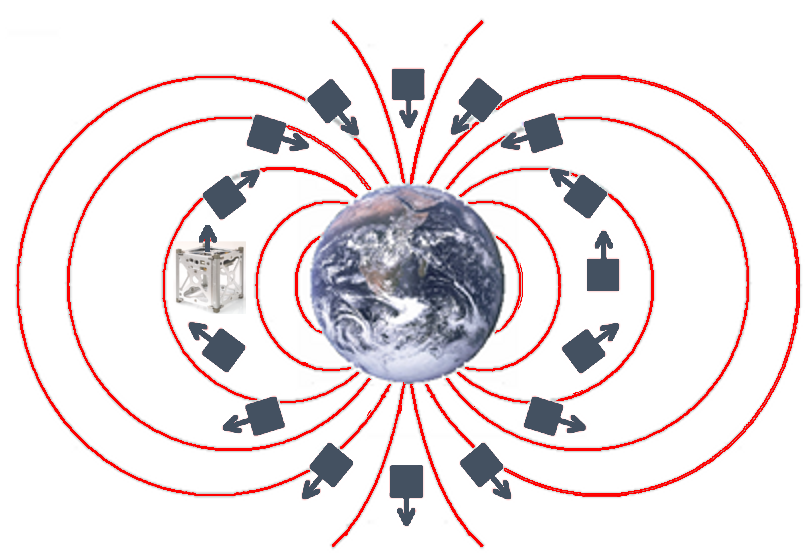
\includegraphics[width=0.6\linewidth]{./figs/Mag_Field}
	
	\begin{small}
		FONTE: \cite{FrancLav}
	\end{small}
	\label{fig:Mag_Field}
\end{figure}

\newpage

O método da estabilização por rotação é uma melhoria do método passivo por alinhamento. Nele, o satélite permanece apontado para uma posição fixa e rotaciona ao redor do eixo principal. Apesar do controle não permitir mudanças bruscas no apontamento do eixo principal, que assim como o método passivo, deve ser definido durante a fase de projeto, essa rotação cria uma inércia que o torna robusto a perturbações, aumentando a precisão do apontamento \cite{FrancLav}.

O método da propulsão é muito pouco utilizado em CubeSats. Consiste em jatos de gás ou foguetes monopropulsores, que trabalham normalmente em pares, posicionados ao redor do satélite de forma que gerem um impulso inicial, provocando um torque. A vantagem dessa forma de controle é que pode ser usada também para translação do CubeSat, como ilustrado na Figura \ref{fig:Propulsion} a seguir. Porém, como ocupa muito espaço, tanto para o próprio propulsor quanto para o combustível que utiliza, é utilizado apenas em CubeSats com pelo menos 3U \cite{Luka}.

\begin{figure}[th]
	\caption{Controle através de propulsão.}
	\centering
	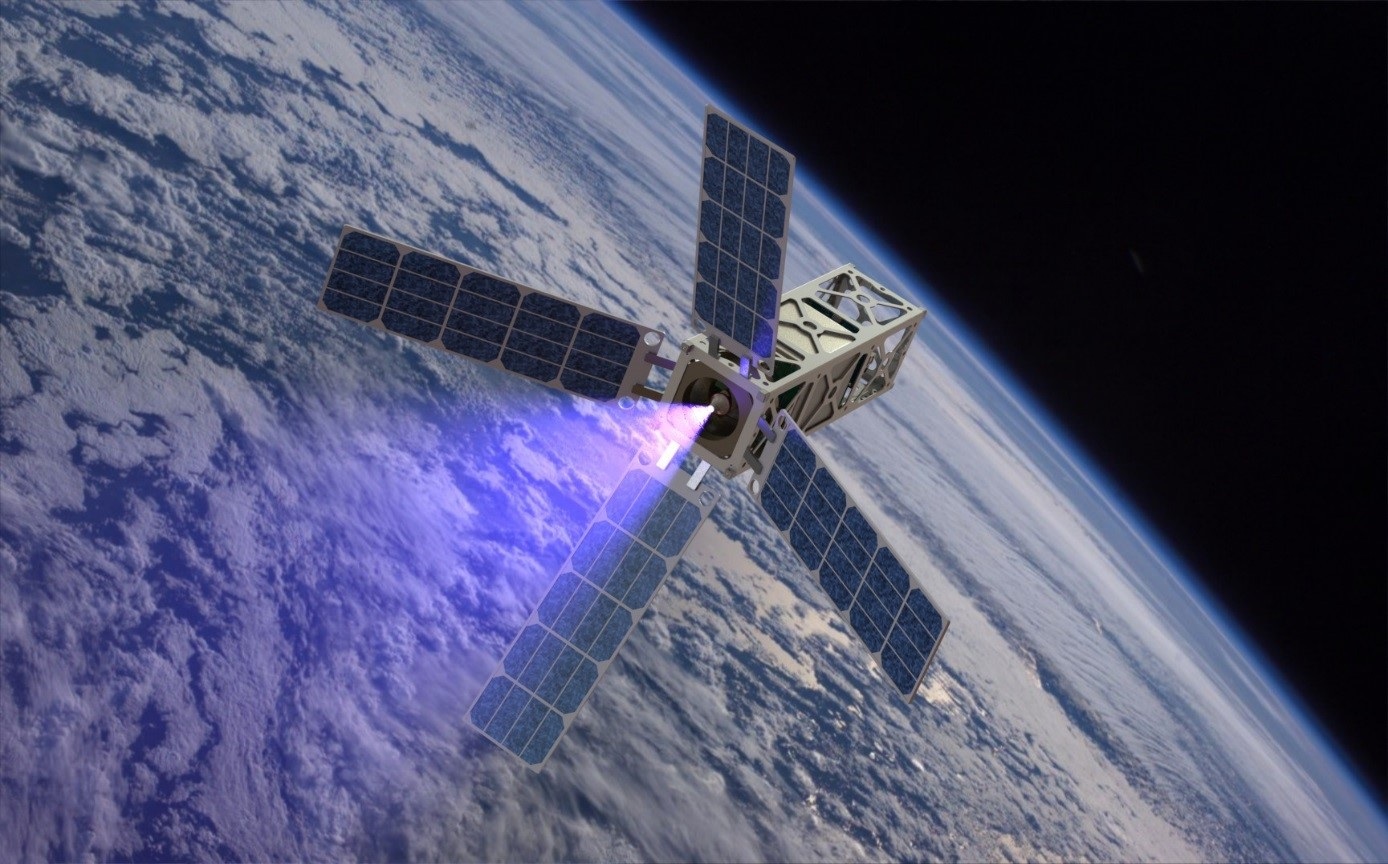
\includegraphics[width=0.6\linewidth]{./figs/Propulsion}
	
	\begin{small}
		FONTE: \cite{Prop}
	\end{small}
	\label{fig:Propulsion}
\end{figure}

%\newpage

O método da estabilização dos três eixos é o método mais comumente utilizado, já que é versátil e usa pouco espaço, além de ser o mais eficiente. Ele se baseia na terceira Lei de Newton, que diz: \textit{''Para toda ação, há sempre uma reação oposta e de igual intensidade''}. Isso significa que se há uma massa acelerando presa ao satélite, ela irá forçar o mesmo a girar na direção oposta. Quanto maior o valor dessa massa, mais influência ela terá sobre o sistema \cite{Ericksson}. As rodas de reação fazem o papel dessa massa ao serem fixadas ao eixo de motores (normalmente \textit{brushless}) e dispostos cada um em um eixo, possibilitando realizar manobras de rolagem (\textit{roll} ou X), arfagem (\textit{pitch} ou Y) e guinada (\textit{yaw} ou Z). Um exemplo desse conjunto de motor e roda de reação é mostrado a seguir, na Figura \ref{fig:SRW}.

\begin{figure}[th]
	\caption{Conjunto motor e roda de reação.}
	\centering
	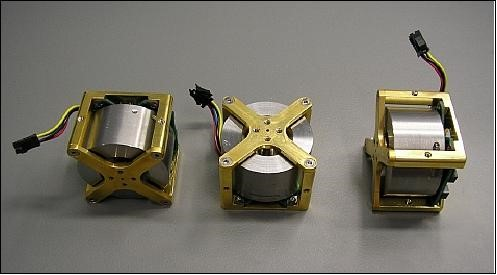
\includegraphics[width=0.7\linewidth]{./figs/Shelf_Reaction_Wheel}
	
	\begin{small}
		FONTE: \cite{SWR}
	\end{small}
	\label{fig:SRW}
\end{figure}

%\newpage 

Há ainda dois tipos de controle através desse método, um com quatro e outro com três conjuntos motor-roda de reação. O modelo que utiliza quatro conjuntos possui controle mais complexo, uma vez que estes conjuntos são dispostos de forma que o somatório das rotações forma o torque desejado, como mostra a Figura \ref{fig:ERW} a seguir. Este método é amplamente utilizado pois caso um dos motores pare de funcionar, os outros três podem compensa-lo, aumentando a vida útil do satélite \cite{Ericksson}.

\begin{figure}[th]
	\caption{Modelo com quatro conjuntos motor-roda de reação e duas hastes magnéticas.}
	\centering
	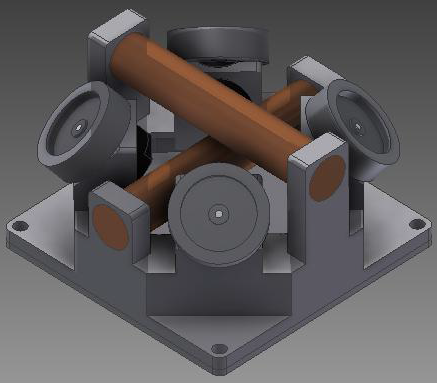
\includegraphics[width=0.6\linewidth]{./figs/Ericksson_Reaction_Wheel}
	
	\begin{small}
		FONTE: \cite{Ericksson}
	\end{small}
	\label{fig:ERW}
\end{figure}

\newpage

Já o modelo de três conjuntos motor-roda de reação é mais simples, cada conjunto atua diretamente em um eixo, controlando-o diretamente, como mostrado a seguir pela Figura \ref{fig:3RW}. Sua maior desvantagem é que caso um dos motores pare de funcionar, o movimento do satélite no eixo correspondente também cessa. Esse é o método adotado e explorado nesse trabalho.

\begin{figure}[th]
	\caption{Modelo com três conjuntos motor-roda de reação.}
	\centering
	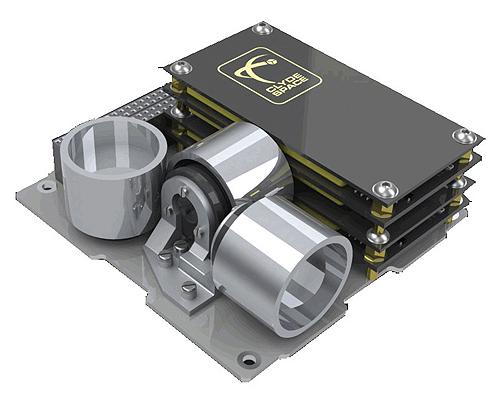
\includegraphics[width=0.7\linewidth]{./figs/3RW}
	
	\begin{small}
		FONTE: \cite{3RW}
	\end{small}
	\label{fig:3RW}
\end{figure}

%\newpage

% ----------------------------------------------------------
% Materiais e Métodos
% ----------------------------------------------------------
%\chapter[Materiais e Métodos]{Materiais e métodos}

%Para facilitar a compreensão das partes que envolvem o projeto, os itens foram divididos em duas categorias:
%Materiais, focada em explicar quais os materiais utilizados para a construção do CubeSat e porquê.
%Métodos, focada em explicar como foi feita a integração dos materiais, programações necessárias, cálculos de equações de modelagem e controle, etc.

% ----------------------------------------------------------
% Materiais
% ----------------------------------------------------------
\chapter{Materiais}

Os materiais utilizados para a construção de CubeSats são COTS, isso significa que a maior parte deles foi comprada e implementada diretamente, sem necessidade de adaptações.

\section{Sensor}

Como a determinação de atitude não é objeto de estudo deste trabalho, não será abordado um método para escolha do melhor sensor. Adotamos uma \textit{Inertial Measurement Unit} (IMU) HMC6343 (Honeywell, EUA), mostrado a seguir na Figura \ref{fig:IMU}, que é a combinação de três magnetômetros e três acelerômetros, cada um disposto em um eixo, de forma a compor as informações de rotação dos três eixos. Sua precisão é de cerca de $1^{\circ}$ em para \textit{Roll} e \textit{Pitch} e $2^{\circ}$ para \textit{Yaw}, uma precisão ótima para a nossa aplicação, além de ter um tamanho extremamente compacto (9x9mm). Essa IMU fornece os dados já tratados através de uma porta de comunicação I$^{2}$C.

\begin{figure}[th]
	\caption{IMU utilizada.}
	\centering
	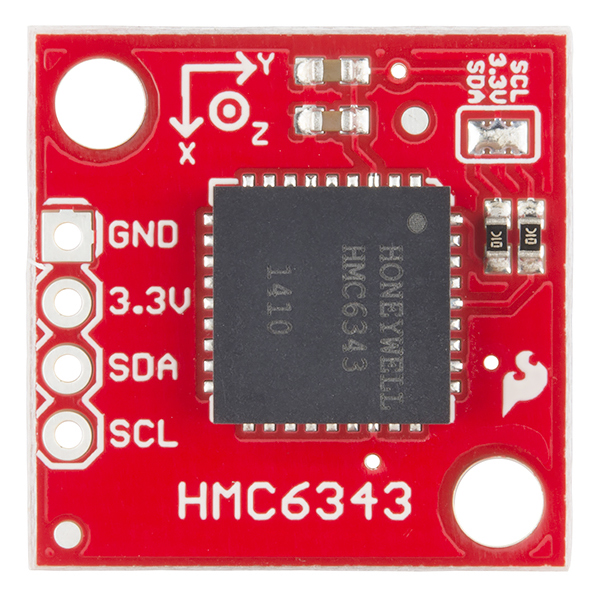
\includegraphics[width=0.425\linewidth]{./figs/IMU-HMC6343}
	
	\begin{small}
		FONTE: \cite{IMU}
	\end{small}
	\label{fig:IMU}
\end{figure}

%\newpage

\section{Circuitos e componentes eletrônicos}

O objetivo do conjunto de circuitos eletrônicos é possibilitar o controle de velocidade independente dos três motores, cada um com um microcontrolador, um driver e um sensor de corrente. Para comandar o conjunto é necessário um microcontrolador principal, responsável por enviar \textit{set points} de velocidades de acordo com a leitura do sensor de posicionamento conforme definido pela sua malha de controle. A comunicação entre esses quatro dispositivos é realizada por duas redes I$^{2}$C: uma para leitura do sensor e uma para comunicação entre microcontroladores.

As soluções de hardware que satisfazem os requisitos de desempenho para um Cubesat são abundantes no mercado internacional \cite{STATEOFART}. Desta forma os critérios de escolha muitas vezes são o custo, o risco e a disponibilidade dos itens no fabricante.

\subsection{Microcontrolador}

A capacidade de processamento que um satélite precisa já está disponível no mercado. A velocidade recomendada de um processador para um CubeSat é de aproximadamente 30 MIPS. Além do tamanho dos componentes, sempre é necessário um cuidado especial com o consumo de energia \cite{STATEOFART}.

Os microprocessadores selecionados foram da família dsPIC33EP. Eles possuem capacidade de processamento de 60 MIPS operando de $-40^{\circ}$C até $+125^{\circ}$C. Possuem modo de gerenciamento de baixo consumo de energia, módulo DSP, que consiste em um multiplicador de alta velocidade capaz de realizar multiplicações com 17 bits e somas ou subtrações com 40 bits. Seu diferencial para controle de motores BLDC aparece em seus três módulos independentes de PWM de alta velocidade, que podem gerar disparos ao modulo ADC. Outra ferramenta que será utilizada no controle do motor é o \textit{Input Capture}, que é utilizado em aplicações que requerem medidas de períodos e frequências \cite{dsPIC33EP}. Todas essas ferramentas serão compiladas no ambiente MPLAB X IDE utilizando o compilador XC16, ambos do fabricante Microchip.

O microcontrolador utilizado na placa de controle é o dsPIC33EP32MC502 (Microchip, EUA) onde o seu circuito é apresentado na Figura \ref{fig:dsPIC502} a seguir. 

\begin{figure}[th]
	\caption{Microcontrolador dsPIC33EP32MC502.}
	\centering
	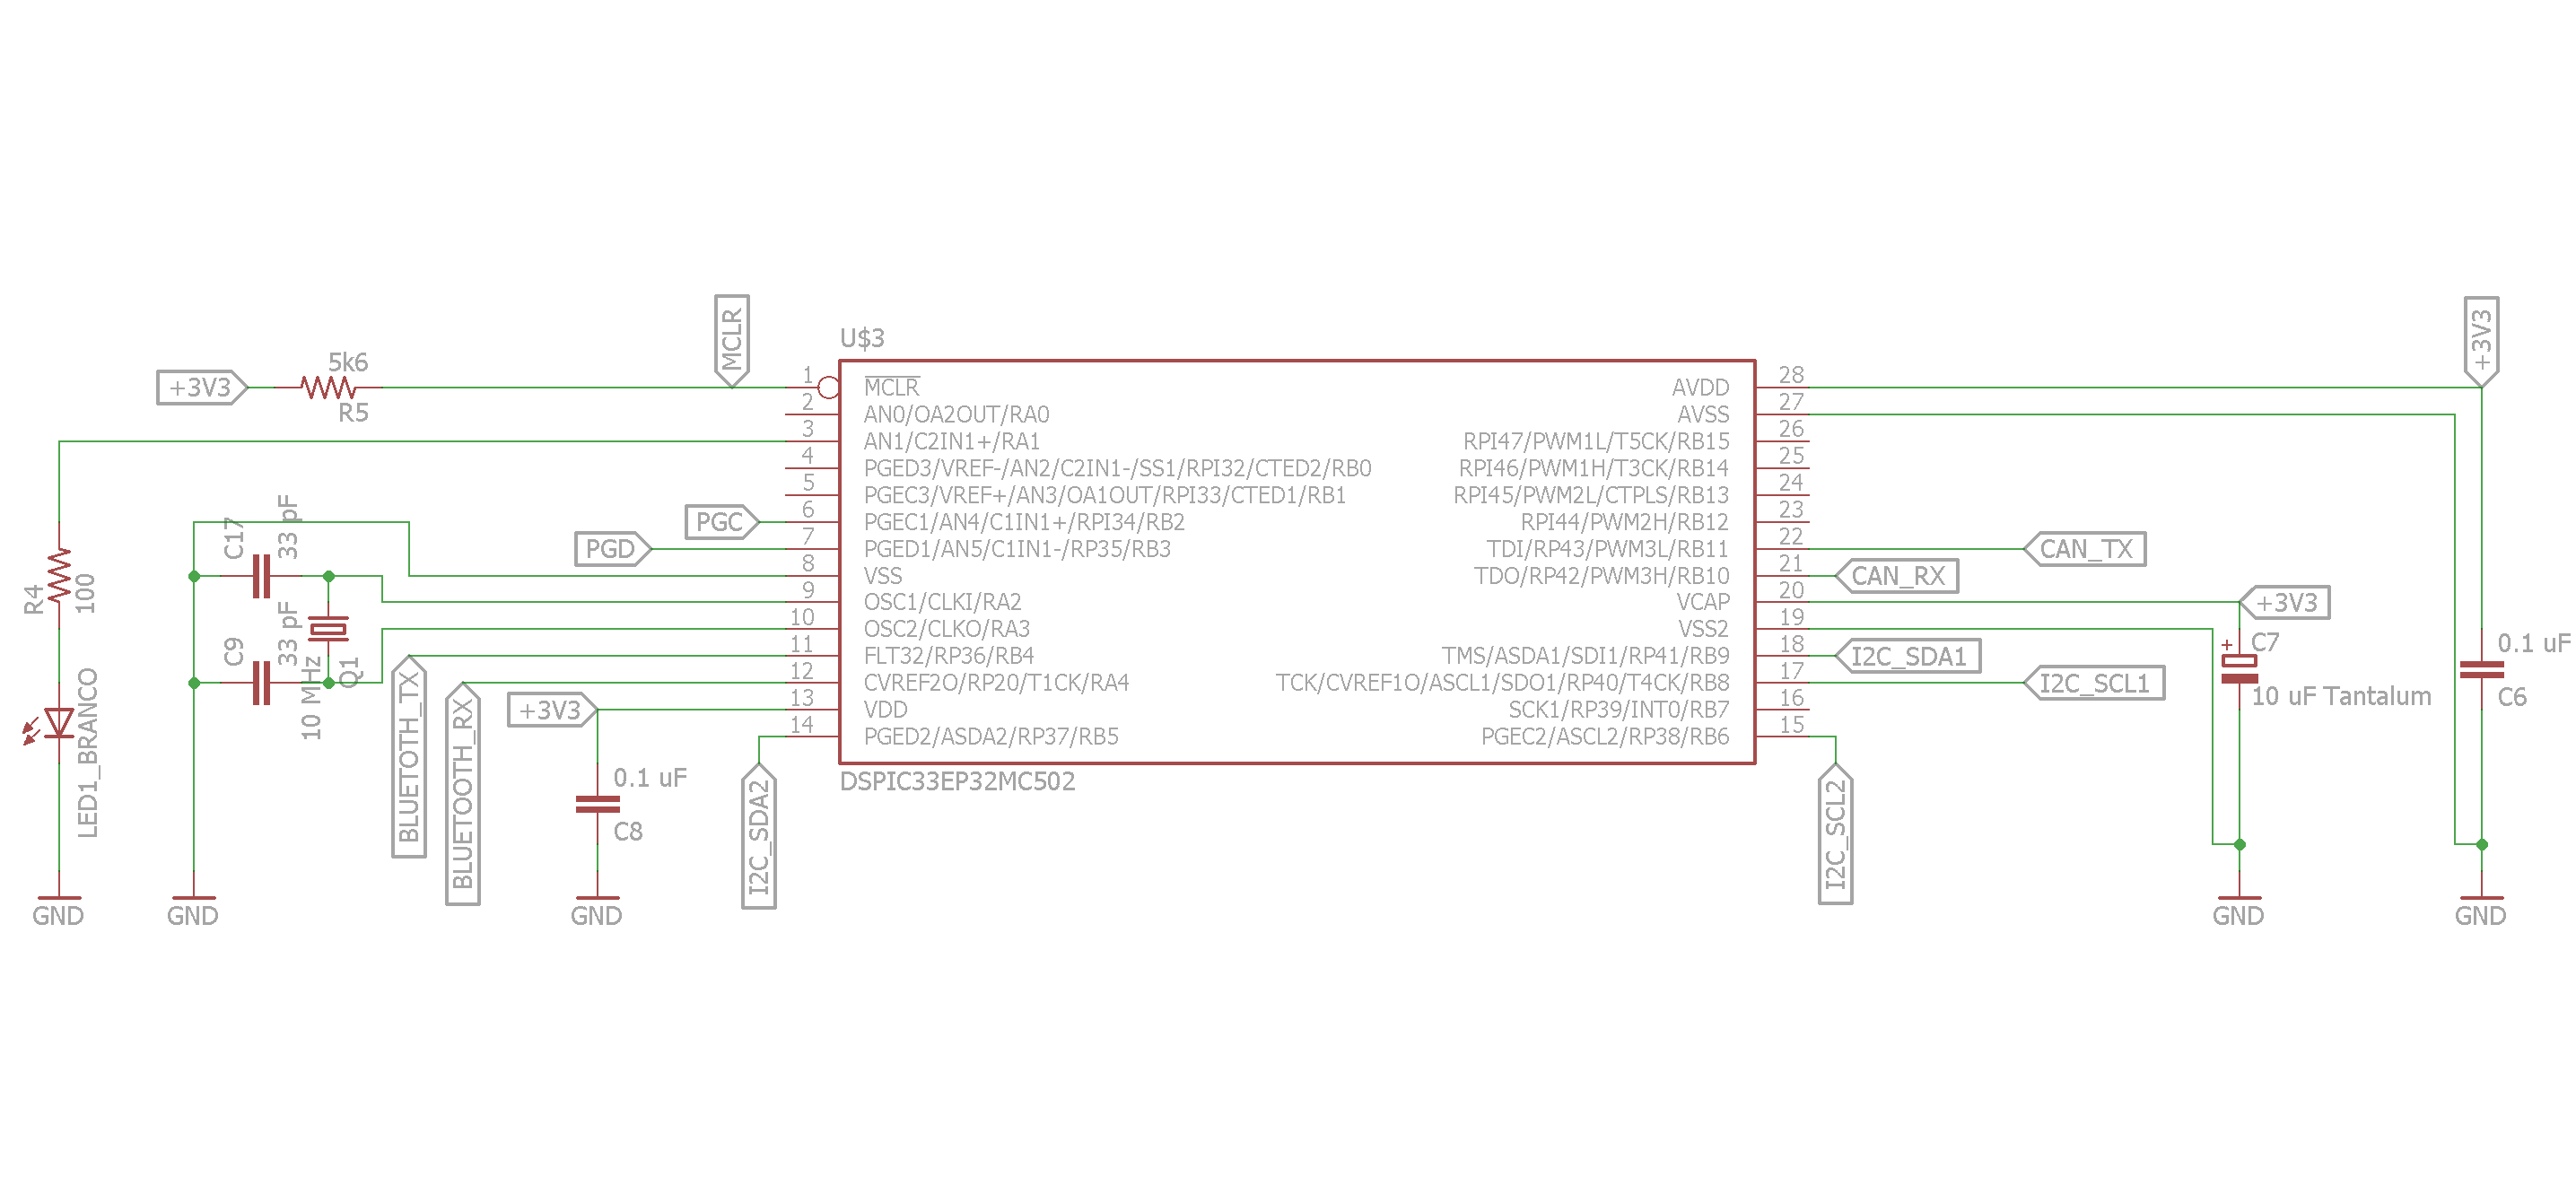
\includegraphics[height=1.2\linewidth]{./figs/dsPIC_master}
	
	\begin{small}
		FONTE: Arquivo dos autores.
	\end{small}
	\label{fig:dsPIC502}
\end{figure} 

\newpage

O microcontrolador utilizado na placa de acionamento do motor é o dsPIC33EP32MC202 (Microchip, EUA) onde o seu circuito é apresentado na Figura \ref{fig:dsPIC202} a seguir.

\begin{figure}[th]
	\caption{Microcontrolador dsPIC33EP32MC202.}
	\centering
	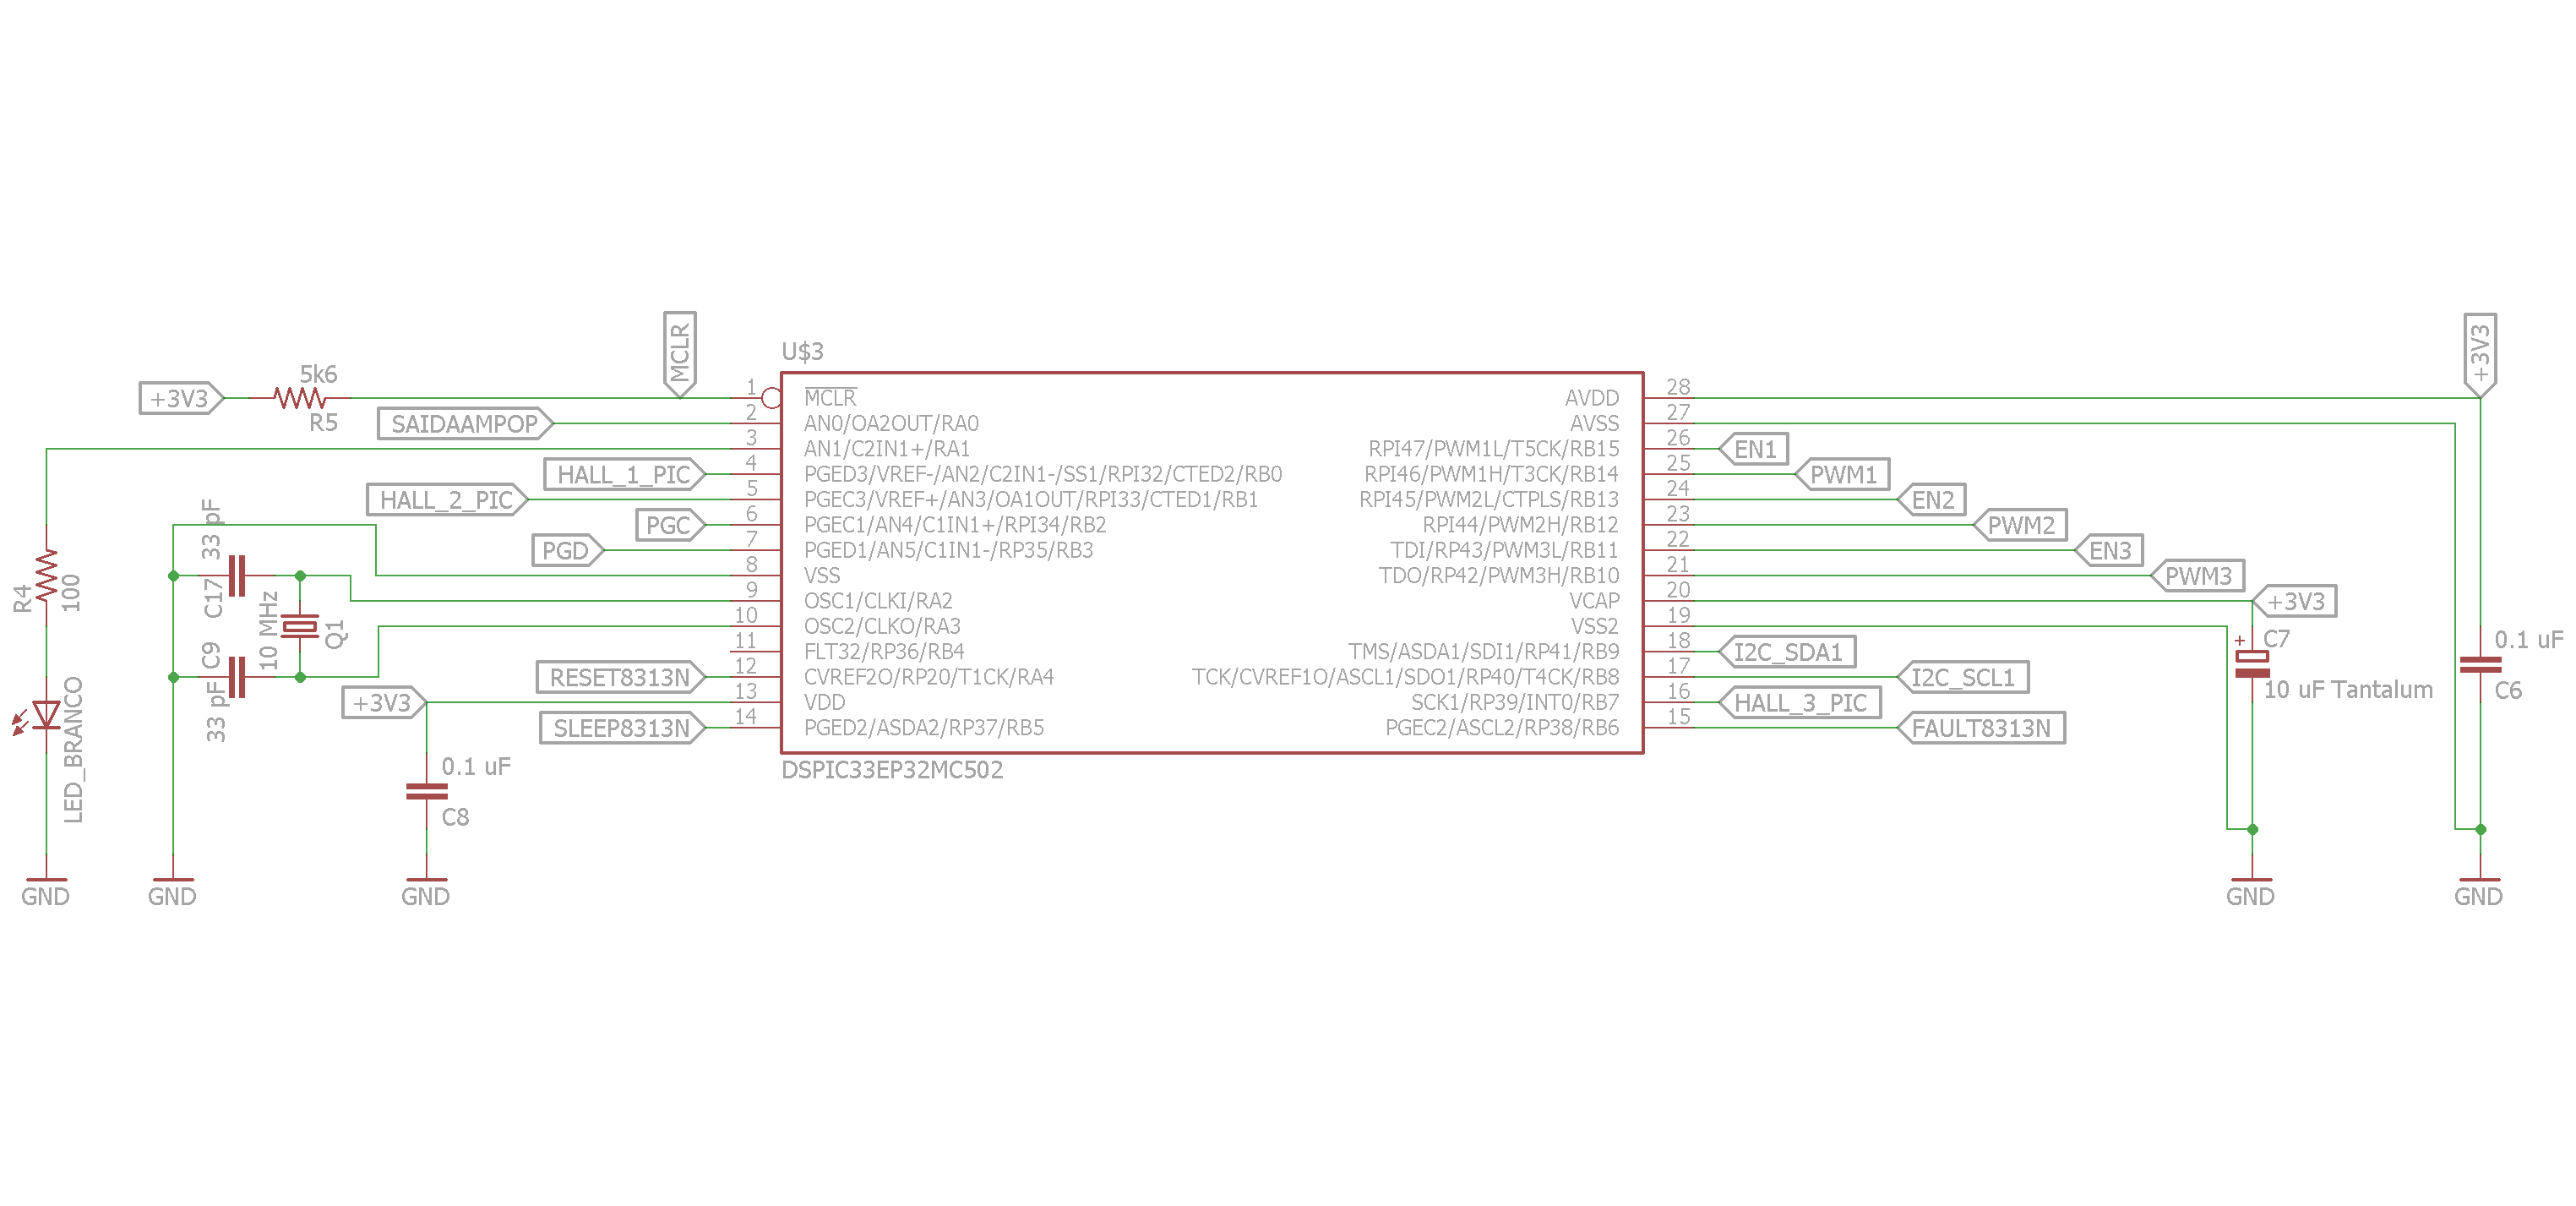
\includegraphics[height=1.2\linewidth]{./figs/dsPIC_motores}
	
	\begin{small}
		FONTE: Arquivo dos autores.
	\end{small}
	\label{fig:dsPIC202}
\end{figure} 

\newpage

\subsection{\textit{Driver} de acionamento do motor}

Para o acionamento do motor foi selecionado o circuito integrado DRV8313 (Texas Instruments, EUA). O DRV8313 possui três meias pontes H que suportam $2.5A$ de corrente de pico e podem alimentar o motor com tensões de $8$ a $60V$ além de possuir circuitos de proteção contra sobre-corrente, curto circuito e subtenção.\cite{DRV8313}. O driver destina-se a aplicações de acionamento de motores BLDC de três fases, mas pode ser utilizado também para acionamento de solenoides. Possui a funcionalidade de \textit{sleep mode}, que pode ser ativada quando não é preciso fazer controle de velocidade do motor e auxilia no consumo de energia e por fim pode reportar falhas em sua operação através do pino \textit{FAULT}, conforme a Figura \ref{fig:Driver} a seguir.

\begin{figure}[th]
	\caption{Driver DRV8313.}
	\centering
	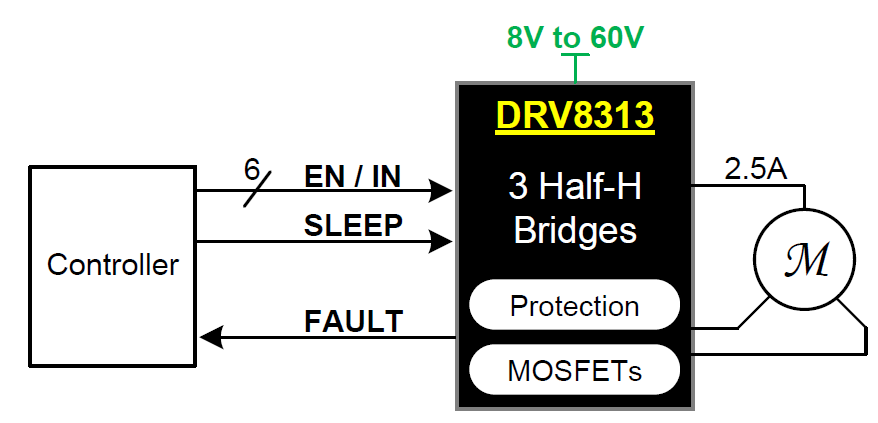
\includegraphics[width=0.6\linewidth]{./figs/DRV8313-fig}
	
	\begin{small}
		FONTE: \cite{DRV8313}
	\end{small}
	\label{fig:Driver}
\end{figure}

%\newpage

\subsection{Interfaces e barramentos}

Enquanto os famosos \textit{Universal Serial Bus} (USB) e o \textit{Controller Area Network} (CAN) são protocolos de comunicação usados esporadicamente, o protocolo I$^{2}$C aparece como o barramento mais utilizado para nano satélites, devido ao seu baixo consumo de energia, além de estar disponível na maioria dos microcontroladores. Outros tipos de interfaces para diferentes tipos de fluxo de dados são desejáveis. \cite{STATEOFART}

O barramento de comunicação da placa de controle é composto por duas redes I$^{2}$C, uma para a comunicação com a IMU e outra para a comunicação com os outros microcontroladores. Também estão disponíveis no conjunto uma interface CAN e uma USART – \textit{Universal Synchronous/Asynchronous Receiver/Transmitter} além de interface ICSP – \textit{In-Circuit Serial Programming} para a programação do microcontrolador.

%\begin{figure}[th]
%	\caption{Barramento de comunicação.}
%	\centering
%	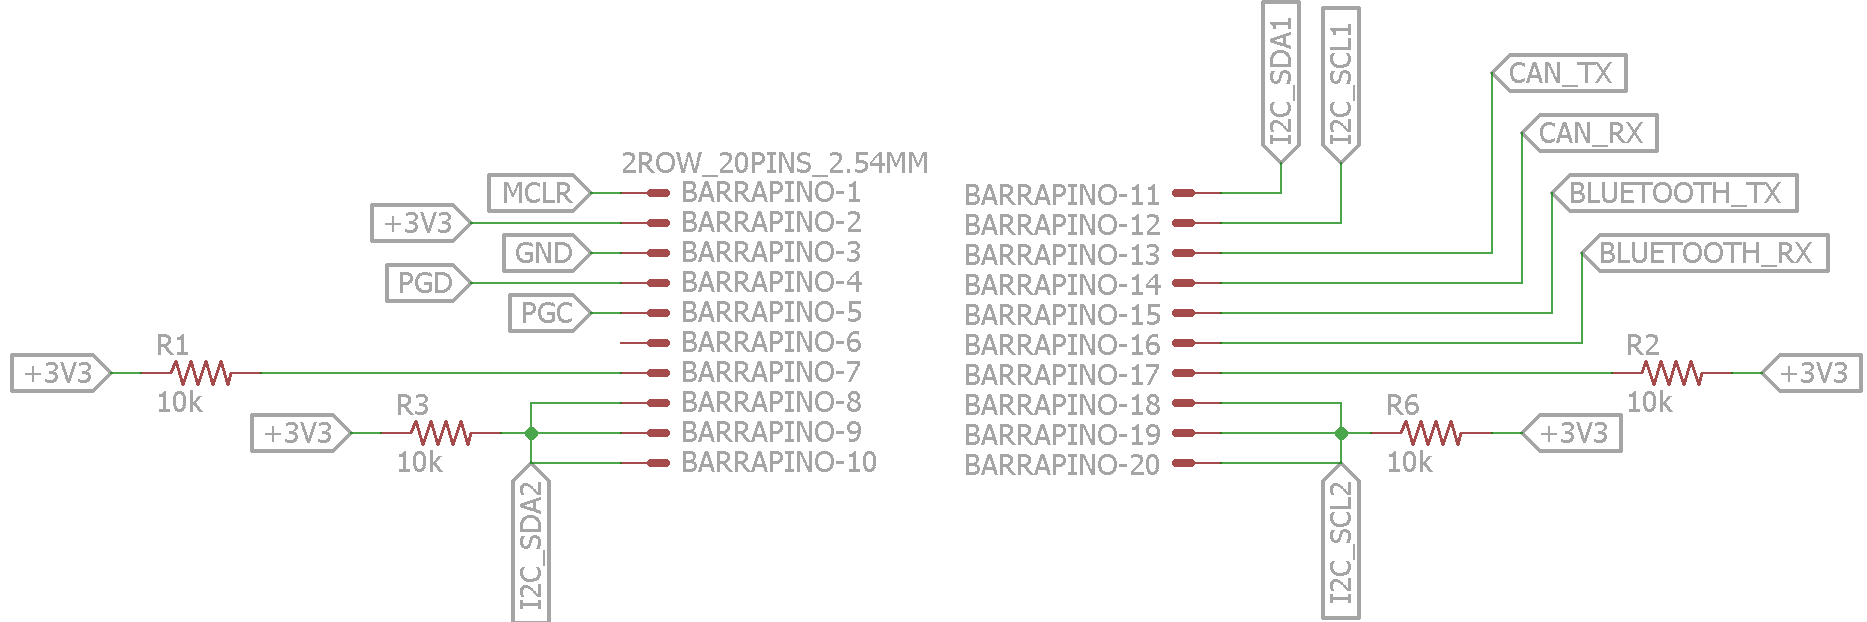
\includegraphics[width=0.8\linewidth]{./figs/Barra_pino_master}
	
%	\begin{small}
%		FONTE: Arquivo dos autores.
%	\end{small}
%	\label{fig:Barra_pino_master}
%\end{figure}

A placa de controle é responsável também por receber a alimentação 12V da bateria e distribuir para as outras placas através de seu barramento de alimentação.

%\begin{figure}[th]
%	\caption{Barramento de alimentação.}
%	\centering
%	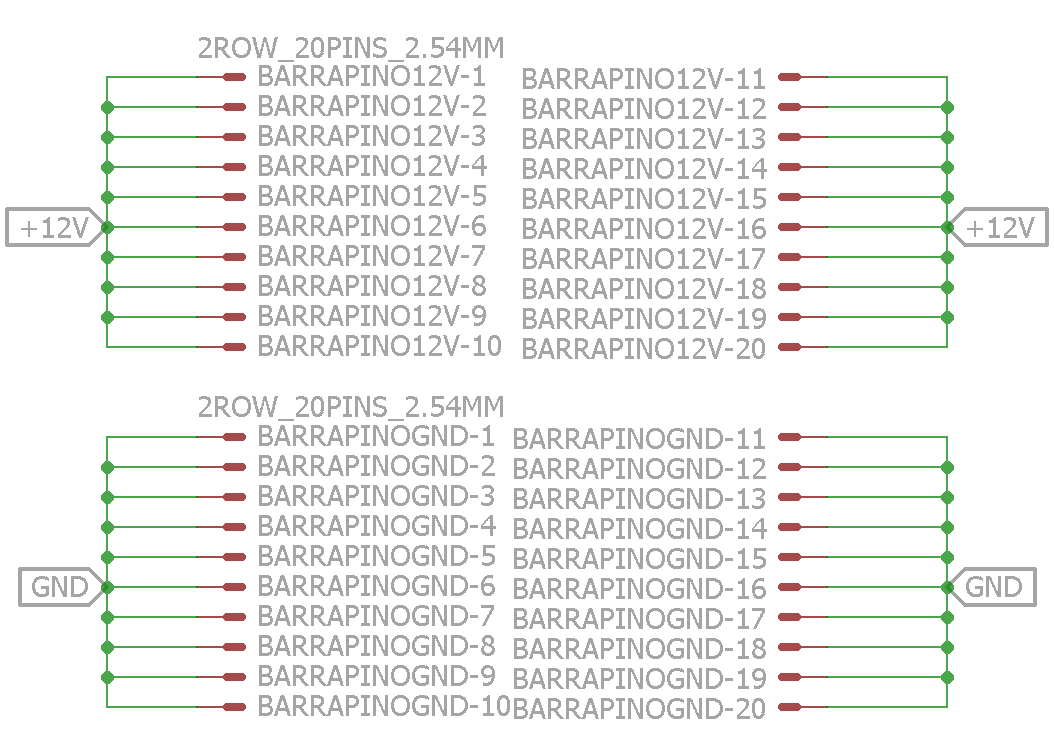
\includegraphics[width=0.8\linewidth]{./figs/Barra_pino_alimentacao_master}
	
%	\begin{small}
%		FONTE: Arquivo dos autores.
%	\end{small}
%	\label{fig:Barra_pino_alimentacao_master}
%\end{figure} 

No barramento de comunicação da placa de acionamento do motor, existe interface para comunicação I$^{2}$C, alimentação e interface ICSP – \textit{In-Circuit Serial Programming} para programação do microcontrolador.

%\begin{figure}[th]
%	\caption{Barramento da placa de motor.}
%	\centering
%	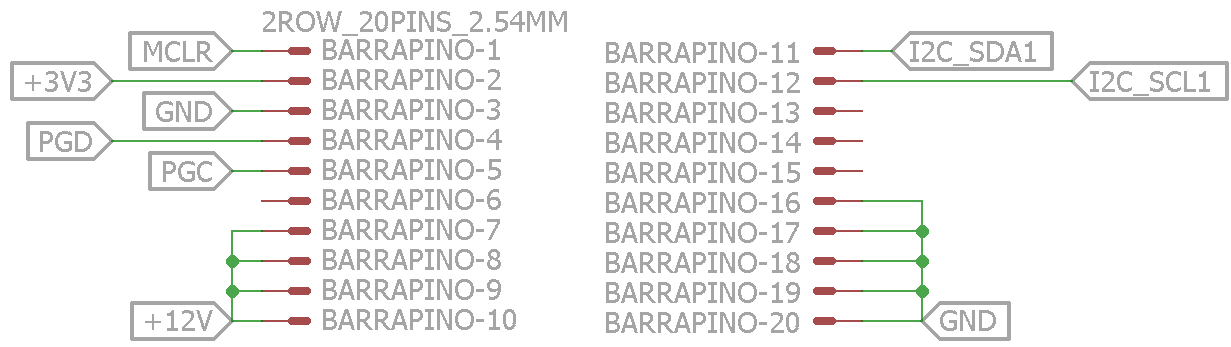
\includegraphics[width=0.8\linewidth]{./figs/Barra_pino_motores}
	
%	\begin{small}
%		FONTE: Arquivo dos autores.
%	\end{small}
%	\label{fig:Barra_pino_motores}
%\end{figure} 

\subsection{Medidor de corrente}

Para o sistema de controle do BLDC é necessário conhecer a corrente que está passando pelo motor. A aquisição é feita através da medição de tensão sobre um resistor \textit{shunt} de $0,5\Omega$ colocado  em série com o motor. 

O valor dessa tensão é muito pequeno, variando de 0 até 243mV quando o motor estiver com 100\% de PWM, sendo assim necessária a amplificação desse sinal. Para isso foi utilizado um amplificador operacional LMV358 (Texas Instruments, EUA) configurado conforme a Figura \ref{fig:Medidor_corrente}.

\begin{figure}[th]
	\caption{Medidor de corrente.}
	\centering
	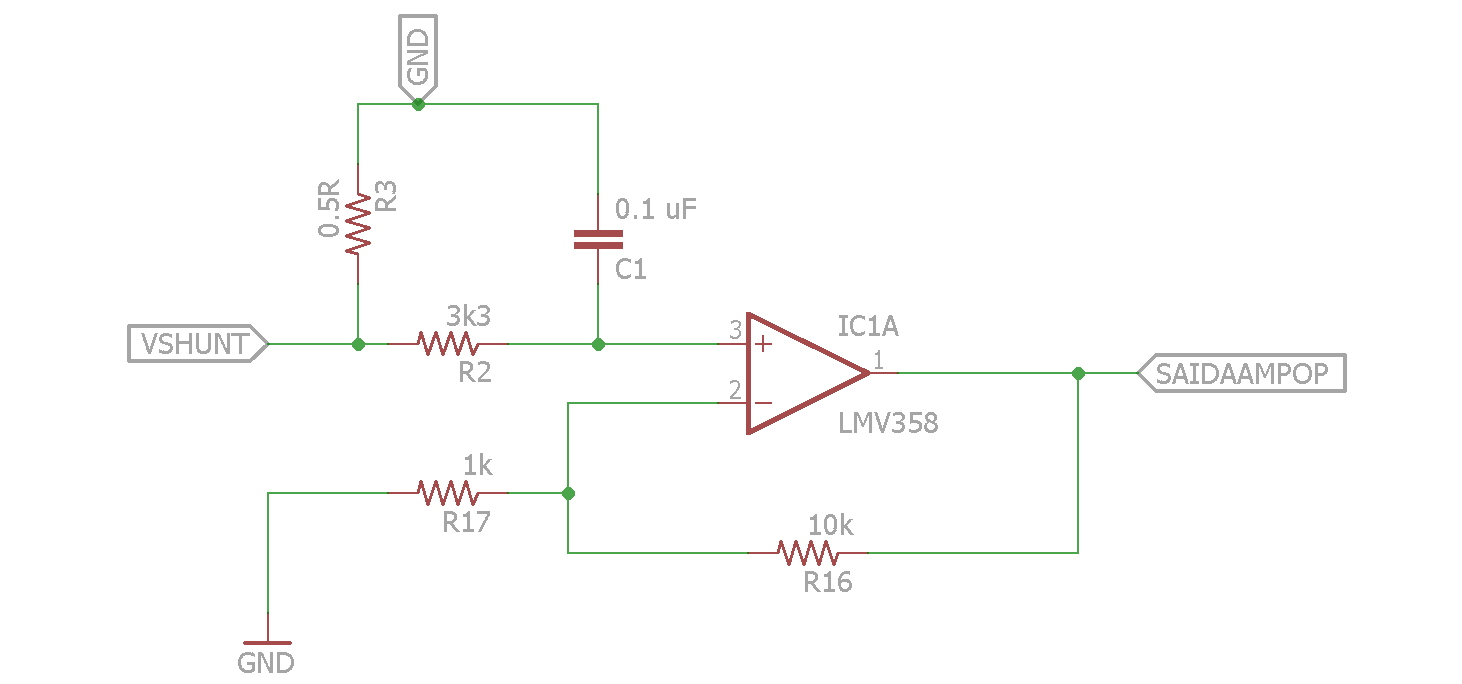
\includegraphics[width=1\linewidth]{./figs/Medidor_corrente_motores}
	
	\begin{small}
		FONTE: Arquivo dos autores.
	\end{small}
	\label{fig:Medidor_corrente}
\end{figure}

%\newpage

Como pode ser observado na imagem, existe um filtro com frequência de corte de 482Hz com o objetivo de filtrar pequenos ruídos e a forma de onda do PWM, pois estes também serão amplificados se não filtrados, prejudicando a medição da tensão.

O amplificador está configurado para que sua saída que é não inversora ter uma ganho de 11 vezes em relação a sua entrada, ou seja, a sua saída terá o valor máximo de aproximadamente 2,7V.

A saída do amplificador operacional é conectada em uma entrada do microcontrolador que possua o módulo de conversão analógica para que seja feita a conversão do sinal para valor digital.  

\subsection{Divisor de tensão com resistências}

Os sensores de efeito Hall do motor possuem alimentação de 12V porém o microcontrolador é tolerante com tensões de até 5V. Nesse caso é necessário a construção de um divisor de tensão com resistências  conforme a Figura \ref{fig:Divisor_tensao}. 

\begin{figure}[th]
	\caption{Divisor de tensão com resistências.}
	\centering
	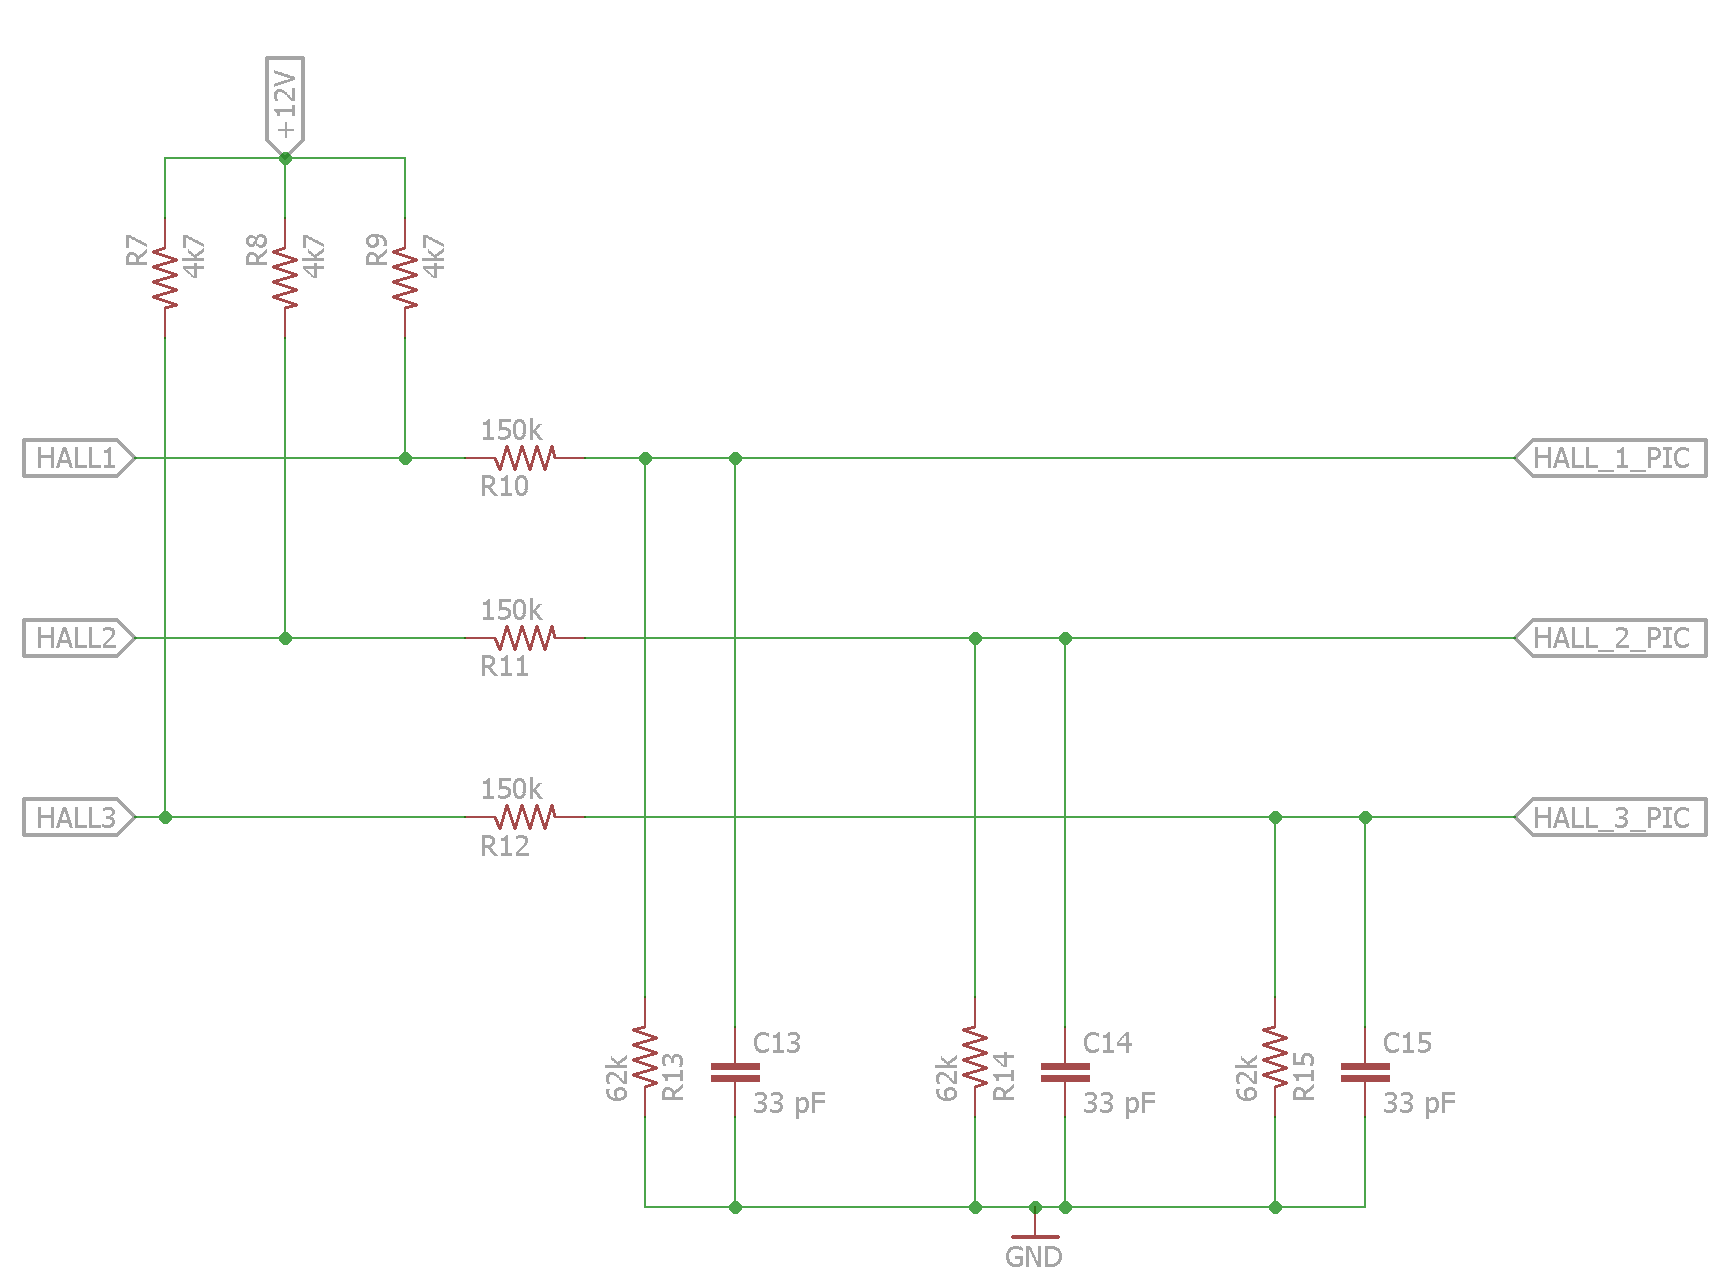
\includegraphics[width=0.75\linewidth]{./figs/Halls_motores}
	
	\begin{small}
		FONTE: Arquivo dos autores.
	\end{small}
	\label{fig:Divisor_tensao}
\end{figure}

\newpage

Os resistores foram dimensionados de forma que a tensão de saída seja igual a 3,51V. Foi elaborado também um filtro com frequência de corte de 32153Hz para filtrar pequenos ruídos e também \textit{pull-up} em cada sensor Hall do motor.

\subsection{Regulador de tensão}

As placas eletrônicas são alimentadas com 12V porém, toda a parte lógica do circuito deve ser alimentada 3,3V. Nesta situação, é utilizado o regulador de tensão REG1117-3.3 (Texas Instruments, EUA) que retifica a tensão de 12V para 3,3V e possui a capacidade de fornecer até 800mA, o suficiente para alimentar todos os componentes.

\subsection{Placas de circuito eletrônico}

Devido ao espaço reduzido dentro do CubeSat, é necessário dividir funções para cada placa eletrônica, ou seja, o CubeSat possui uma placa de controle e três placas responsáveis cada uma por acionar um motor.

\subsubsection{Placa de controle}

A placa de controle é responsável por receber os dados da IMU, processar esse dados, gerar o \textit{set point} de cada motor e enviar esse \textit{set point} para sua respectiva placa de acionamento. Essa placa possui os seguintes componentes e circuitos: microcontrolador, regulador de tensão, barramento de comunicação e barramento de alimentação. A placa de circuito eletrônico pode ser vista no Apêndice \ref{ap:PMaster}. 

\subsubsection{Placa de acionamento dos motores}

A placa de acionamento dos motores é responsável por receber o \textit{set point} da placa de controle, fazer o controle da ordem de acionamento das bobinas do motor através dos sensores de efeito Hall, medir a corrente que está passando pelo motor, processar a lei de controle e acionar o motor. A placa de acionamento possui um regulador de tensão, um divisor de tensão, um circuito medidor de corrente, barramento de comunicação e barramento de alimentação.  A placa de circuito eletrônico pode ser vista no Apêndice \ref{ap:PMotor}.

\subsubsection{Lista de componentes}

A seguir, na Tabela \ref{tab:CompElet}, a lista de componentes usados na confecção de ambas as placas. Nos locais onde há um asterisco indicado, o componente é compartilhado entre ambas as placas.

\begin{table}[h]
	\caption{Lista de componentes eletrônicos.}
		\centering
	\begin{tabular}{|c|c|c|}
		\hline
		\textbf{Descrição} & \textbf{Quantidade} & \textbf{Quantidade}\\
		  & \textbf{placa motor} & \textbf{placa controle} \\
		\hline 
		Regulador de tensão REG1117 & 1 & 1 \\ 
		\hline 
		Conector  1-84953-1 & 1 & \\ 
		\hline 
		Resistor shunt $0,5\Omega$, 1W, 1\% & 1 & \\
		\hline 
		Amplificador operacional LMV358 & 1 & \\
		\hline 
		Circuito integrado DRV8313 & 1 & \\
		\hline 
		Microcontrolador dsPIC33EP32MC502 & 1 & 1 \\
		\hline 
		Capacitor eletrolítico $47\mu$F & 4 & 4 \\
		\hline
		Capacitor eletrolítico $10\mu$F & 1 & \\
		\hline
		Capacitor cerêmico $0,1\mu$F & 7 & 2 \\
		\hline
		Capacitor cerêmico 33pF & 5 & 2 \\
		\hline
		Capacitor de tântalo $10\mu$F & 1 & 1 \\
		\hline
		Resistor $100\Omega$ & 2 & 1 \\
		\hline
		Resistor $1k\Omega$ & 1 & \\
		\hline
		Resistor $3k3\Omega$ & 1 & \\
		\hline
		Resistor $4k7\Omega$ & 3 & \\
		\hline
		Resistor $5k6\Omega$ & 1 & 1 \\
		\hline
		Resistor $10k\Omega$ & 1 & 4 \\
		\hline
		Resistor $62k\Omega$ & 3 & \\
		\hline
		Resistor $150k\Omega$ & 3 & \\
		\hline
		Led branco & 1 & 1 \\
		\hline
		Led verde & 1 & \\
		\hline
		Cristal 10MHz & 1 & 1 \\
		\hline
		Barra de pino 20x2 & 1 & 3 \\
		\hline
		Bateria 1300mAh & 1 & * \\
		\hline
		Conector XT60 fêmea & 1 & * \\
		\hline
		Módulo bluetooth HM-10 & 1 & * \\
		\hline
		Cabinho jumper & 60 & * \\
		\hline
	\end{tabular}
	
	\begin{small}
	\vspace{3pt}	
	FONTE: Dos autores.
	\end{small}
	\label{tab:CompElet}
\end{table}

\newpage

\section{Atuador}

Para integração do motor adotado com a roda de ação, foi criado um conjunto padrão que consiste em um suporte para o motor, o motor e a roda de reação. Foi utilizado um desses conjuntos em cada um dos eixos correspondentes ao \textit{roll}, \textit{pitch} e \textit{yaw} como mostrado na Figura \ref{fig:MotSet} a seguir.

\begin{figure}[th]
	\caption{Conjunto para acoplamento do motor ao CubeSat.}
	\centering
	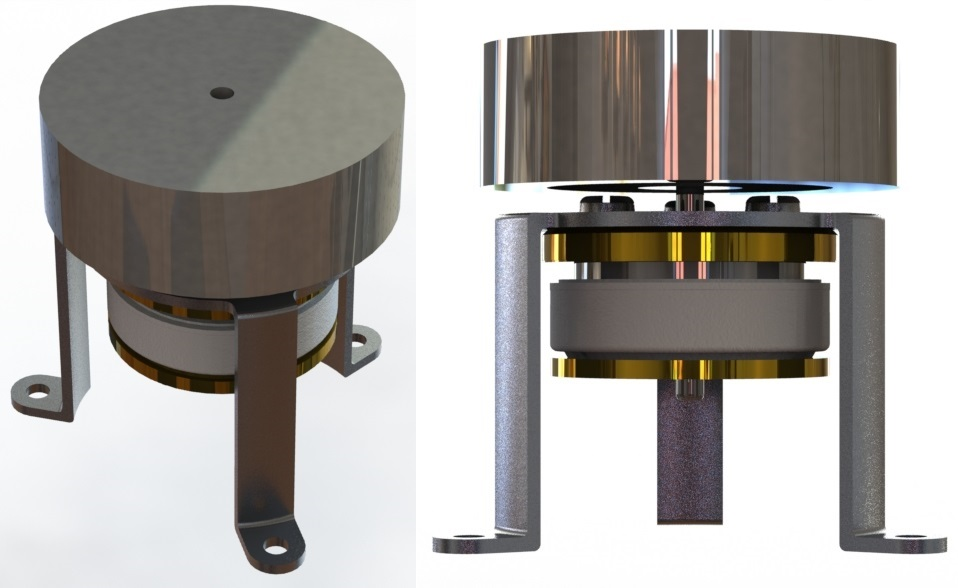
\includegraphics[width=0.7\linewidth]{./figs/Motor_Set}
	
	\begin{small}
		FONTE: Arquivo dos autores.
	\end{small}
	\label{fig:MotSet}
\end{figure}

\newpage

\subsection{Motor}

Para escolha do motor, foi levado em consideração principalmente dois fatores: tipo e tamanho \cite{Ericksson}.

Costumeiramente, CubeSats utilizam motores de corrente contínua sem escovas (\textit{brushless direct current motor} – BLDC). A NASA recomenda o uso de motores desse tipo para aplicações aeroespaciais \cite{NASABLDC}. A Tabela \ref{tab:VnteDesv} a seguir mostra um comparativo das principais vantagens do uso de um motor \textit{brushless} na área aeroespacial segundo a NASA.

\begin{table}[h]
	\caption{Vantagens e desvantagens de um motor \textit{Brushless}.}
		\centering
	\begin{tabular}{|c|c|}
		\hline
		\textbf{Vantagens} & \textbf{Desvantagens} \\ 
		\hline 
		Alta velocidade (até 100000RPM) & Circuitos mais caros \\ 
		\hline 
		Alto torque a altas velocidades & Maior complexidade do driver do motor \\ 
		\hline 
		Aproximadamente o dobro de torque & \\
		 de saída quando comparado a motores & \\
		  com escova do mesmo tamanho &  \\ 
		\hline 
		Enrolamentos no estator ao invés & \\
		 do rotor melhoram a dissipação & \\
		  de calor & \\ 
		\hline 
		Sem escovas, então os motores & \\
		 duram enquanto durarem os & \\
		  rolamentos & \\ 
		\hline 
		Alta eficiência & \\ 
		\hline 
		Bom desempenho no vácuo & \\ 
		\hline
	\end{tabular}
	
	\begin{small}
	\vspace{3pt}	
	FONTE: \cite{Ericksson}
	\end{small}
	\label{tab:VnteDesv}
\end{table}

%\newpage

O tamanho do motor também é um fator limitante pois o espaço dentro de um CubeSat é extremamente limitado. Quanto menor o tamanho dos motores, mais fácil de acomodá-los e mais espaço sobra para utilizar com outros fatores, como a bateria no caso de um CubeSat de 1U ou para acomodar outras pesquisas que o CubeSat possa estar levando \cite{Martins}. A seguir, na Figura \ref{fig:Maxon}, um exemplo de motor BLDC normalmente utilizado em CubeSats.

\begin{figure}[th]
	\caption{Motor Maxon 351100, a moeda serve para referência quanto às dimensões.}
	\centering
	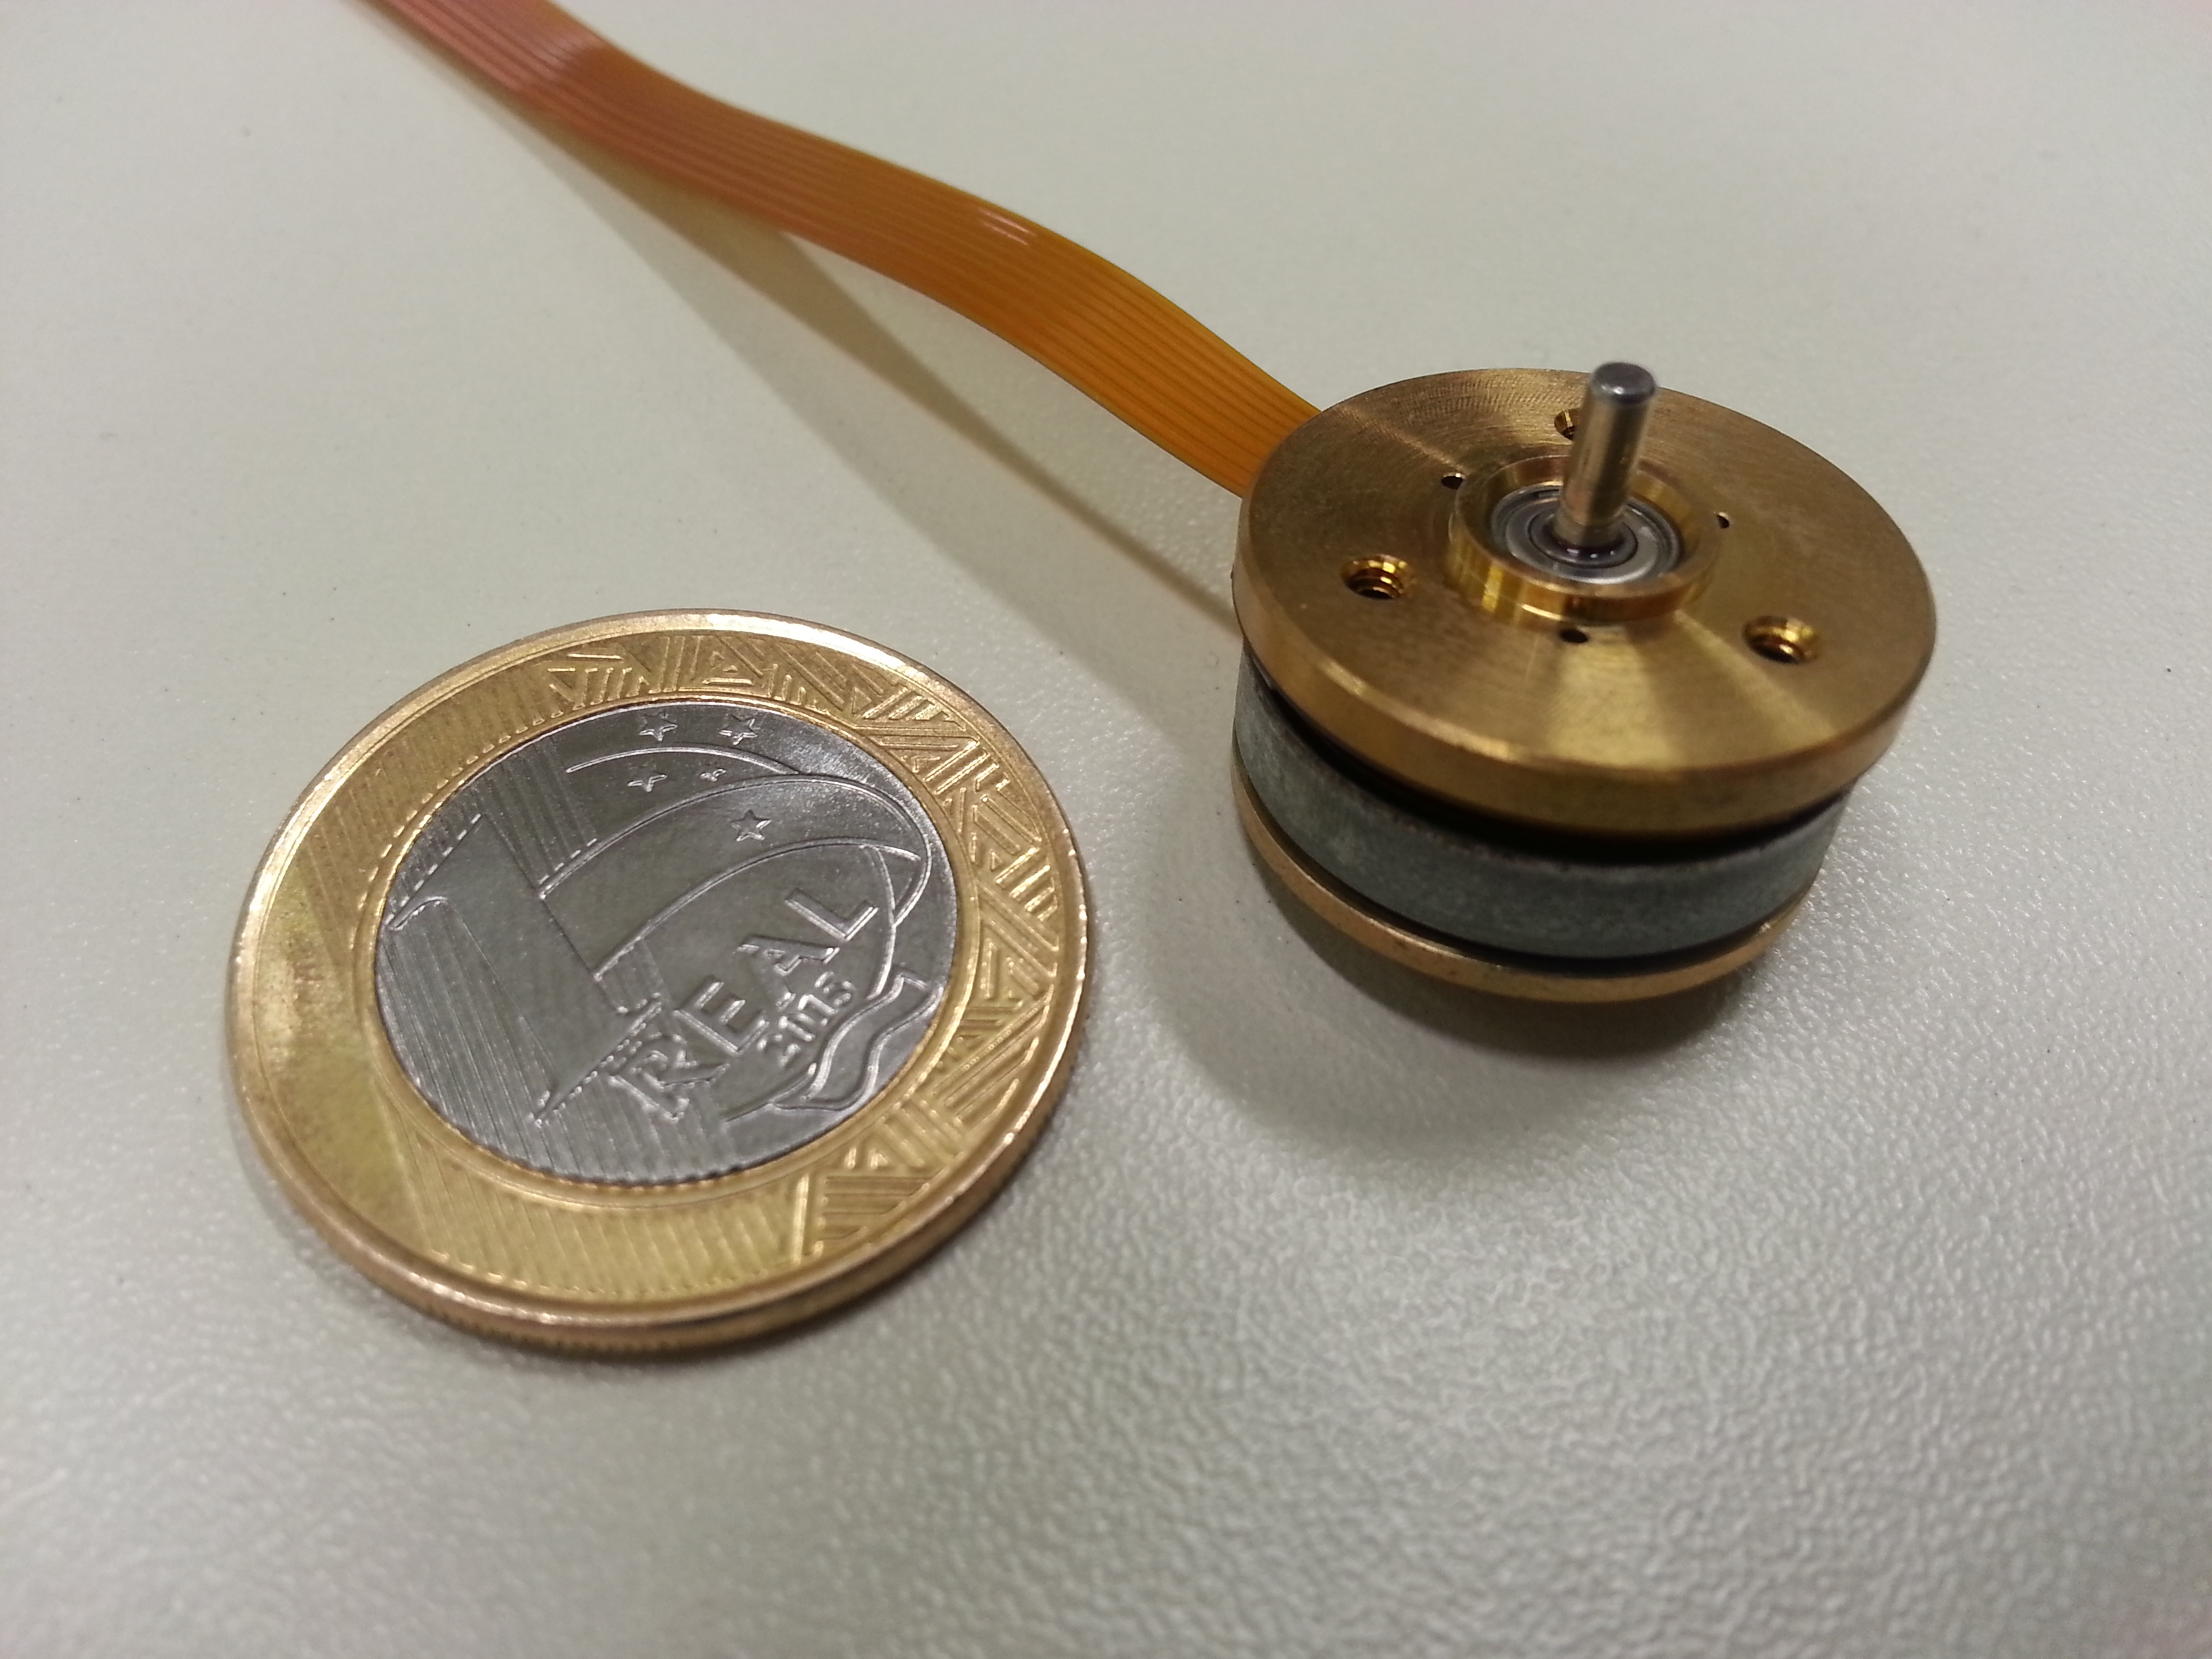
\includegraphics[width=0.6\linewidth]{./figs/Maxon_351100}
	
	\begin{small}
		FONTE: Arquivo dos autores.
	\end{small}
	\label{fig:Maxon}
\end{figure}

%\newpage

O motor que melhor atende a todos estes requisitos e portanto o utilizado neste trabalho é o motor \textit{brushless} modelo 351100 (Maxon, Suíça). O catálogo com as especificações técnicas deste motor encontram-se no Anexo \ref{an:MM}.

%O motor já estava definido e disponível no início do projeto pelo NSEE (Núcleo de Sistemas Eletrônicos Embarcados) como um dos objetivos do estudo, validando o uso de um motor \textit{brushless} de 3W.

\subsection{Rodas de reação}

A roda de reação é basicamente um disco rotativo com muita massa (em relação ao resto do sistema). Quanto maior a massa e a geometria dela, maior a inércia I(kgm$^{2}$), como demonstrado na Equação \ref{eq:Inercia}, onde m(kg) é a massa e r(m) é o raio da roda. A inércia cresce proporcionalmente ao quadrado o raio da roda.

\begin{equation}
I = \frac{m}{2} r^2
\label{eq:Inercia}
\end{equation}

A relação entre a massa da roda de reação com a massa do satélite influencia diretamente na forma como o controle é feito. Como dito anteriormente, quanto maior a massa da roda de reação, e consequentemente a inércia dele, maior a capacidade de atuação. Porém, dada a limitação de espaço hábil dentro do CubeSat, não é possível projetar uma roda de reação com raio grande. Para compensar, a roda utilizada deverá ter uma massa mais elevada, e a forma de conseguir isso com dimensões limitadas é utilizando materiais mais densos. Nesse caso, a roda foi projetada considerando aço, como mostrado a seguir na Figura \ref{fig:RW}.

\begin{figure}[th]
	\caption{Roda de reação.}
	\centering
	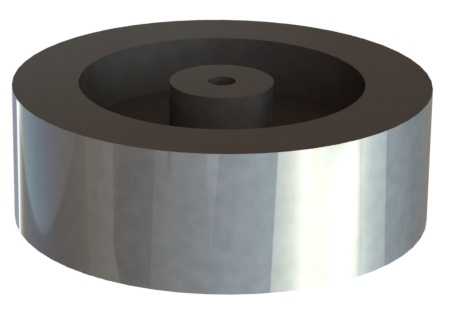
\includegraphics[width=0.5\linewidth]{./figs/Reaction_Wheel}
	
	\begin{small}
		FONTE: Arquivo dos autores.
	\end{small}
	\label{fig:RW}
\end{figure}

Por causa da forma como o motor é preso no suporte, foi necessário um pequeno rasgo na roda de reação com o objetivo de evitar que as cabeças dos parafusos interferissem na roda de reação, como mostrado nas folhas do projeto no Apêndice \ref{ap:RW}.

Apesar da roda projetada ser cilíndrica, ela não possui a mesma seção para toda sua extensão, e a Equação \ref{eq:Inercia} se aplica a corpos cilíndricos homogêneos. Para o cálculo correto da inercia, aplica-se a Equação \ref{eq:Inercia} para cada seção e então se aplica a equação \ref{eq:Inetot}.

\begin{equation}
I_{total} = \sum\nolimits I_{1} + I_{2} + I_{3}
\label{eq:Inetot}
\end{equation}

Serão usadas três rodas de reação, uma para cada motor. Elas foram usinadas em aço 1020, em um torno CNC. O peso delas ficou igual a 46g. A Inércia, portante, ficou igual a 57,44gcm$^{2}$. A inércia do rotor do motor é igual a 3,84gcm$^{2}$ (dado extraído do manual do motor, no Anexo \ref{an:MM}. Portanto, a inércia do conjunto ($I_{r}$) é igual a 61,28gcm$^{2}$ (ou 6,128$\cdot$10$^{-6}$kgm$^{2}$).

\subsection{Suporte do motor}

Para suportar o motor, foi desenvolvido um protótipo genérico obedecendo as furações dos motores e o espaço para o eixo para a fixação dos mesmos ao suporte e dele à placa de circuito eletrônico do CubeSat, como mostrado nas folhas do projeto no Apêndice \ref{ap:MS}. Esse suporte foi feito com altura de 10mm da superfície inferior do motor até a placa de circuito eletrônico para que não atrapalhasse o posicionamento dos componentes, como mostrado na Figura \ref{fig:MS} a seguir. Para atender aos requisitos de peso, o suporte foi projetado em alumínio.

\begin{figure}[th]
	\caption{Suporte do motor.}
	\centering
	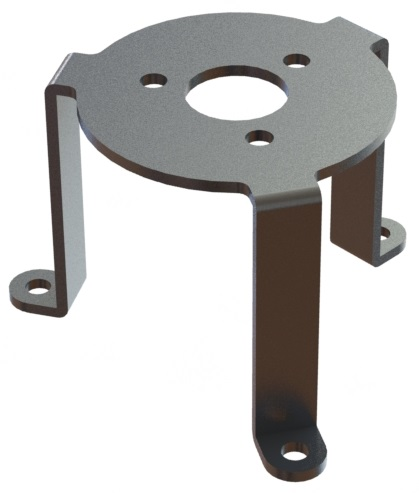
\includegraphics[width=0.45\linewidth]{./figs/Motor_Sup}
	
	\begin{small}
		FONTE: Arquivo dos autores.
	\end{small}
	\label{fig:MS}
\end{figure}

\newpage

São usados três suportes, um para cada motor. Eles foram fabricados com chapas de alumínio de 1mm de espessura através de uma máquina de corte a laser e então dobrados. O peso ficou igual a 2,3g.

\subsection{Estrutura mecânica}

A estrutura mecânica do CubeSat foi projetada seguindo os padrões indicados pela Cal Poly \cite{CalPoly}. O projeto foi feito pelo Núcleo de Sistemas Eletrônicos Embarcados (NSEE) da Mauá, que é responsável pelo desenvolvimento do CubeSat Mauá, sendo de nossa responsabilidade apenas o sistema de controle de atitude do satélite. O modelo básico sobre o qual o trabalho se desenvolveu é mostrado a seguir apenas com a estrutura mecânica em si a mostra na Figura \ref{fig:Frame}. %As folhas do projeto da estrutura mecânica se encontram no Anexo \ref{an:MS}.

\begin{figure}[th]
	\caption{Estrutura do CubeSat.}
	\centering
	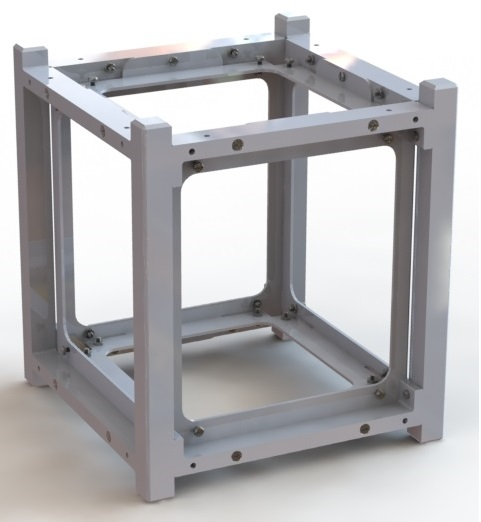
\includegraphics[width=0.5\linewidth]{./figs/Frame}
	
	\begin{small}
		FONTE: Arquivo dos autores.
	\end{small}
	\label{fig:Frame}
\end{figure}

\newpage

A estrutura mecânica é composta por uma estrutura principal, responsável por dar a forma e a sustentação do CubeSat e uma estrutura interna, responsável pela fixação das placas eletrônicas, ambas mostradas na Figura \ref{fig:Frame}. Há também chapas de fechamento externas que fecham e protegem o CubeSat, como mostrado a seguir na Figura \ref{fig:FrameFull}.

\begin{figure}[th]
	\caption{CubeSat montado.}
	\centering
	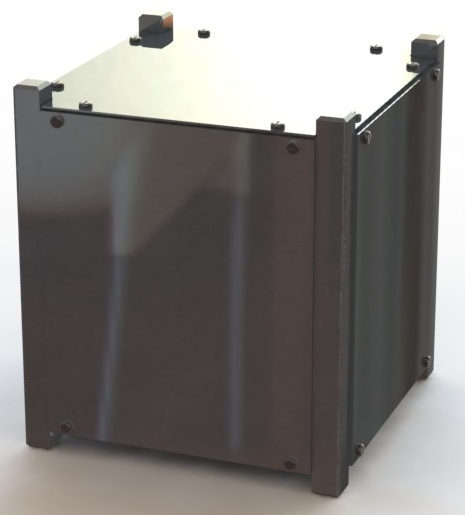
\includegraphics[width=0.5\linewidth]{./figs/Frame_Full}
	
	\begin{small}
		FONTE: Arquivo dos autores.
	\end{small}
	\label{fig:FrameFull}
\end{figure}

\newpage

A Tabela \ref{tab:MatMec} a seguir mostra quais os materiais necessários para a construção da estrutura mecânica do CubeSat. As folhas de projeto delas estão no Anexo \ref{an:MS}. Os elementos de fixação utilizados (inclusive os usados para a fixação das placas eletrônicas e suportes dos motores) também estão descritos na Tabela \ref{tab:MatMec}.

\begin{table}[h]
	\caption{Materiais para construção da estrutura mecânica do CubeSat.}
		\centering
	\begin{tabular}{|c|c|}
		\hline
		\textbf{Componentes} & \textbf{Quantidades} \\ 
		\hline 
		Estrutura Interna Lateral Principal & 2 \\ 
		\hline 
		Estrutura Interna Lateral de Ligação & 4 \\ 
		\hline 
		Estrutura Interna Superior & 2 \\
		\hline 
		Placa Interna Lateral & 8 \\
		\hline 
		Casca Externa Superior & 2 \\ 
		\hline 
		Casca Externa Lateral & 4 \\ 
		\hline 
		Parafuso Cabeça de Panela (Fenda) - M2 x 6mm & 105 \\
		\hline
		Porca Sextavada - M2 & 41 \\
		\hline
	\end{tabular}
	
	\begin{small}
	\vspace{3pt}	
	FONTE: Dos autores.
	\end{small}
	\label{tab:MatMec}
\end{table}

\chapter{Métodos}

Nesta seção, é explicada a metodologia aplicada para atingir os seguinte objetivos:

a)	desenvolver um sistema de controle de atitude para um satélite do tipo CubeSat, utilizando rodas de reação;

b)	desenvolver placas de circuitos eletrônicos que permitam a aquisição de dados de posicionamento, a comunicação entre micro controladores e o controle dos motores;

c)	desenvolver um \textit{firmware} que possa interpretar os dados de posicionamento e efetuar o controle de atitude.

\section{Base de teste}

Para que seja possível testar o CubeSat e avaliar se seu funcionamento é o esperado, foi desenvolvida uma base que fosse capaz de medir sua posição através de um \textit{encoder}.

\subsection{Estrutura}

A estrutura da base foi desenvolvida em alumínio, visando não adicionar influenciar na inércia do sistema. Ela é composta por quatro partes usinadas, desenvolvidas de forma que pudessem ser fabricadas facilmente. A base de teste é mostrada na Figura \ref{fig:ProtoTB}, a seguir.

\begin{figure}[th]
	\caption{Base de teste.}
	\centering
	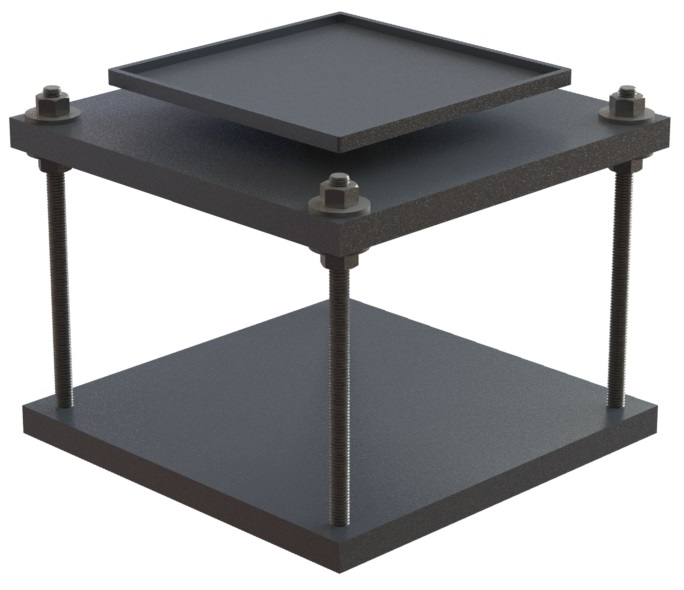
\includegraphics[width=0.6\linewidth]{./figs/Test_Base}
	
	\begin{small}
		FONTE: Arquivo dos autores.
	\end{small}
	\label{fig:ProtoTB}
\end{figure}

\newpage

A parte superior foi feita de forma que o CubeSat encaixe nela. Essa parte é acoplada em um eixo, apoiado sobre um rolamento axial de esferas 51100 (SKF, Cajamar, SP), e conectado na outra extremidade a um \textit{encoder}. O rolamento fica apoiado sobre o restante da estrutura que serve tanto para sustentar todo o sistema quanto dar apoio ao \textit{encoder} e à placa que adquire seus dados. As hastes de sustentação da estrutura são barras roscadas M6, que permitem um nivelamento da base sobre qualquer superfície, garantindo que a medição fique livre de interferências. A seguir, na Tabela \ref{tab:MatTB}, a lista de materiais necessários para fabricação e montagem da base de testes.

\begin{table}[h]
	\caption{Materiais para construção da estrutura mecânica da base de testes do CubeSat.}
		\centering
	\begin{tabular}{|c|c|}
		\hline
		\textbf{Componentes} & \textbf{Quantidades} \\ 
		\hline 
		Suporte do CubeSat & 1 \\ 
		\hline 
		Eixo & 1 \\
		\hline
		Base Superior & 1 \\ 
		\hline 
		Base Inferior & 1 \\
		\hline 
		Barra Roscada - M6 x 120mm & 4 \\
		\hline 
		Arruela - M6 & 8 \\ 
		\hline 
		Porca Sextavada - M6 & 8 \\ 
		\hline 
		Rolamento Axial - SKF 51100 & 1 \\
		\hline
	\end{tabular}
	
	\begin{small}
	\vspace{3pt}	
	FONTE: Dos autores.
	\end{small}
	\label{tab:MatTB}
\end{table}

O rolamento foi dimensionado de forma que tivesse uma vida virtualmente infinita (muito grande), mas que não fosse muito grande para não influenciar na inércia do sistema. O rolamento mencionado anteriormente possui diâmetro interno de 10mm, o menor disponível. Para verificar sua vida útil, foi usada a Equação \ref{eq:RolVida} a seguir \cite{ProjMaq}.

\begin{equation}
L_{h} = \frac{ \left( \frac{C}{P} \right)^{p} 10^{6}}{\frac{\omega \cdot 60^{2}}{2 \pi}}
\label{eq:RolVida}
\end{equation}

Onde L$_{h}$ é a vida em horas, C (N) é a classificação de carga básica dinâmica do rolamento, P (N) é a força aplicada sobre ele, p é o coeficiente de ajuste de acordo com o tipo de rolamento e $\omega$(rad/s) é a velocidade angular imposta sobre o rolamento.

Considerando que o peso do CubeSat é de 0,631kg, C é igual a 9950N, p é igual a 3 e a velocidade de rotação média de um CubeSat é aproximadamente 4,8rad/s, esses valores são substituídos e calculados, resultando em:

%\begin{equation}
\begin{center}
$L_{h} = \frac{ \left( \frac{9950}{0,639 \cdot 9,807 } \right)^{3} 10^{6}}{\frac{4,8 \cdot 60^{2}}{2 \pi}} \Longrightarrow Lh = 1,512 \cdot 10^{12} h$
\end{center}
%\label{eq:RolVidaRes}
%\end{equation}

Este alto valor de horas mostra que a vida do rolamento é de fato infinita, principalmente quando se considera que o rolamento não trabalhará com rotações completas sempre. Na maioria dos casos, dará apenas frações de voltas.

Para o dimensionamento das barras roscadas, foi-se adotado que seriam de tamanho M6 (6mm de diâmetro), com o objetivo de prender o sistema de maneira firme, mas que pudesse ser ajustado no caso de superfícies desniveladas. Para garantir que elas suportariam, foi feito um teste de flambagem onde se usou a Equação \ref{eq:Flamb} a seguir \cite{ProjMaq}.

\begin{equation}
d_{h} = \sqrt[4]{ \frac{64 \cdot Cs \cdot \lambda^{2} \cdot Fp \cdot \varphi }{ \pi^{3} \cdot E } }
\label{eq:Flamb}
\end{equation}

Onde Cs é o coeficiente de segurança (adotado como 5), $\lambda$ é o coeficiente de flambagem que, no caso, equivale ao dobro do comprimento da barra já que ela é engastada na base, F$_{p}$ (N) é a Força de projeto, $\varphi$ é o fator de ajuste (adotado como 1,5) e E (MPa) é o módulo de elasticidade do material, no caso um aço inoxidável com módulo igual a 193 GPa. No caso da Força, como a base é simétrica vertical e horizontalmente, o centro de massa fica equidistante dos quatro apoios. A força aplicada então é dividida igualmente por quatro:

%\begin{equation}
\begin{center}
$F_{p} = \frac{1,310 \cdot 9,807}{4} = 3,212 N$
\end{center}
%\label{eq:Fp}
%\end{equation}

Substituindo os valores na Equação \ref{eq:Flamb}, obtemos:

%\begin{equation}
\begin{center}
$d_{h} = \sqrt[4]{ \frac{64 \cdot 5 \cdot 240^{2} \cdot 3,212 \cdot 1,5 }{ \pi^{3} \cdot 210000 } } \Longrightarrow dh = 1,922 mm$
\end{center}
%\label{eq:FlambRes}
%\end{equation}

Como o eixo adotado possui diâmetro de 6mm, ele é maior que o diâmetro mínimo necessário para suportar a carga e portanto não ocorre flambagem.

Os desenhos de projeto das partes da base estão no Apêndice \ref{ap:TB}. A Figura \ref{fig:ProtoTBOK}, a seguir, mostra como ficou a base de teste.

\begin{figure}[th]
	\caption{Base de teste pronta}
	\centering
	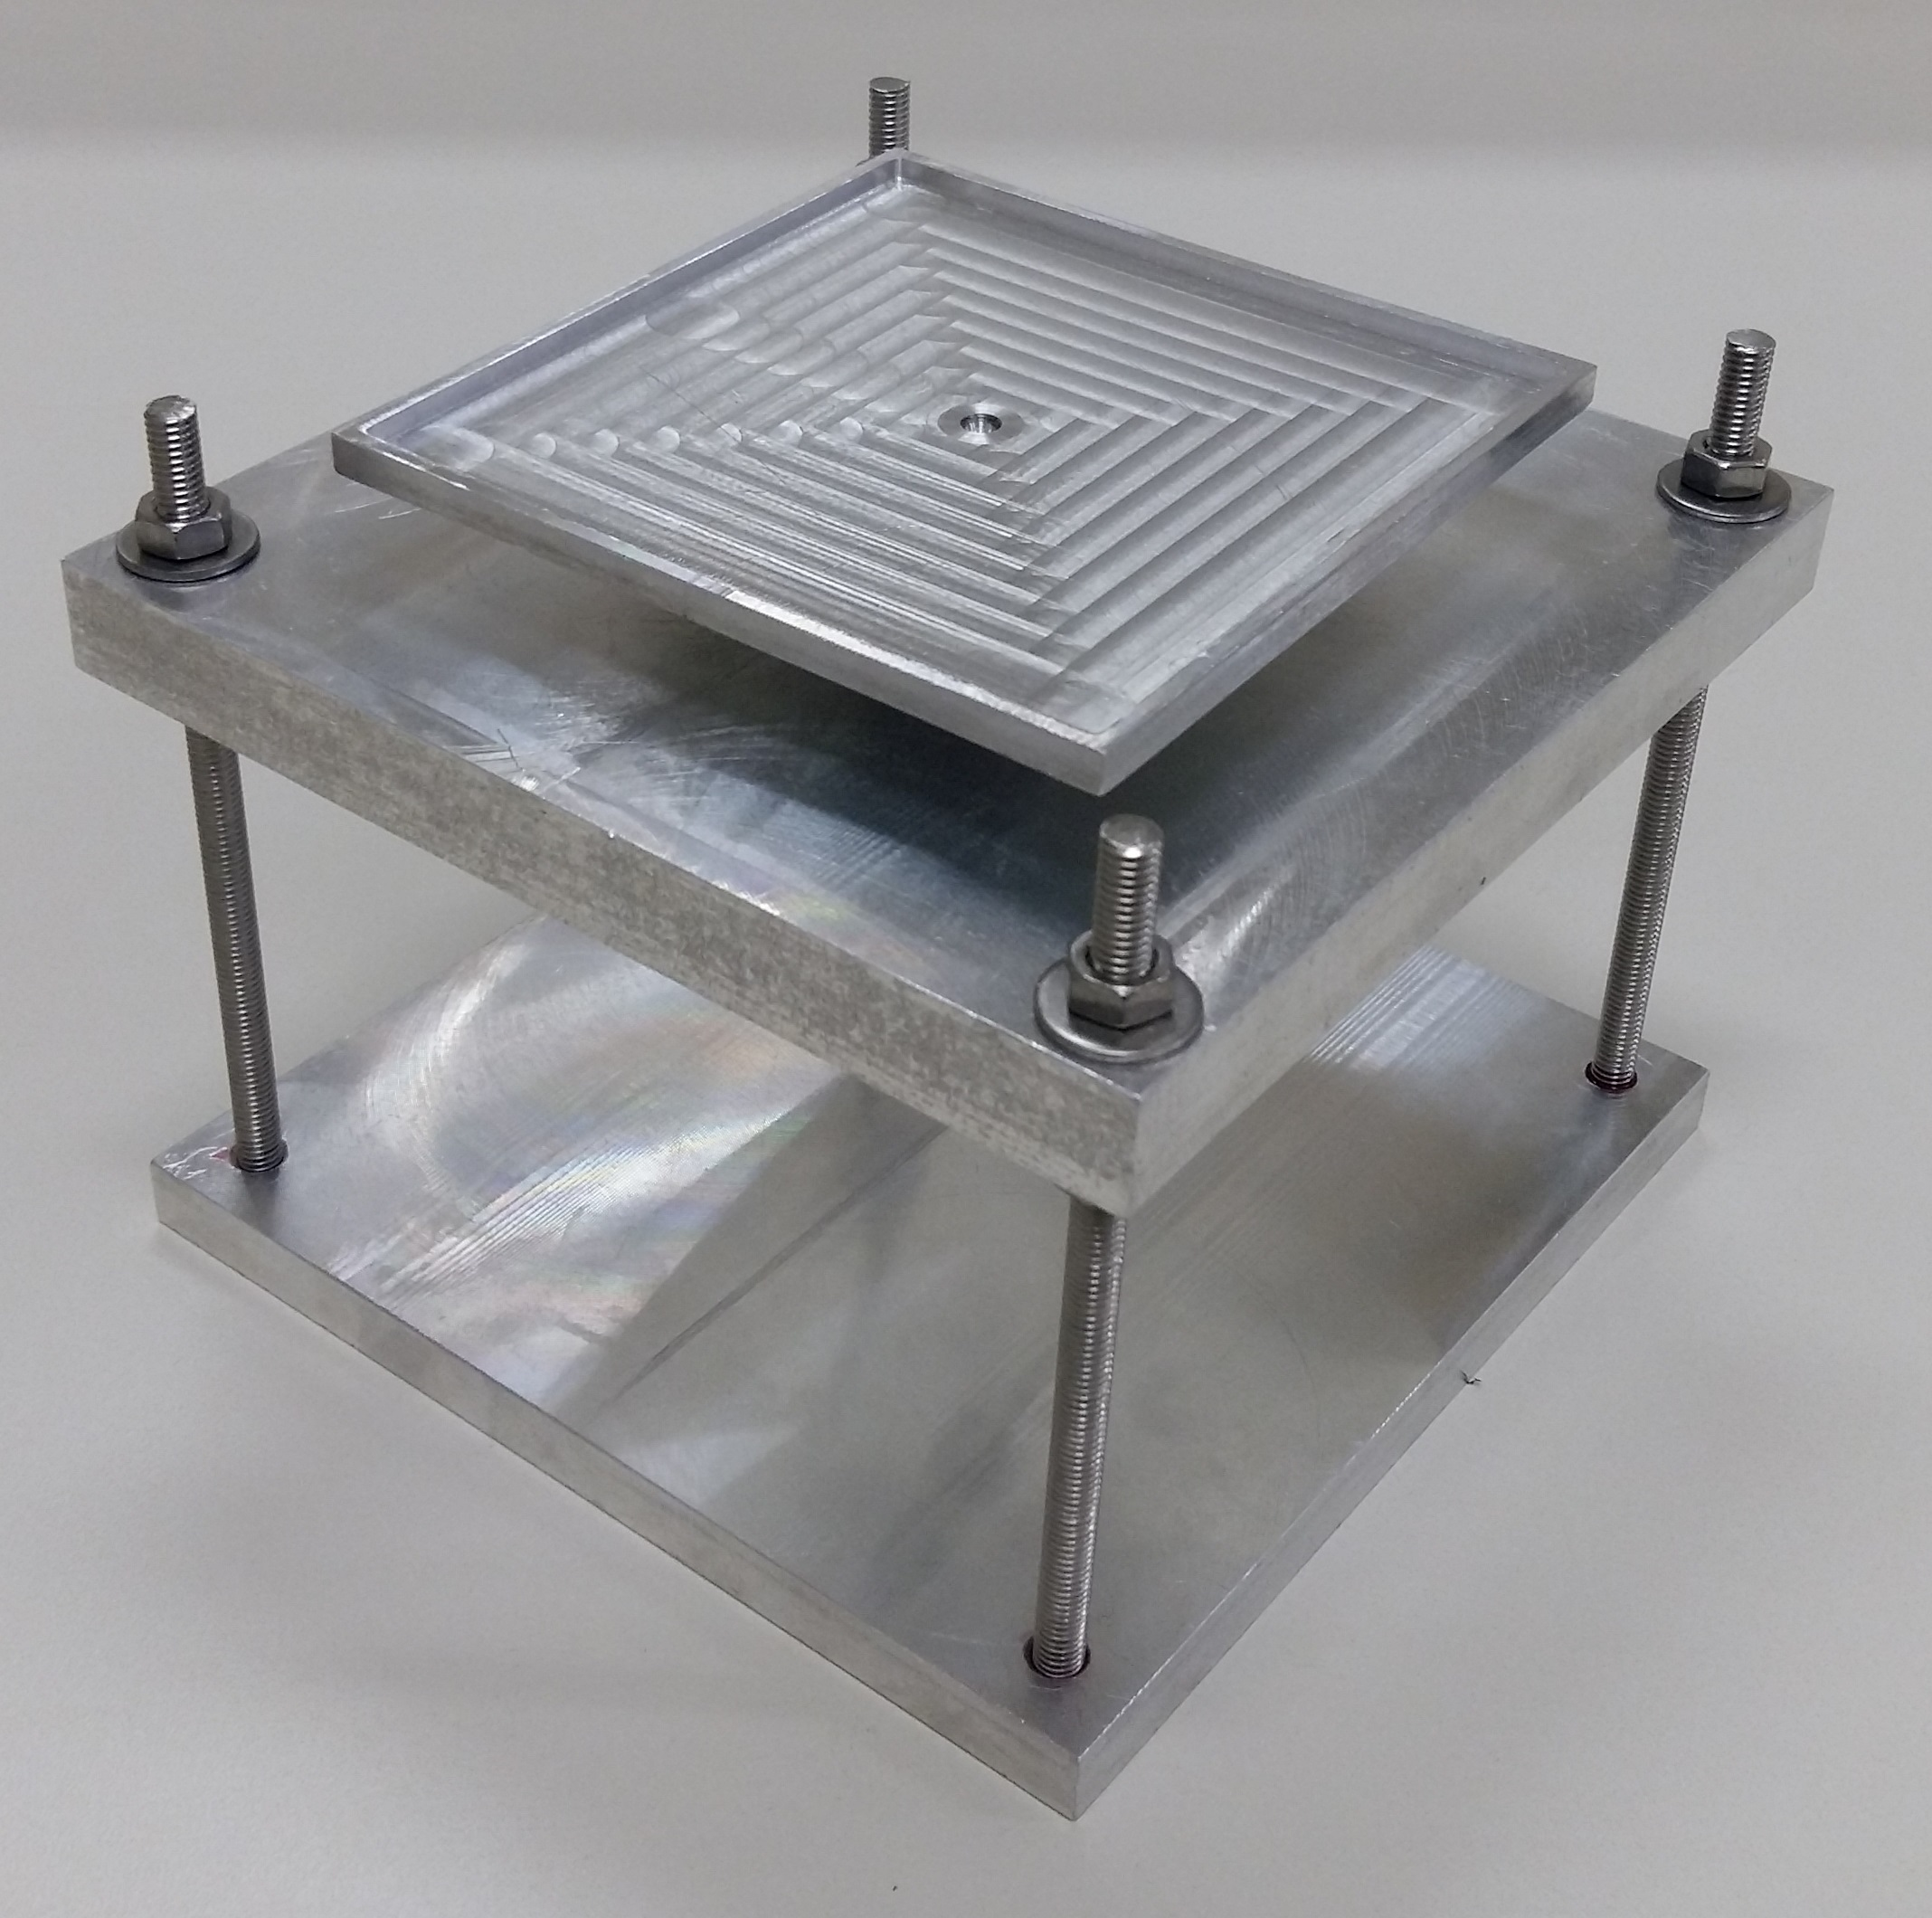
\includegraphics[width=0.6\linewidth]{./figs/Test_Base_Proto}
	
	\begin{small}
		FONTE: Arquivo dos autores.
	\end{small}
	\label{fig:ProtoTBOK}
\end{figure}

\newpage

\subsection{Encoder}



\section{Modelagem e controle}

A modelagem do CubeSat foi feita para que pudessem ser conhecidas as equações que regem o sistema como um todo. As equações se resumem nas equações de dinâmica da roda de reação junto do motor (subsistema) e na dinâmica do CubeSat (sistema).

\subsection{Roda de reação e motor}

Ao aplicar uma tensão V (V) em um motor elétrico, uma corrente i (A) passará pelos enrolamentos dele e será convertida em um torque mecânico T$_{m}$ (kgm$^{2}$/s$^{2}$). No motor, há uma resistência R ($\Omega$) devido aos enrolamentos das bobinas. É nessas bobinas que a corrente induz um campo magnético que força o eixo do motor a girar. Isso gera uma tensão contra-eletromotriz V$_{emf}$ (V), que é mostrada na Equação \ref{eq:Tens}.

\begin{equation}
V = i R + V_{emf}
\label{eq:Tens}
\end{equation}

A relação de um motor com imã permanente entre a corrente, o torque T$_{m}$ (Nm) e a constante de torque k$_{T}$ (Nm/A) é descrita na Equação \ref{eq:Torq},  .

\begin{equation}
T_{m} = k_{T} i
\label{eq:Torq}
\end{equation}

A queda de tensão no motor resulta em uma perda de potência. Essa perda costuma ser pequena (e portanto desprezada) caso o motor esteja em boas condições e sem nenhum defeito. O V$_{emf}$ pode ser descrito como na Equação \ref{eq:Vemf}, onde k$_{T}$ e k$_{E}$ (Vs/rad) são o mesmo para um motor com 100\% de eficiência.

\begin{equation}
V_{emf} = k_{T} \omega_{r} = k_{E} \omega_{r}
\label{eq:Vemf}
\end{equation}

Aproveitando a equação de dinâmica da roda de reação, temos a Equação \ref{eq:Tm}, onde $I_{r}$ é o total de inércia do motor junto da roda de reação, B é o coeficiente de atrito viscoso e $\dot{\omega}_{r}$ é a aceleração angular.

\begin{equation}
T_{m} = I_{r} \dot{\omega}_{r} + B \omega_{r}
\label{eq:Tm}
\end{equation}

A Equação \ref{eq:Tens} é substituída na equação \ref{eq:Torq} e substituindo o $V_{emf}$ pela equação \ref{eq:Vemf}, obtemos uma expressão que é igual à Equação \ref{eq:Tm}, como mostrado a seguir:

\begin{align}
	T_{m} & = k_{T} i \nonumber \\
	& = k_{T} \frac{V - V_{emf}}{R} \nonumber \\
	& = k_{T} \frac{ V - k_{T} \omega_{r} }{R} = I_{r} \dot{\omega}_{r} + B \omega_{r}
\label{eq:Subst}
\end{align}

Reescrevendo:

\begin{equation}
I_{r} \dot{\omega}_{r} + \left( B + \frac{k_{T}^{2}}{R} \right) \omega_{r} = \frac{k_{T}}{R} V \nonumber
\label{eq:ReWrite}
\end{equation}

Aplicando então a transformada de Laplace e isolando os termos de saída sobre entrada, obtém-se:

\begin{equation}
\frac{\Omega_{r}(s)}{V(s)} = \frac{\frac{1}{B R + k_{T}}}{\frac{I_{r} R}{B R + k_{T}^{2}} s +1}
\label{eq:Lap}
\end{equation}

Da Equação \ref{eq:Lap}, é possível observar que o valor do denominador e o que multiplica o s são constantes. Portanto, a equação pode ser reescrita da seguinte forma:

\begin{equation}
\frac{\Omega_{r}(s)}{V(s)} = \frac{k_{r}}{\tau_{r} s +1}
\label{eq:RWDM}
\end{equation}

Onde $k_{r}$ e $\tau_{r}$ são constantes. Portanto, a Equação \ref{eq:RWDM} é o modelo dinâmico do conjunto roda de reação e motor escritos \cite{Ericksson}.

Para fazer a equação de controle do sistema modelado anteriormente, foi consideradoo seguinte funcionamento: a entrada do sistema é um \textit{set point} de velocidade angular que é subtraído pela realimentação, gerando um erro que entra no controlador K$_{r}$ e sai como uma tensão (V), que por sua vez entra na planta G$_{r}$ e resulta em uma velocidade angular, fechando a malha. Isso tudo é mostrado a seguir, na Figura \ref{fig:Diagram}.

\begin{figure}[th]
	\caption{Diagrama de blocos do sistema motor e roda de reação.}
	\centering
	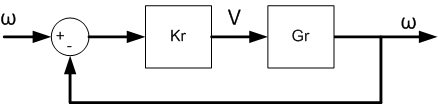
\includegraphics[width=0.7\linewidth]{./figs/Motor_Subsystem}
	
	\begin{small}
		FONTE: Arquivo dos autores.
	\end{small}
	\label{fig:Diagram}
\end{figure}

Observando a equação da planta, chegou-se a conclusão de que um controlador Proporcional-Integral (PI) seria o mais adequado. Portanto, tomou-se como base a Equação \ref{eq:PI} a seguir:

\begin{equation}
K_{r}(s) = \frac{k_{cr}(s+z_{r0})}{s}
\label{eq:PI}
\end{equation}

Onde k$_{cr}$ é o ganho do controlador e z$_{r0}$ é o zero do controlador. Para calcular os valores das constantes, precisou-se determinar o valor de k$_{r}$ e $\tau_{r}$, dependentes de constantes já conhecidas: I$_{r}$ = 6,128$\cdot$10$^{-6}$ kgm$^{2}$, R = 23,9 $\Omega$, k$_{T}$ = 11,3$\cdot$10$^{-3}$ Nm/A e B = 4,9$\cdot$10$^{-6}$ kgm$^{2}$/s. A inércia foi obtida através do \textit{software} de simulação SolidWorks 2013 e validados comparando a massa obtida através dele com a massa real. A resistência e a constante de torque foi obtida no catálogo do motor, no Anexo \ref{an:MM}. Já o coeficiente de atrito viscoso foi estimado com referência à testes realizados no INPE \cite{Carrara}. Com estes valores, calculou-se que k$_{r}$ = 87,588 e $\tau_{r}$ = 0,598.

Com estes valores, o controlador foi projetado de forma que o zero "cancelasse" o polo da planta, portanto: z$_{r0}$ = 0,598. Já o ganho foi igualado a 2 dividido pelo ganho da planta, para que o ganho final seja igual a 2. Logo:

\begin{equation}
k_{cr} = 2/87,588 \Longrightarrow k_{cr} = 0,022834 \nonumber
\label{eq:kcr}
\end{equation}

Substituindo os valores encontrados na Equação \ref{eq:PI}, obtemos:

\begin{equation}
K_{r}(s) = \frac{0,022834(s+0,598)}{s}
\label{eq:PI_calc}
\end{equation}

Discretizando a Equação \ref{eq:PI_calc} no \textit{software} matemático MATLAB com período de amostragem T =  s, através do método de Tustin, obteve-se a equação:

\begin{equation}
K_{r}(z) = \frac{0,023107314300773-0,022561042095081}{z-1}
\label{eq:PI_disc}
\end{equation}

Da Equação \ref{eq:PI_disc}, obtém-se a equação de diferenças implementada no microcontrolador:

\begin{equation}
u_{rk} = u_{rk-1} + 0,023107314300773e_{rk} - 0,022561042095081e_{rk-1}
\label{eq:PI_eqdif}
\end{equation}

O elevado número de casas decimais é devido ao fato dos valores serem muito próximos entre si, podendo levar a uma diferença de erros muito pequena, causando um erro estacionário.

\subsection{CubeSat}

O satélite será afetado pela rotação dos conjuntos motor - roda de reação. Pela terceira Lei de Newton, o momento torçor que age no conjunto reage no sistema, criando um momento torçor de igual intensidade no sentido contrário, como mostrado na Equação \ref{eq:Newton}.

\begin{equation}
M_{r} = M
\label{eq:Newton}
\end{equation}

Onde $M_{r}$ é o momento torçor do conjunto e M é o momento torçor do sistema. Pode-se considerar que a dinâmica do sistema é composta unicamente por uma inércia sujeita a um torque resistivo causado por um coeficiente de atrito seco com o ar. Ou seja, $M_{r}$ é causado pela inércia da roda de reação somada com a inércia do rotor do motor $I_{r}$ multiplicados pela aceleração angular $\dot{\omega}_{r}$. Enquanto M é a inércia do satélite I multiplicado pela aceleração do sistema $\dot{\omega}$,  decrescido do coeficiente de atrito C multiplicado pela velocidade angular $\omega$. Isso é demonstrado a seguir, na Equação \ref{eq:Moment}.

\begin{equation}
I_{r}\dot{\omega}_{w} = I\dot{\omega} - C\omega
\label{eq:Moment}
\end{equation}

Reorganizando a equação, aplicando Laplace e isolando os termos de entrada (velocidade da roda de reação) sobre a saída (velocidade do satélite), obtemos a Equação \ref{eq:LapMom} mostrada a seguir.

\begin{equation}
\frac{\Omega(s)}{\Omega(s)_{r}} = \frac{I_{r}s}{Is - C}
\label{eq:LapMom}
\end{equation}

Ao colocar um integrador na saída do sistema, obtemos a posição dele, que é a variável a ser controlada. Isso significa que a Equação \ref{eq:SDM} a seguir é o modelo dinâmico do sistema.

\begin{equation}
\frac{\Theta(s)}{\Omega(s)_{r}} = \frac{I_{r}}{Is - C}
\label{eq:SDM}
\end{equation}

%\includegraphics[width=.8\linewidth]{untitled.eps}

% ----------------------------------------------------------
% PROTÓTIPO 
% ----------------------------------------------------------
\chapter{Protótipo}

Nesta seção está a descrição de como foi feito o protótipo do CubeSat. Desde os elementos individuais, como as rodas de reação, suportes dos motores, estruturas mecânicas e placas eletrônicas, até o CubeSat como um todo.

\section{Rodas de reação}

Os protótipos das rodas de reação foram feitos em aço 1020 em um torno CNC (Baron-Max, Taiwan) pela empresa Rudloff. A seguir, na Figura \ref{fig:ProtoRW}, uma imagem de como ficaram.

\begin{figure}[th]
	\caption{Modelo das rodas de reação.}
	\centering
	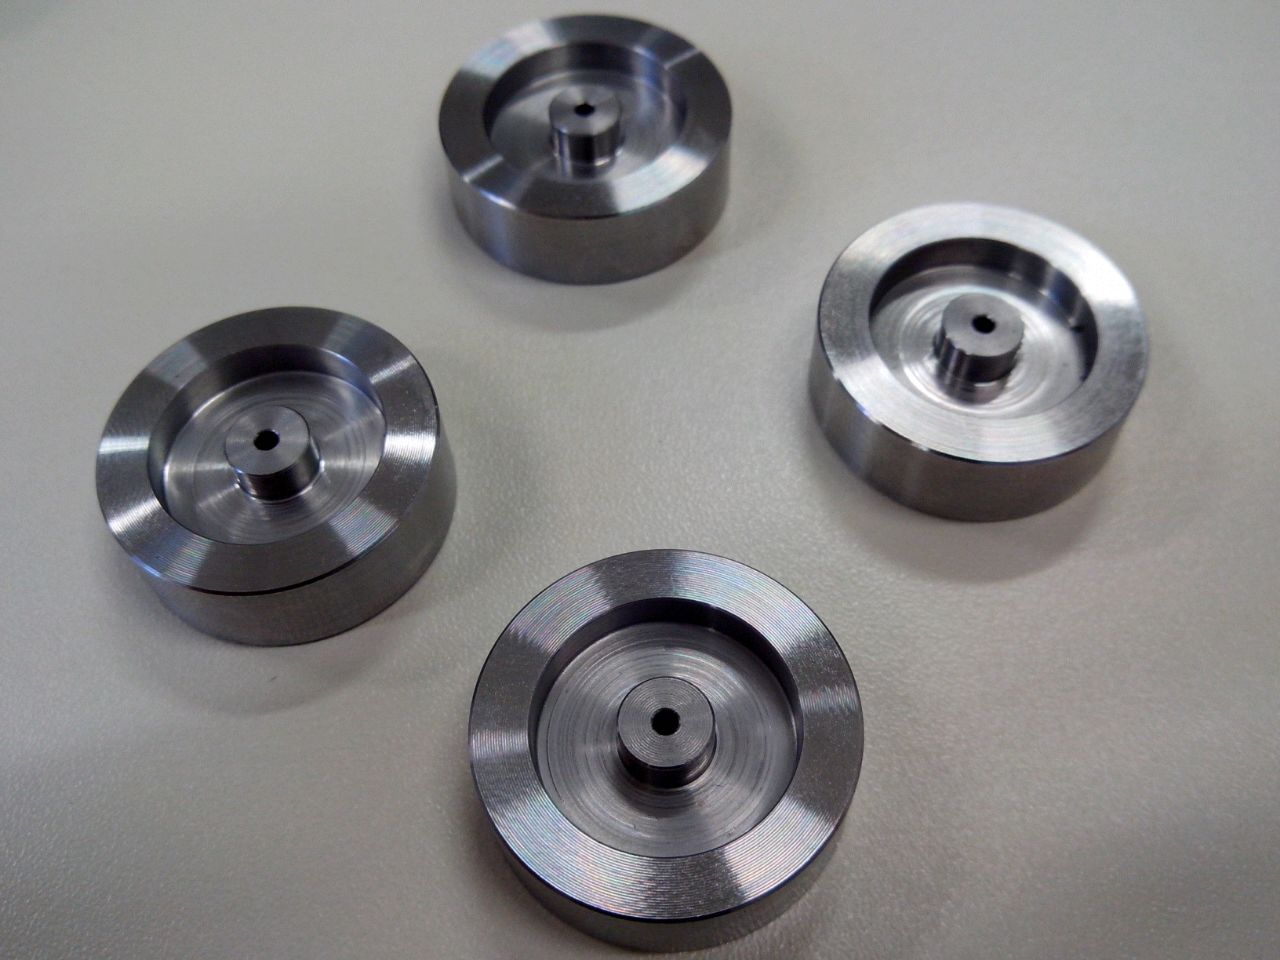
\includegraphics[width=0.7\linewidth]{./figs/Proto_RW}
	
	\begin{small}
		FONTE: Arquivo dos autores.
	\end{small}
	\label{fig:ProtoRW}
\end{figure}

\section{Suporte do motor}

Para uma pré validação do projeto do suporte do motor, foi feito um modelo impresso em uma impressora 3D (Cliever, Porto Alegre, RS), como mostrado a seguir na Figura \ref{fig:ProtoMSP}. Esse modelo foi usado para garantir o batimento dos furos do suporte com os do motor.

\begin{figure}[th]
	\caption{Protótipo em resina do suporte do motor.}
	\centering
	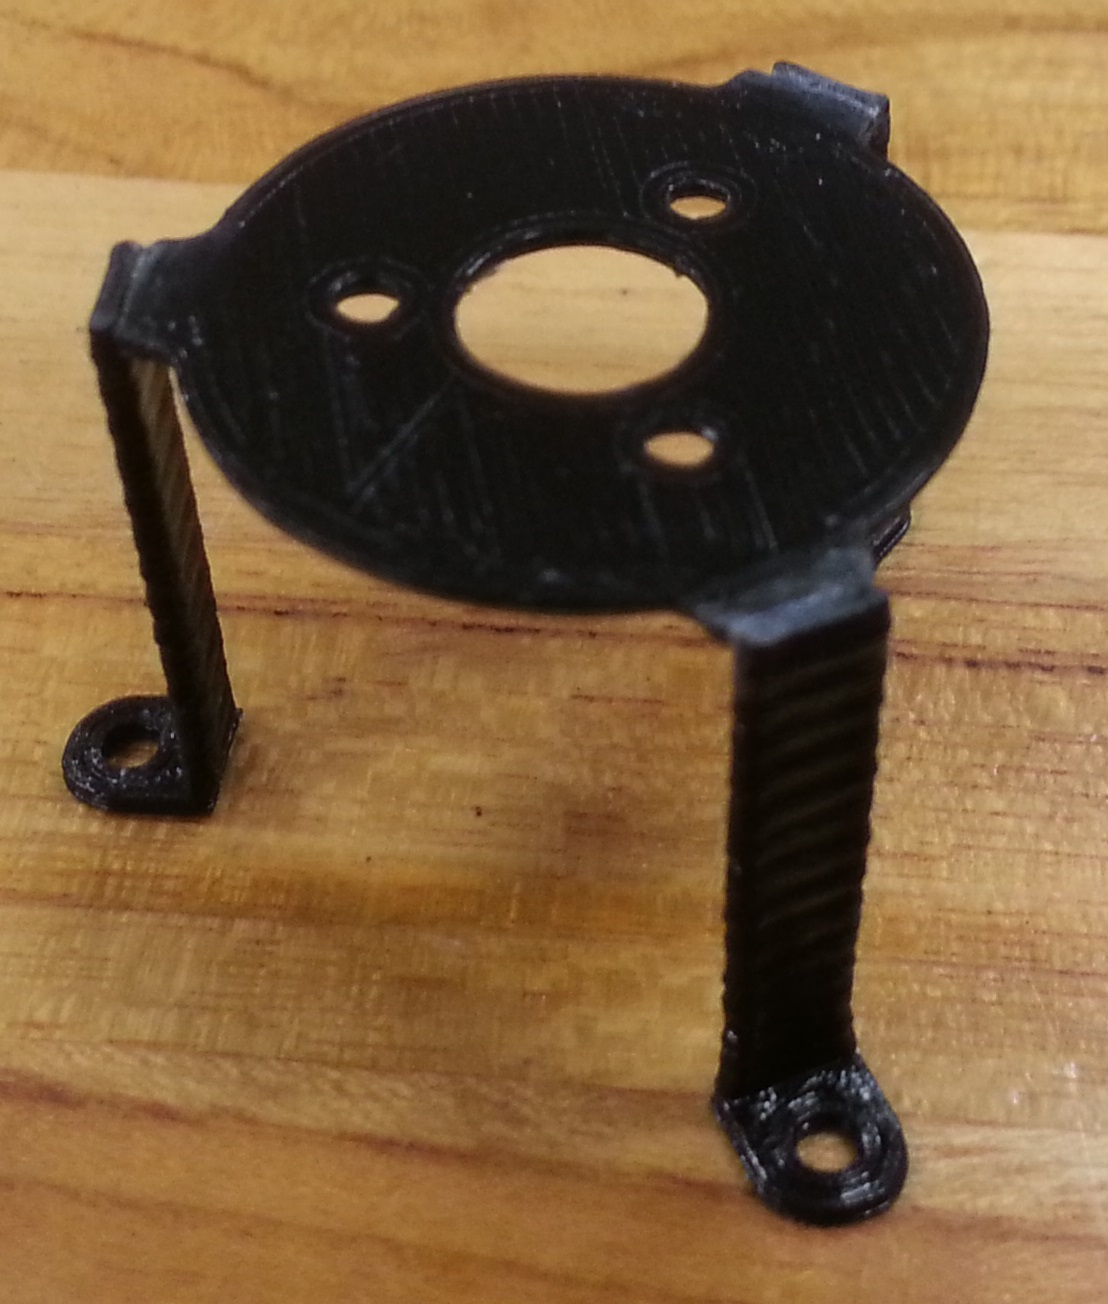
\includegraphics[width=0.5\linewidth]{./figs/Proto_3D}
	
	\begin{small}
		FONTE: Arquivo dos autores.
	\end{small}
	\label{fig:ProtoMSP}
\end{figure}

\newpage

Uma vez validado, foi mandado fazer um modelo em alumínio, através do corte por máquina de corte laser (Bystronic, Suíça) e dobra, através de uma dobradeira (Bystronic, Suíça). Esse modelo é mostrado a seguir, na Figura \ref{fig:ProtoMS}.

\begin{figure}[th]
	\caption{Modelo em metal do suporte do motor.}
	\centering
	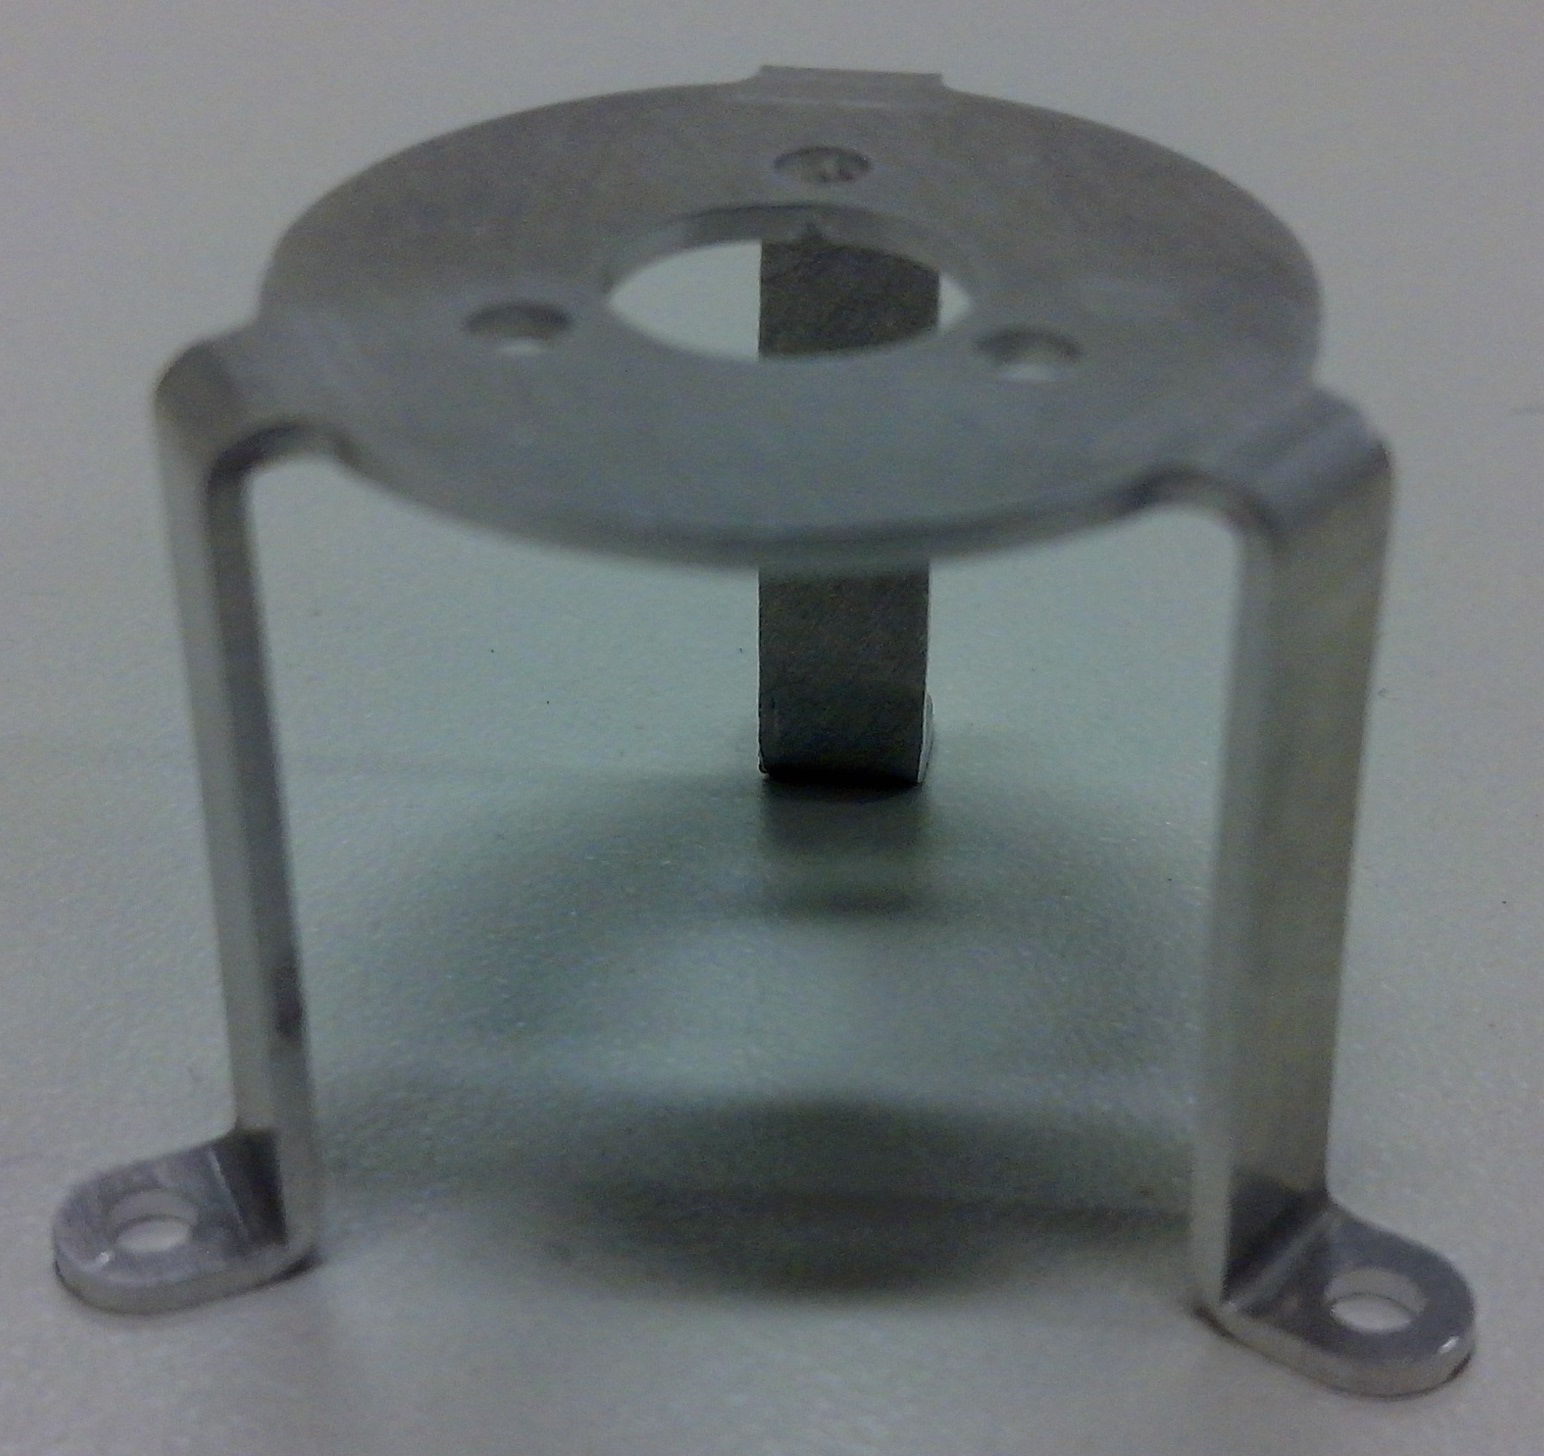
\includegraphics[width=0.5\linewidth]{./figs/Proto_MS}
	
	\begin{small}
		FONTE: Arquivo dos autores.
	\end{small}
	\label{fig:ProtoMS}
\end{figure}

\section{Estrutura mecânica}

Um primeiro protótipo da estrutura mecânica foi fabricado na oficina mecânica da Mauá para que pudessem ser feitos os primeiros testes de encaixe, tanto da própria estrutura quanto das placas de circuito eletrônico, inteira em alumínio. A seguir, na Figura \ref{fig:Protoone}, a estrutura montada. Foram deixadas três chapas de fechamento removidas para que fosse possível visualizar o interior do mesmo.

\begin{figure}[ht]
	\caption{Primeiro protótipo do CubeSat com três chapas de fechamento removidas.}
	\centering
	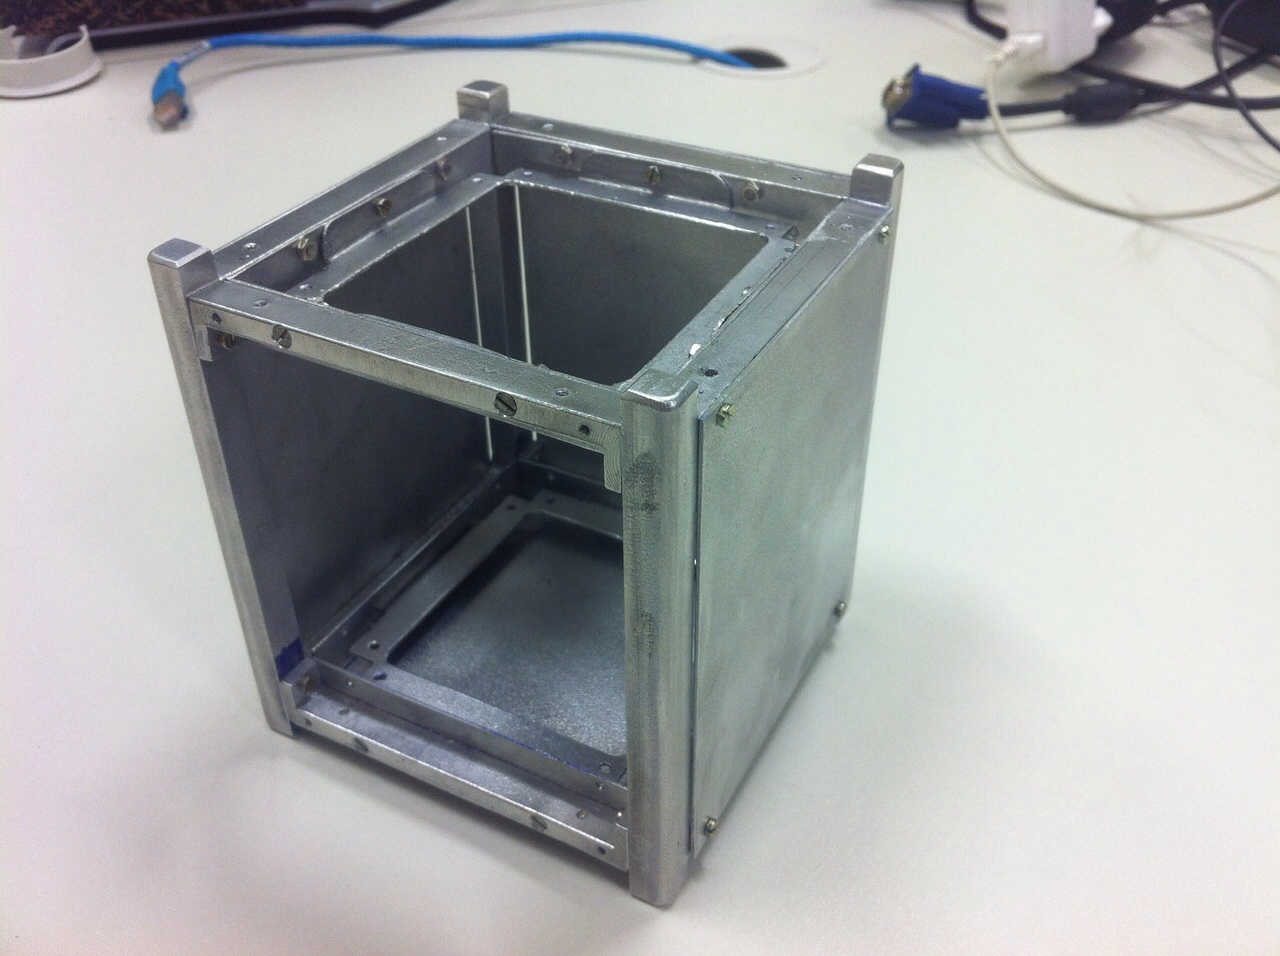
\includegraphics[width=0.6\linewidth]{./figs/PrototypeOne}
	
	\begin{small}
		FONTE: Arquivo dos autores.
	\end{small}
	\label{fig:Protoone}
\end{figure}

%\newpage

Posteriormente, foram feitos ajustes nos desenhos em CAD e uma nova versão foi feita. As partes de chapas foram feitas em máquinas de corte laser e dobradas, caso necessário, por uma empresa especializada. As outras partes foram feitas em um centro de usinagem no laboratório de usinagem da Mauá. O modelo finalizado sem as chapas de fechamento é mostrado a seguir, na Figura \ref{fig:ProtoTwo}.

\begin{figure}[th]
	\caption{Versão final da estrutura do CubeSat.}
	\centering
%	\includegraphics[width=0.7\linewidth]{./figs/}
	
	\begin{small}
		FONTE: Arquivo dos autores.
	\end{small}
	\label{fig:ProtoTwo}
\end{figure}

\section{Placas eletrônicas}



% ----------------------------------------------------------
% RESULTADOS E DISCUSSÕES
% ----------------------------------------------------------
\chapter{Resultados e discussões}

% ----------------------------------------------------------
% CONCLUSÕES
% ----------------------------------------------------------
\chapter{Conclusões}

% ----------------------------------------------------------
% REFERÊNCIAS BIBLIOGRÁFICAS
% ----------------------------------------------------------
\bibliography{TCC_Sist_Controle_Atitude}

% ----------------------------------------------------------
% Apêndices
% ----------------------------------------------------------
% Inicia os apêndices
% ---
\begin{apendicesenv}
% Imprime uma página indicando o início dos apêndices
\partapendices
% ---

\chapter{Desenho da placa de controle}

\begin{figure}[th]
	\centering
	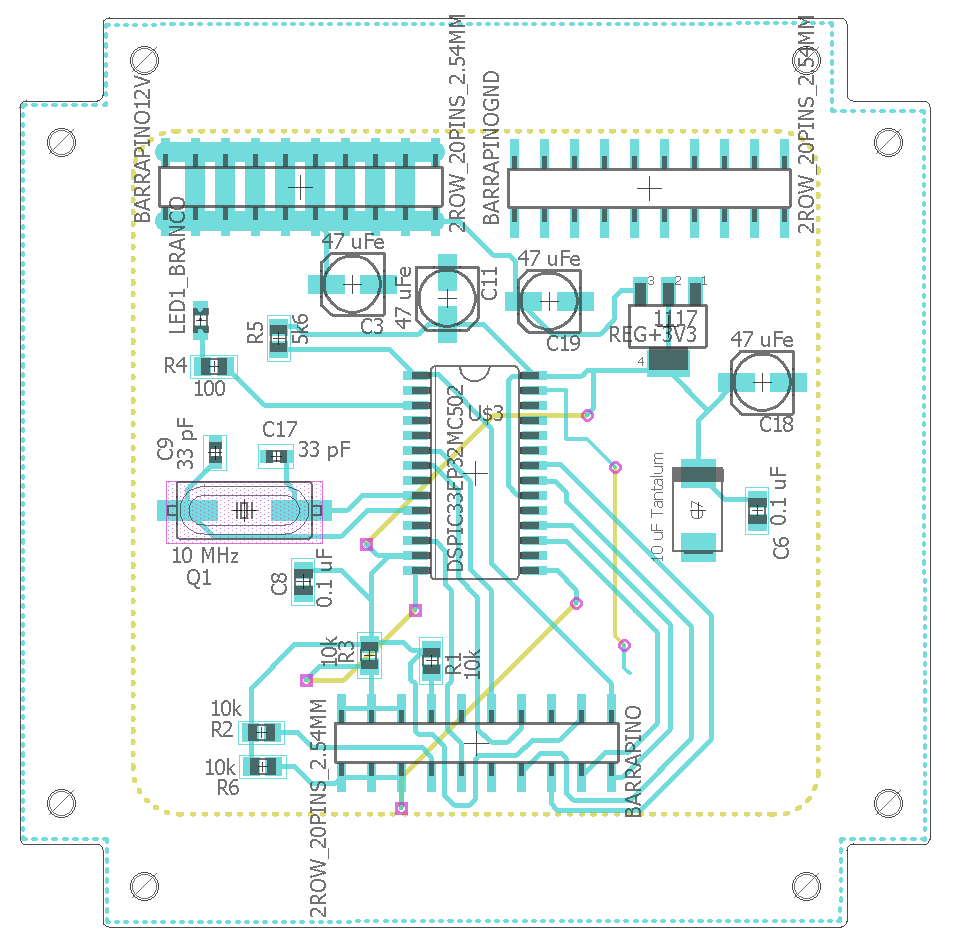
\includegraphics[width=1\linewidth]{./figs/Placa_master}
\end{figure}

\label{ap:PMaster}

\chapter{Desenho da placa dos motores}

\begin{figure}[th]
	\centering
	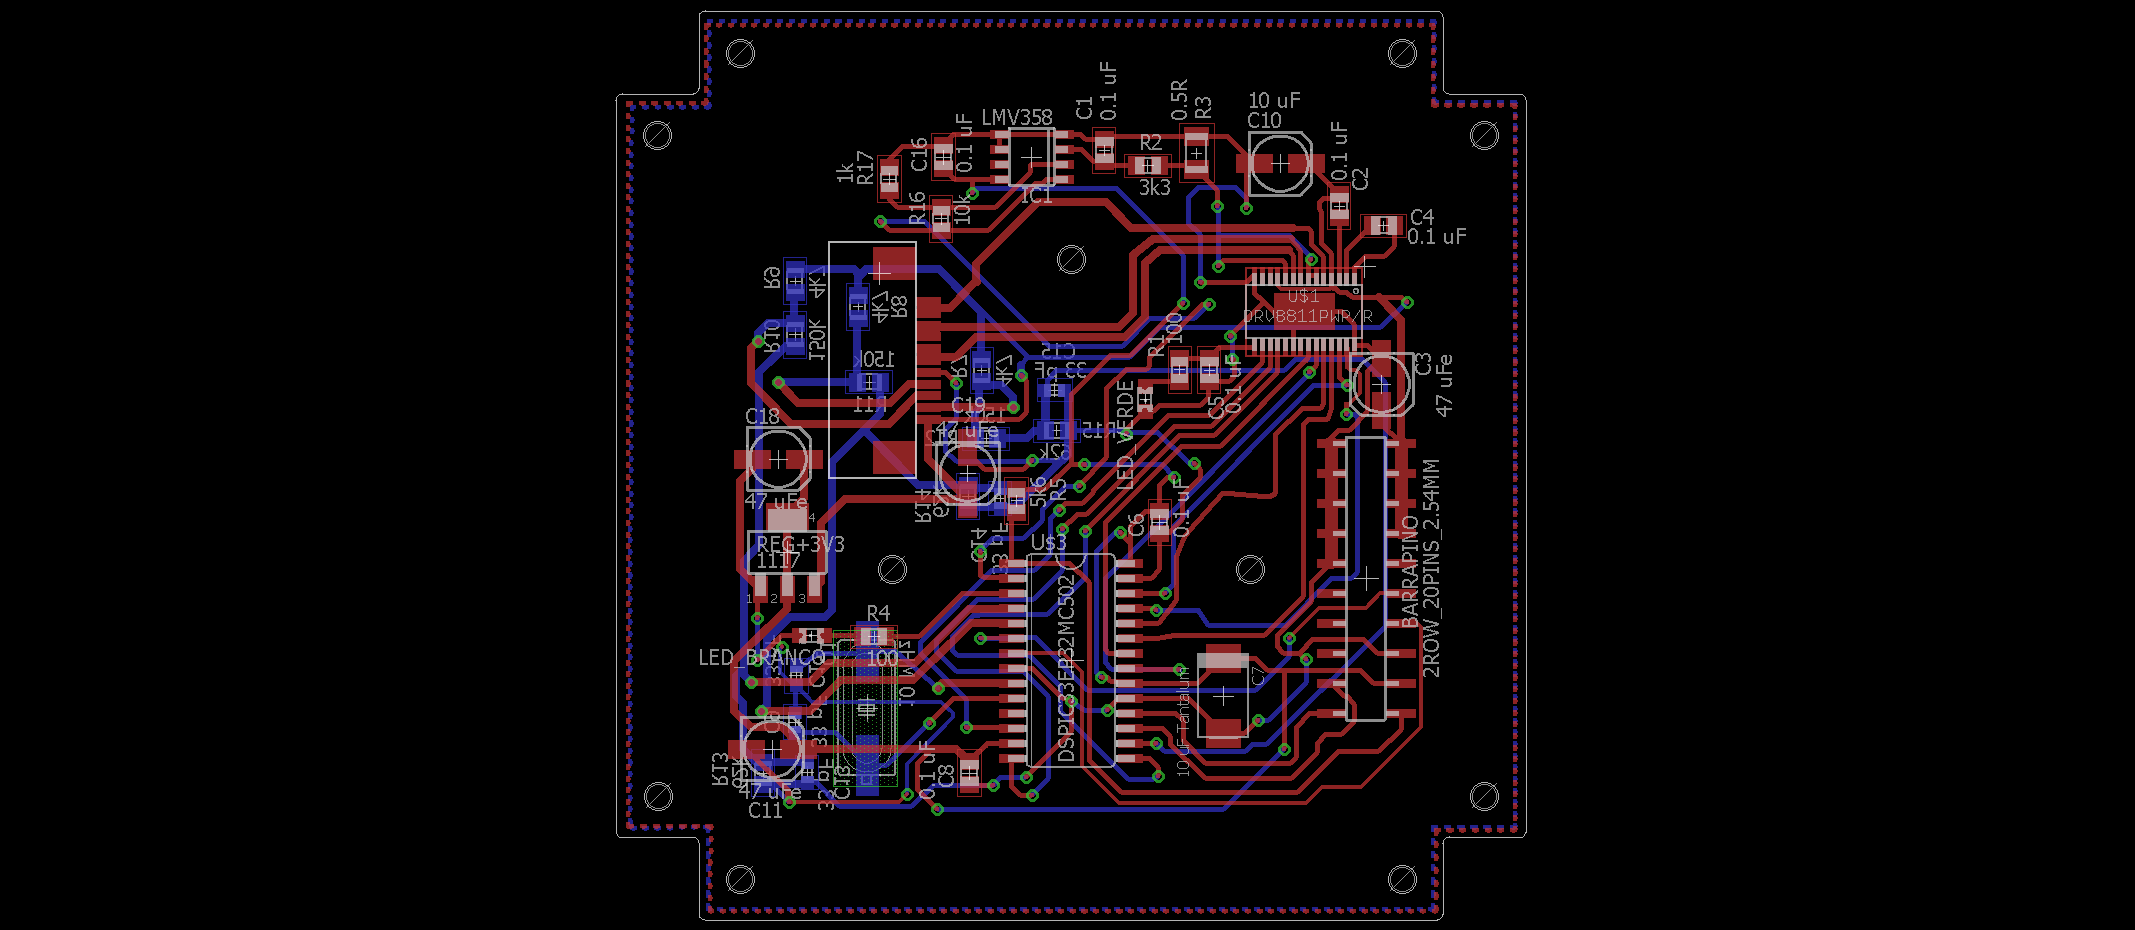
\includegraphics[width=1\linewidth]{./figs/Placa_motores}
\end{figure}

\label{ap:PMotor}

\chapter{Desenho da roda de reação}

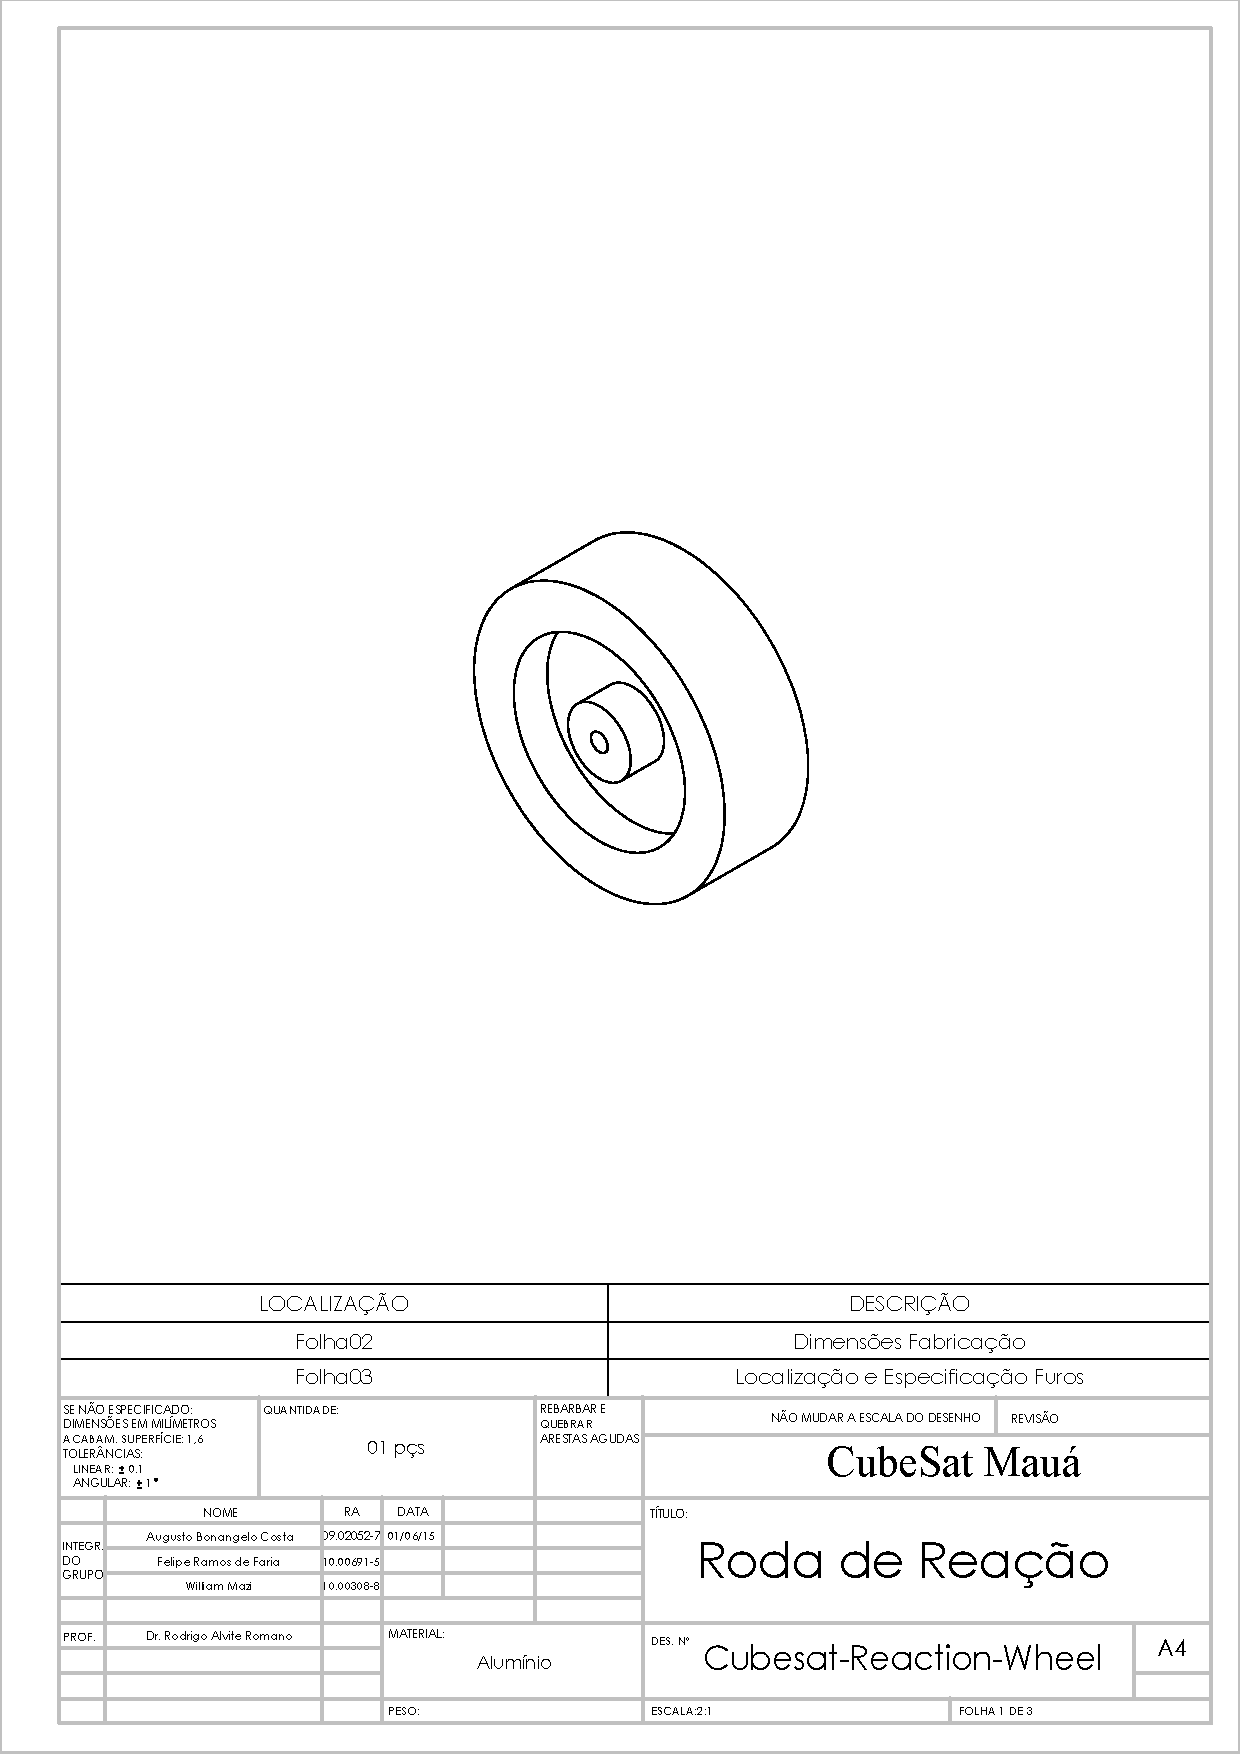
\includepdf[pages=-]{./pdfs/Cubesat-Reaction-Wheel}

\label{ap:RW}

\chapter{Desenho do suporte do motor}

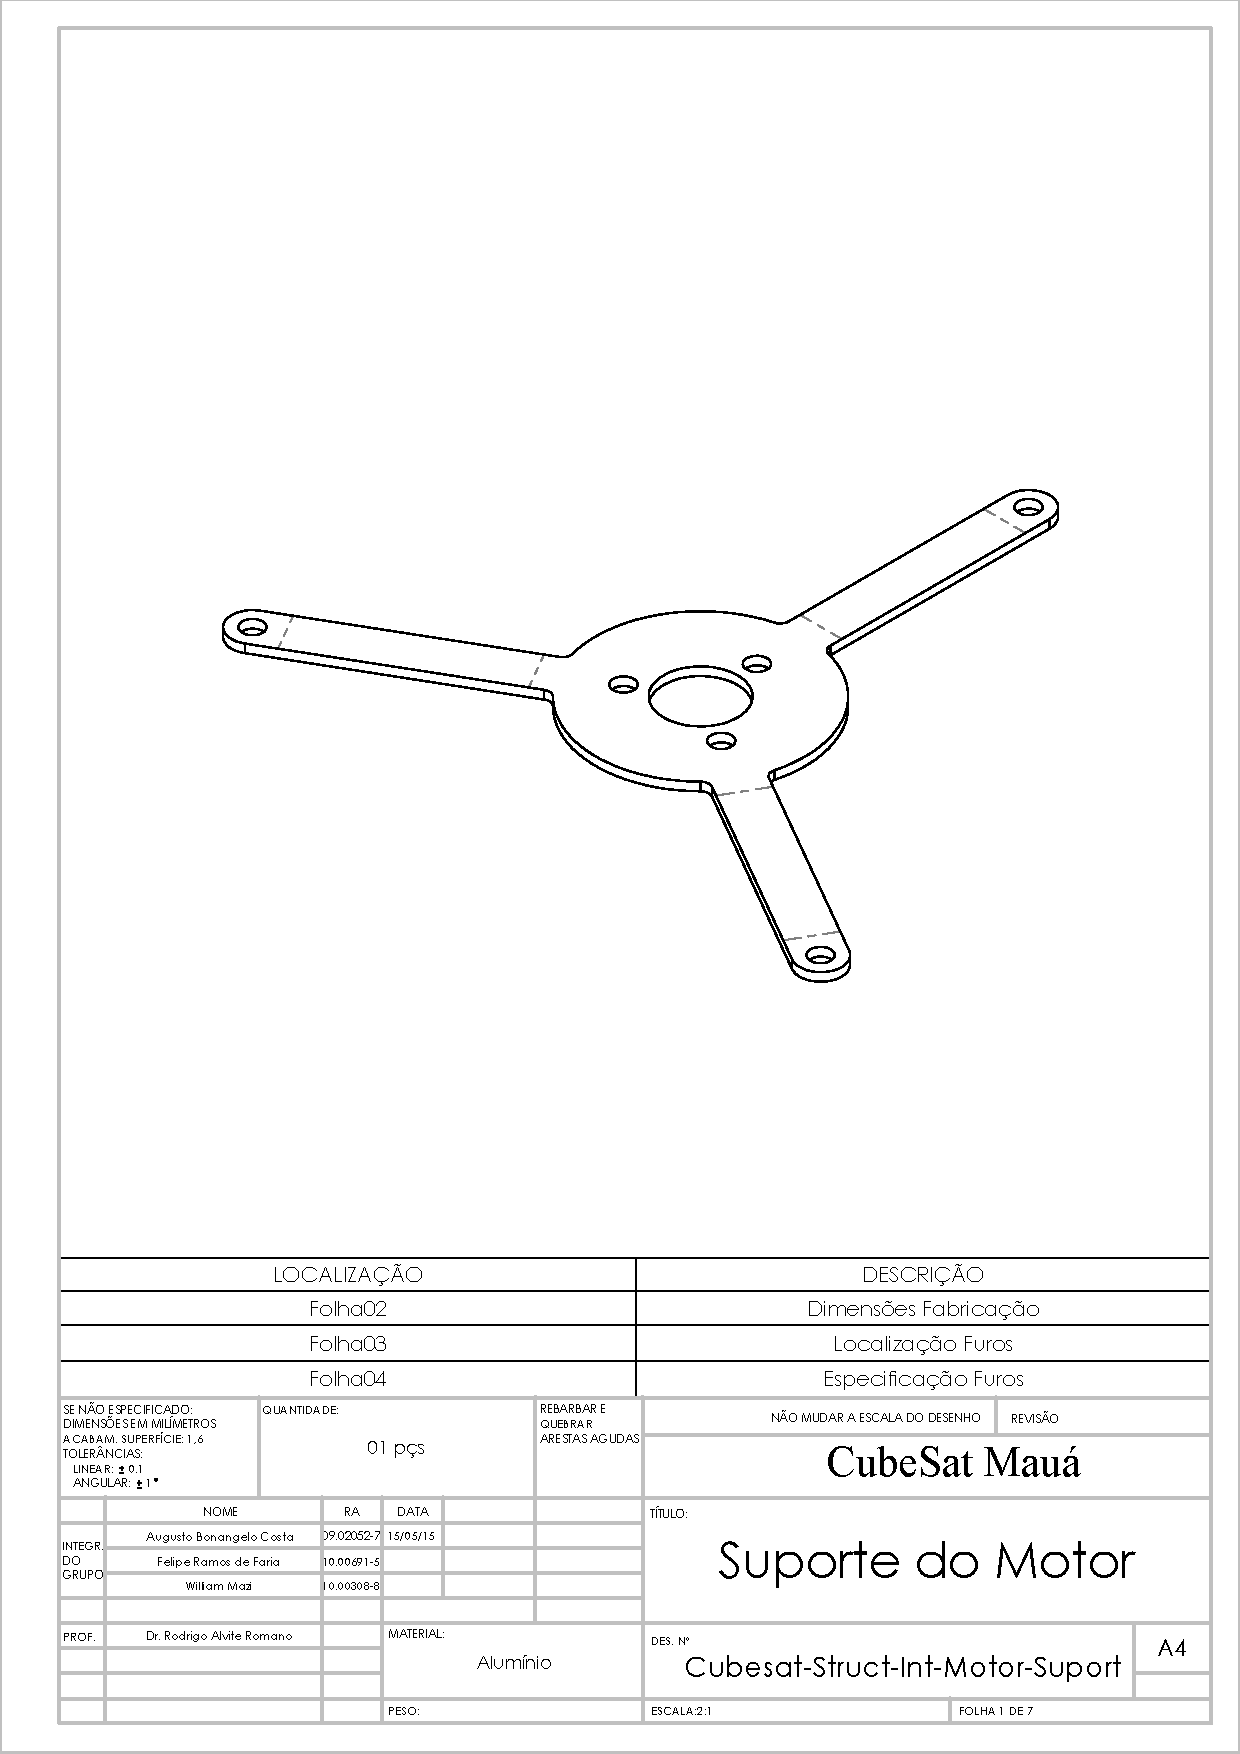
\includepdf[pages=-]{./pdfs/Cubesat-Struct-Int-Motor-Suport}

\label{ap:MS}

\chapter{Desenho da base de testes}

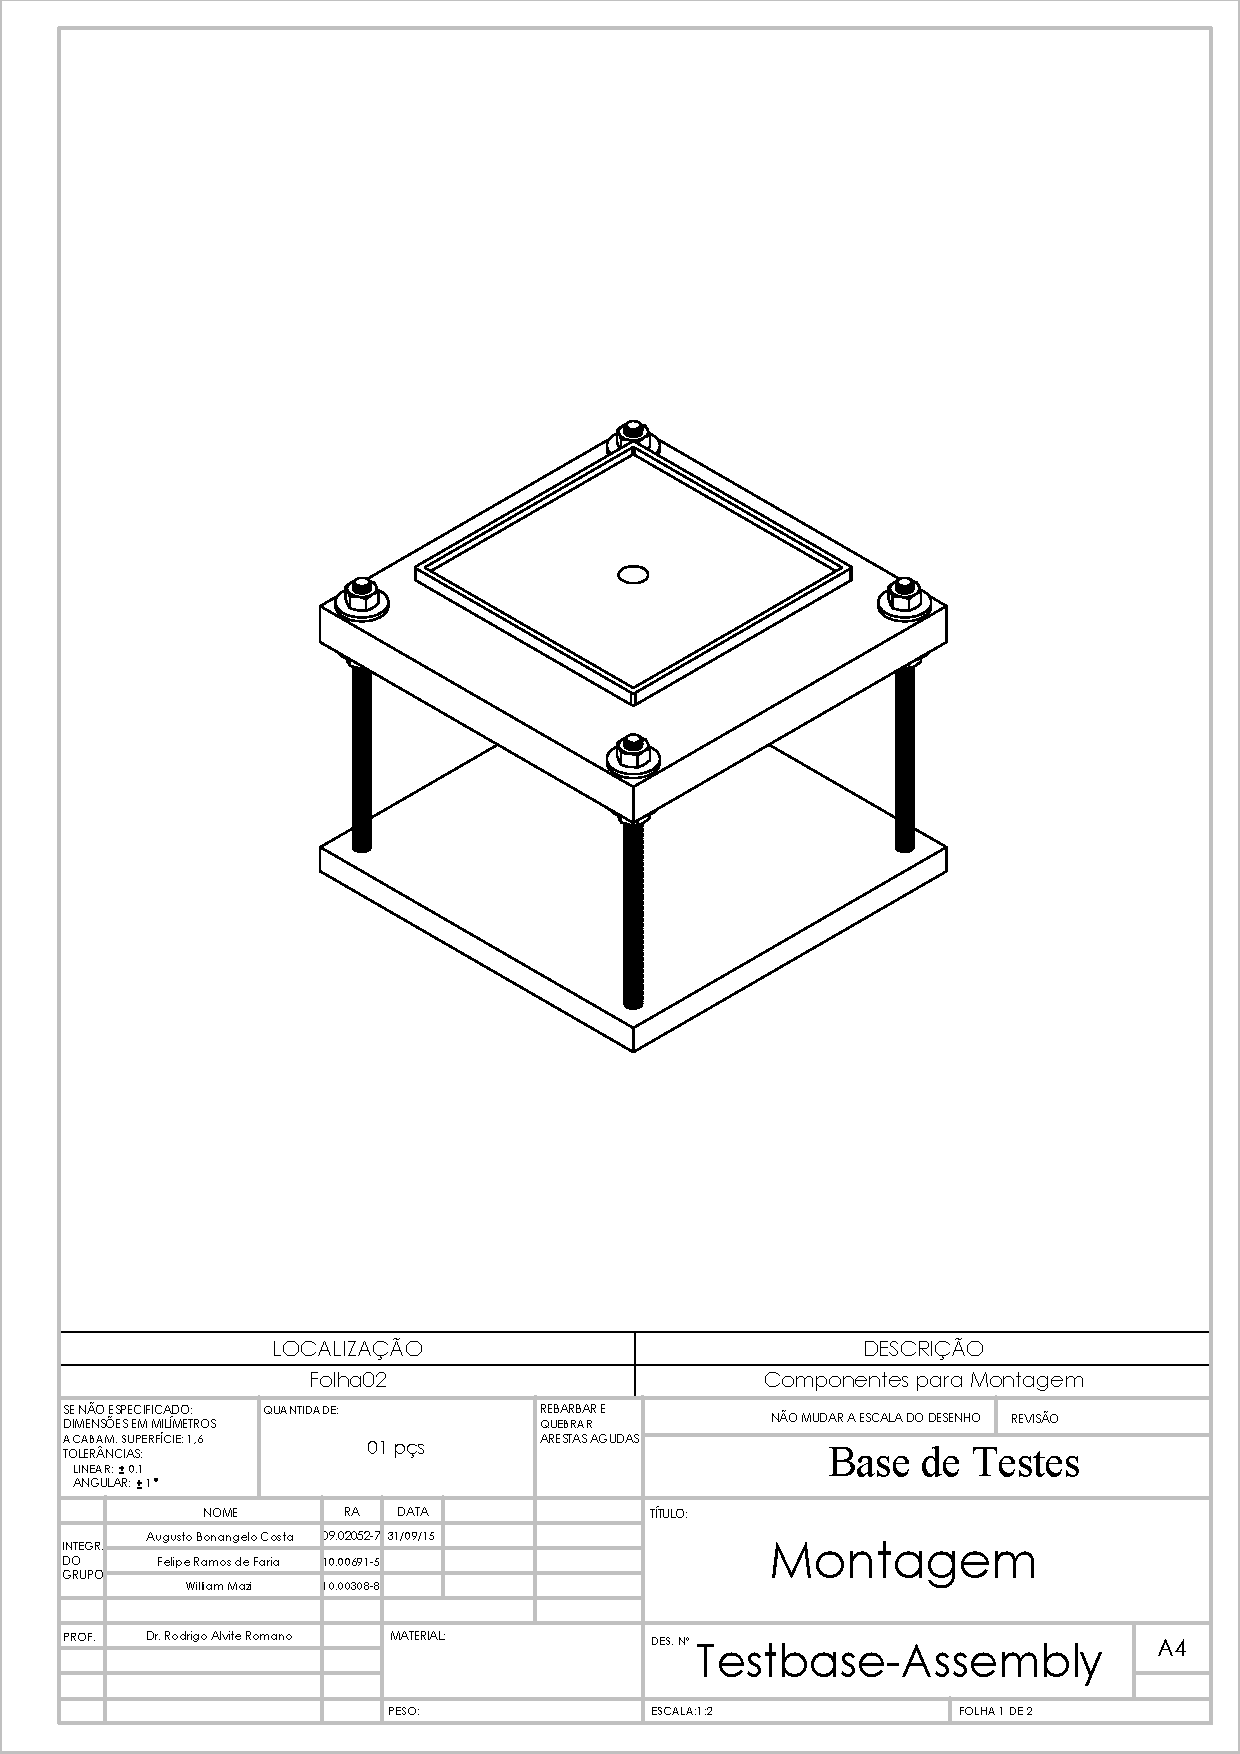
\includepdf[pages=-]{./pdfs/Testbase-Assembly}
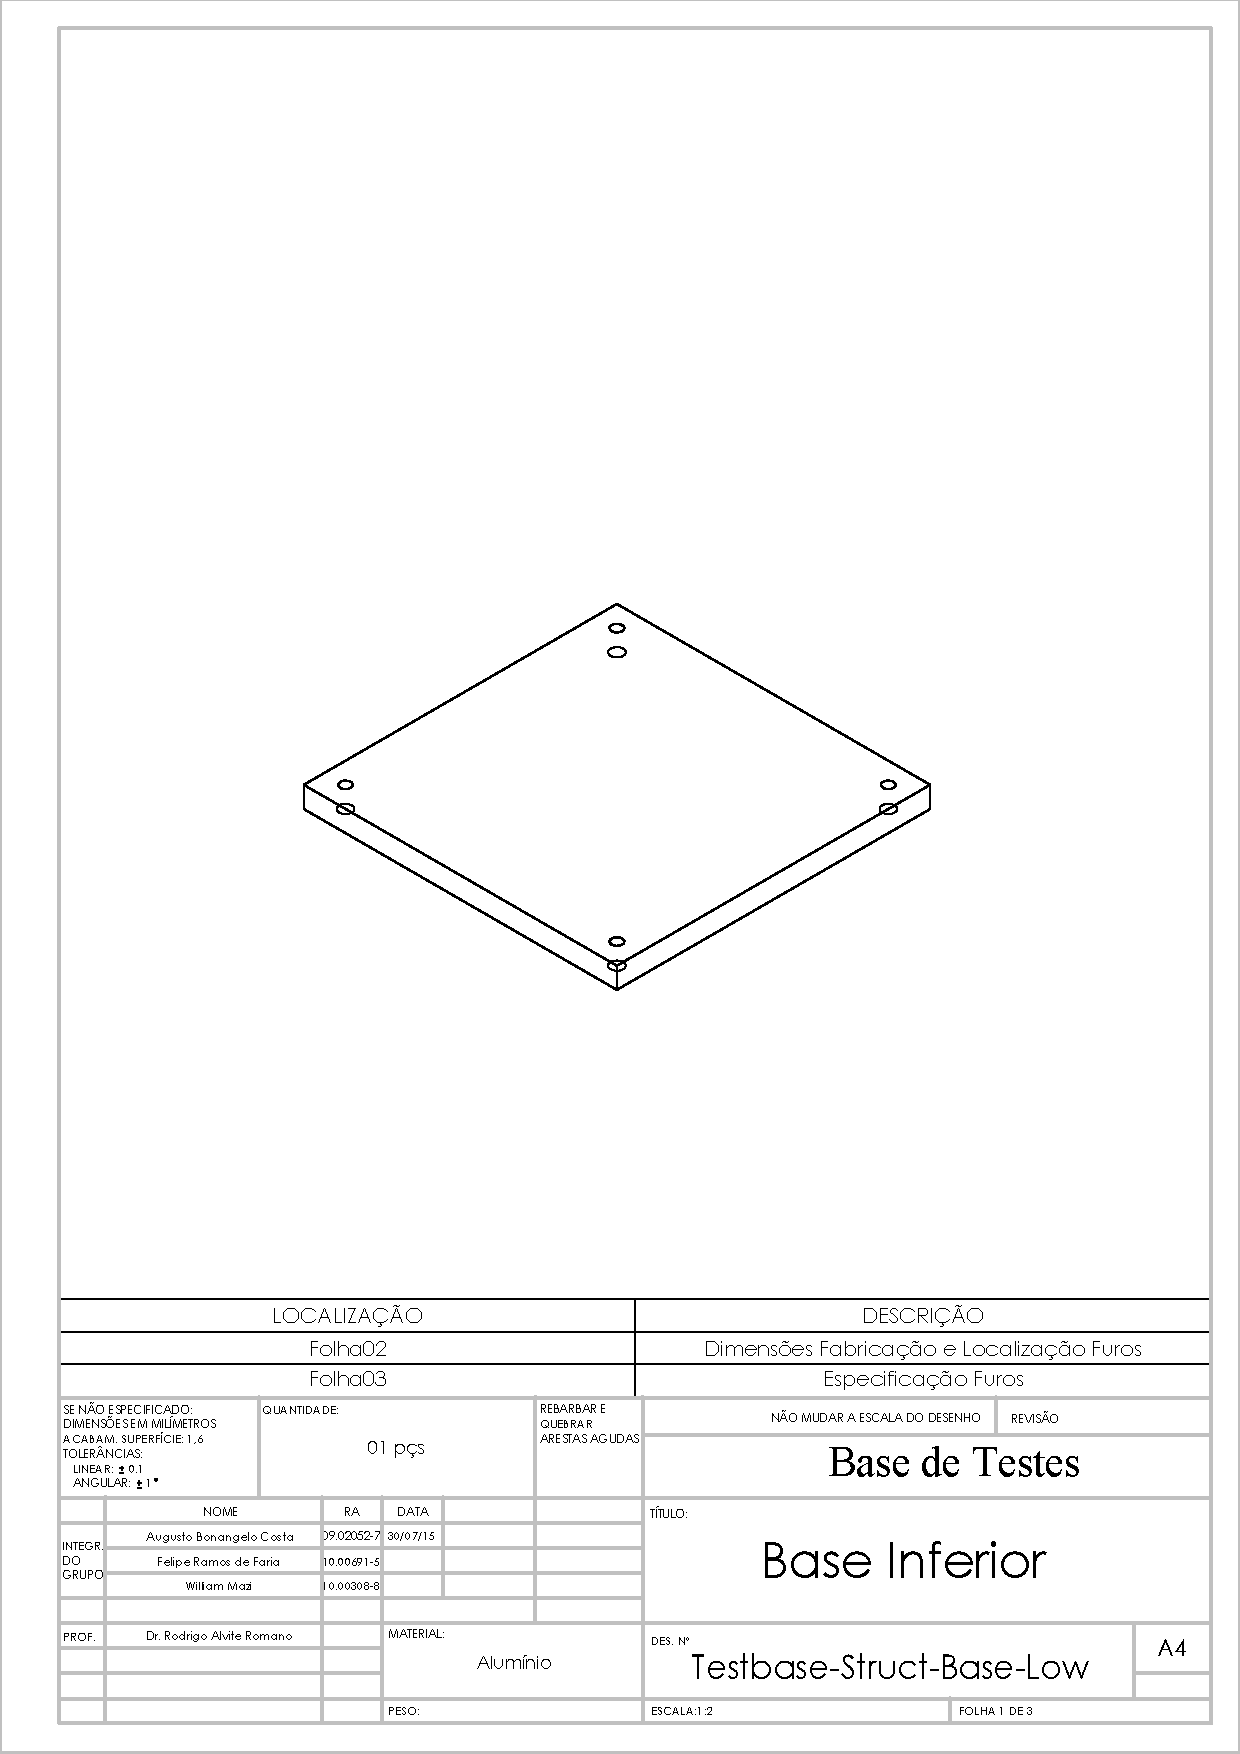
\includepdf[pages=-]{./pdfs/Testbase-Struct-Base-Low}
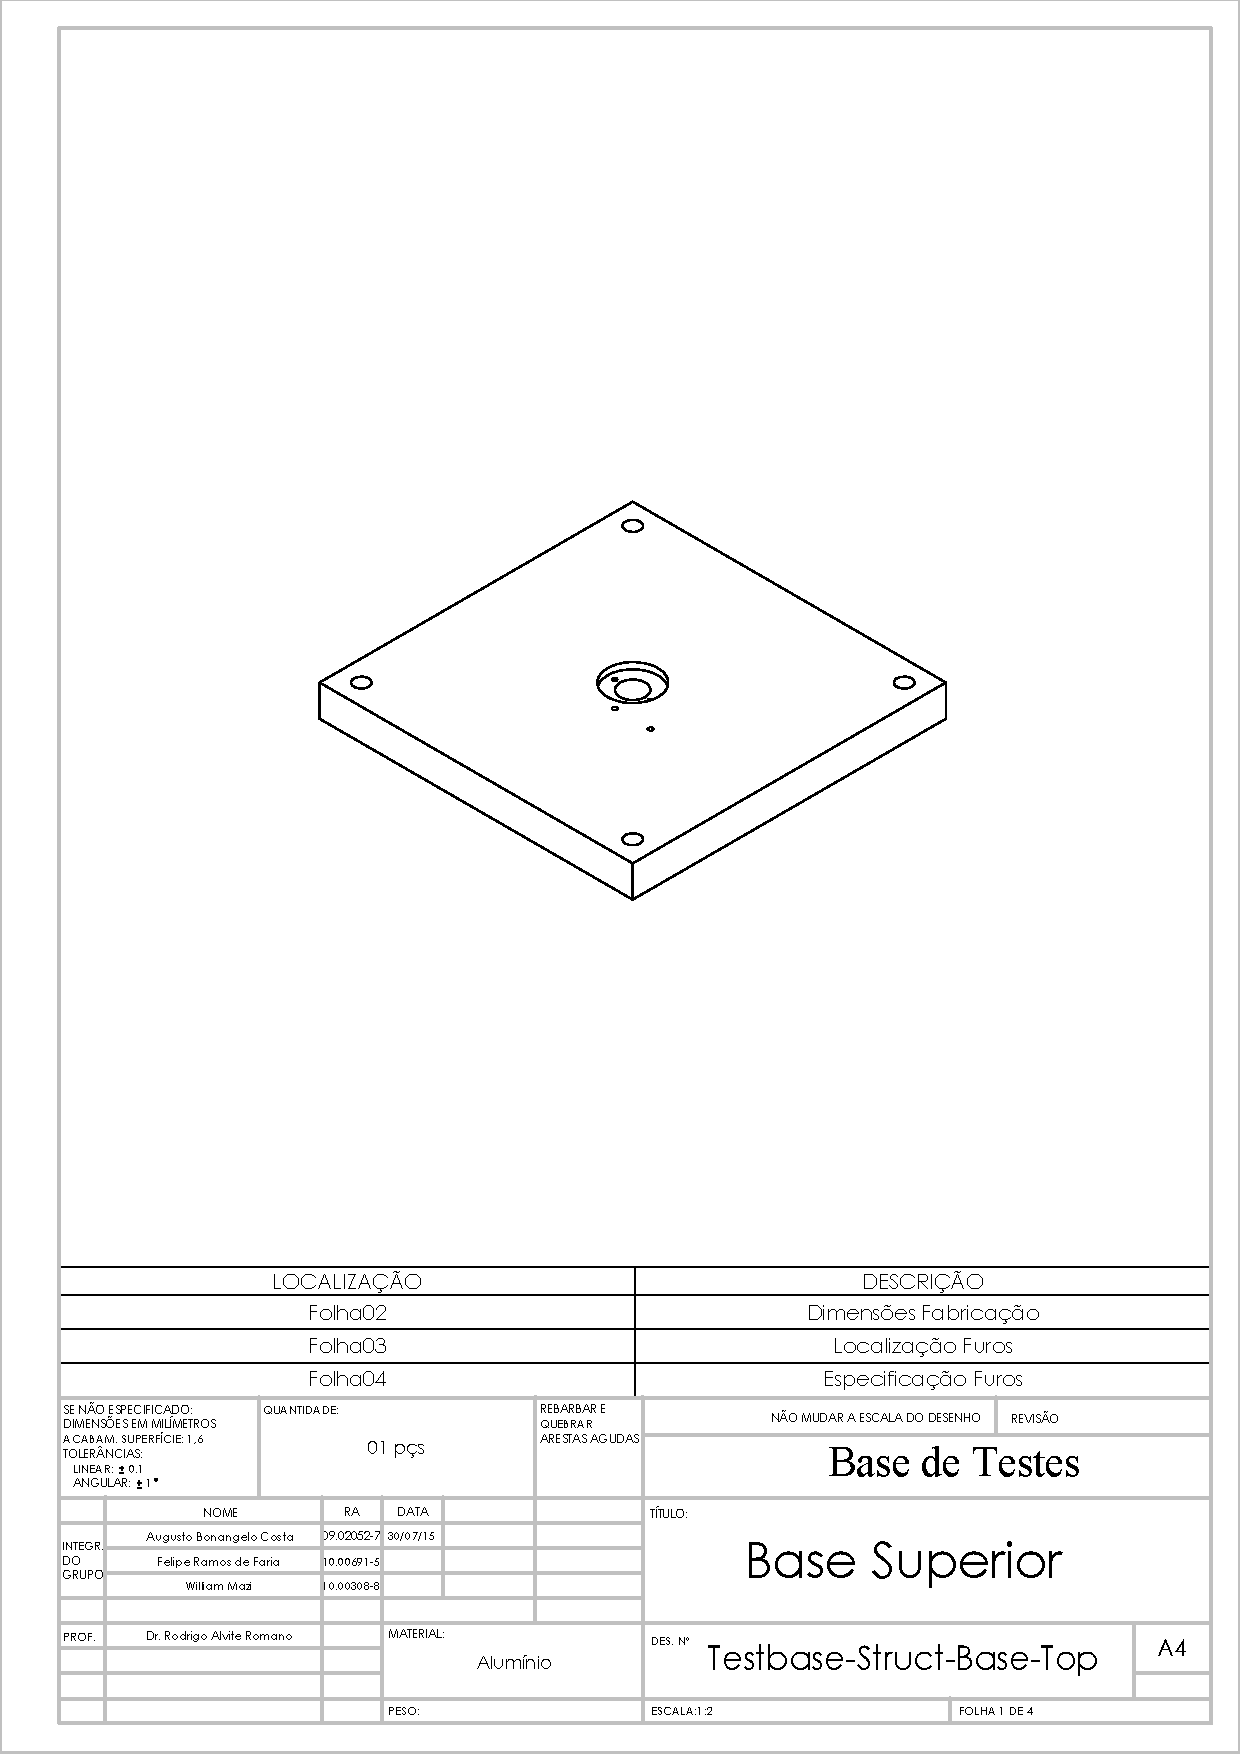
\includepdf[pages=-]{./pdfs/Testbase-Struct-Base-Top}
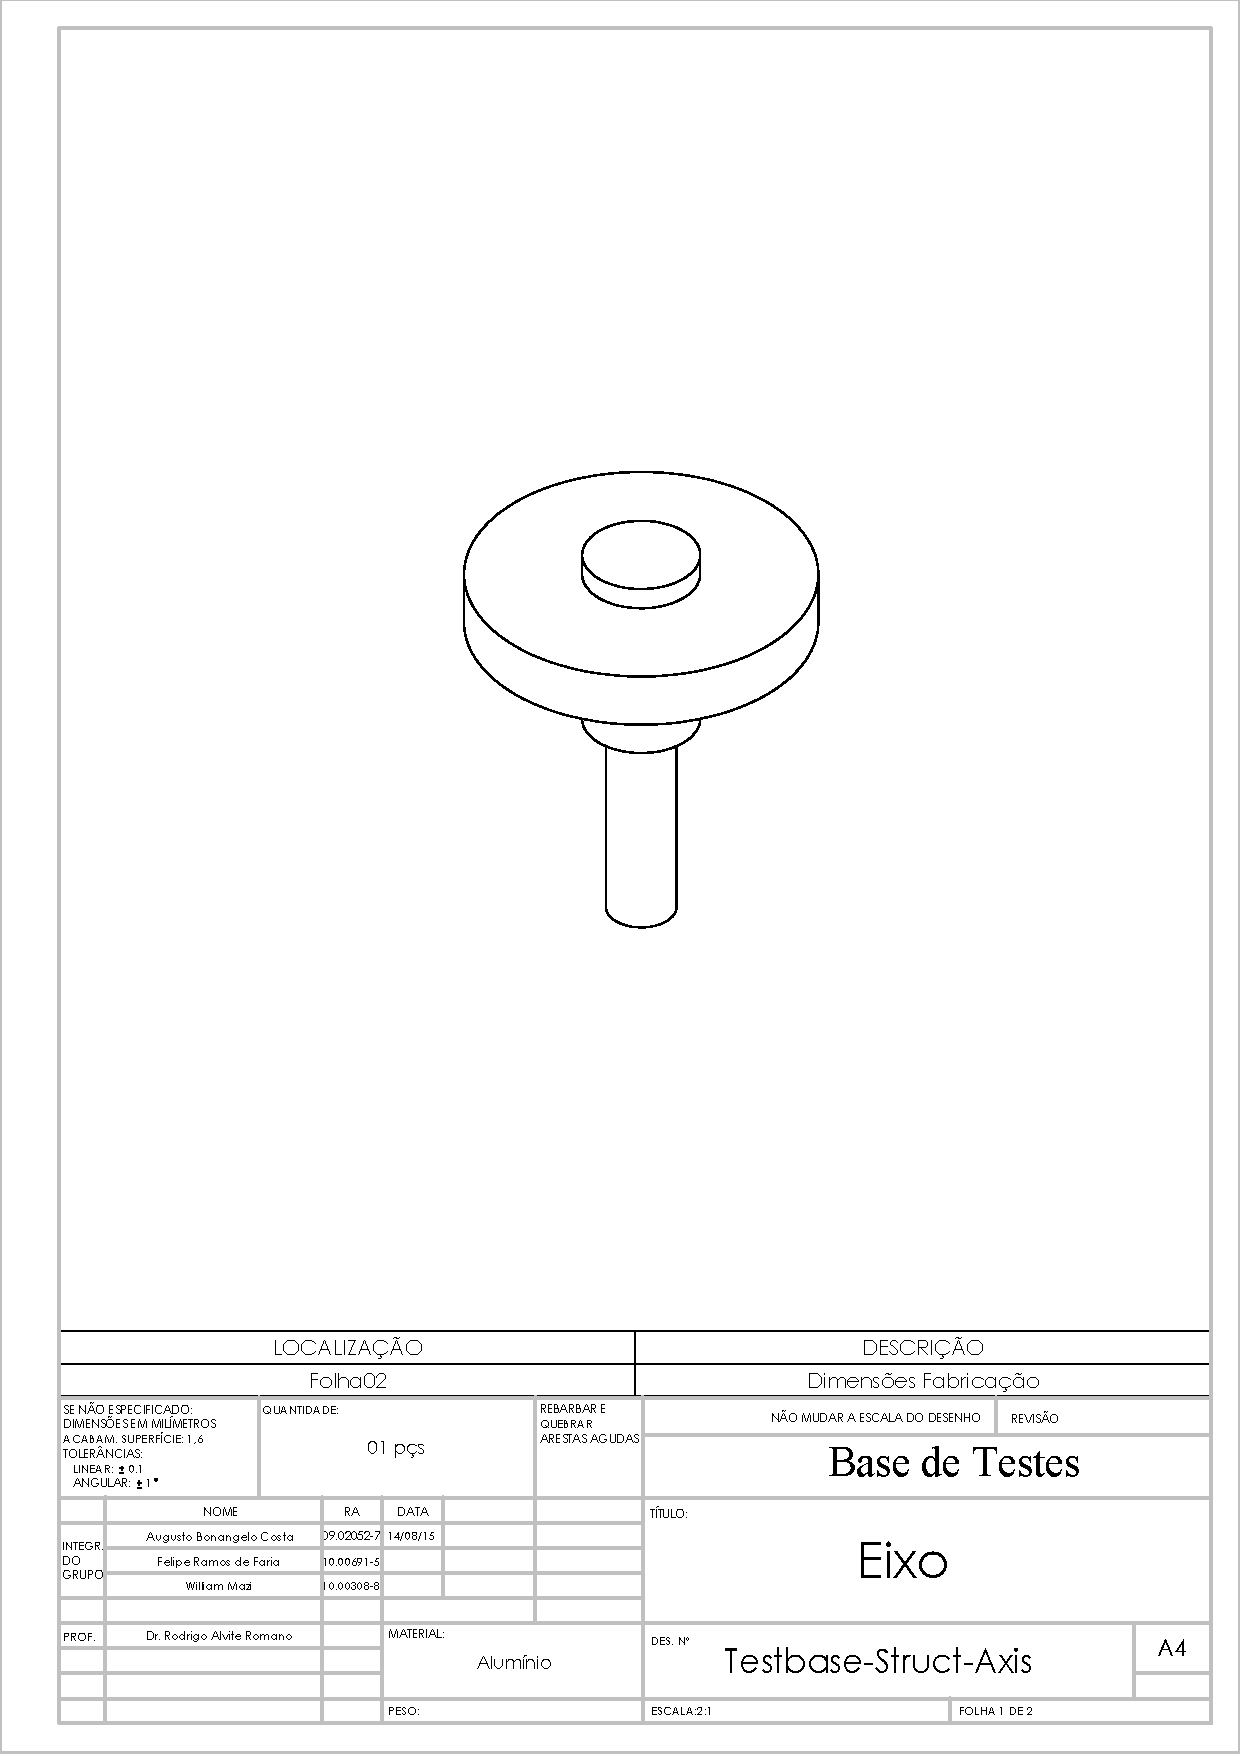
\includepdf[pages=-]{./pdfs/Testbase-Struct-Axis}
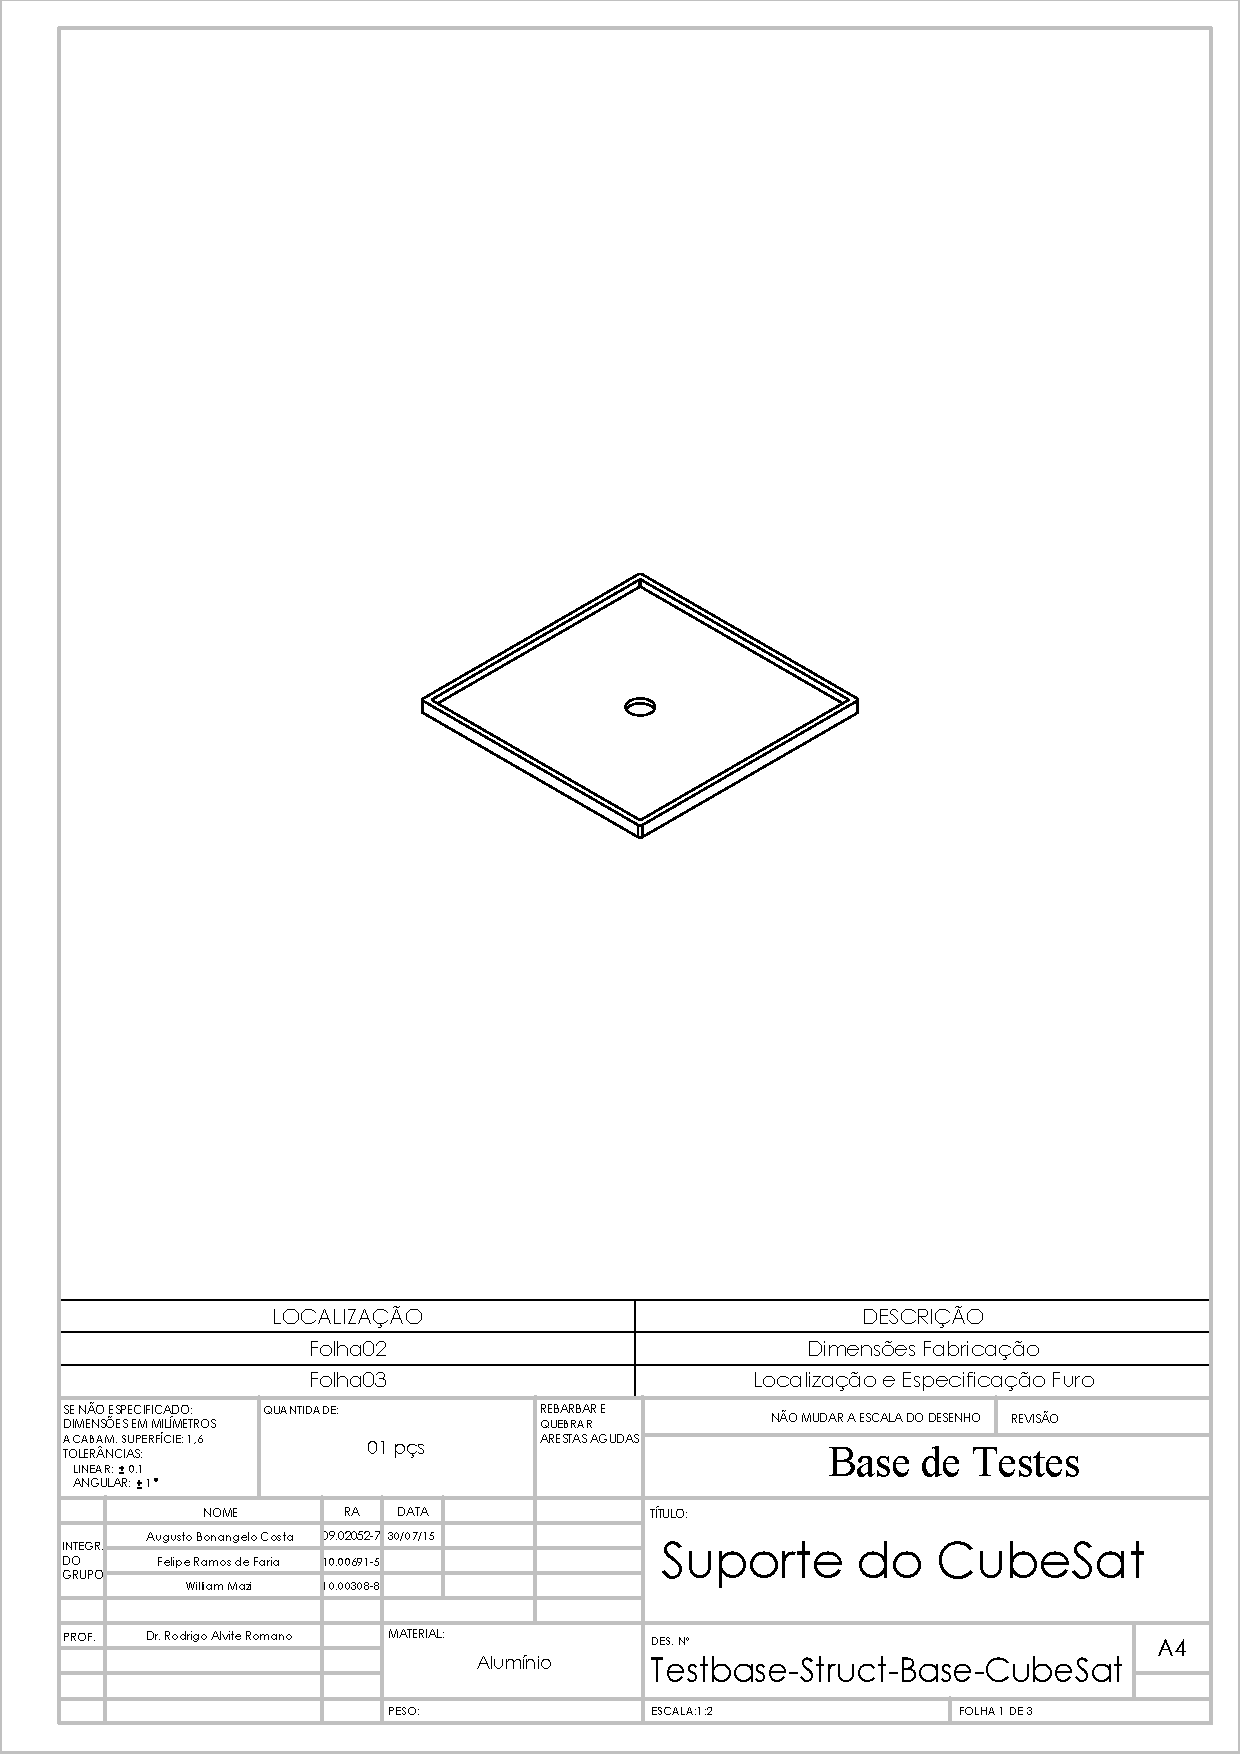
\includepdf[pages=-]{./pdfs/Testbase-Struct-Base-CubeSat}

\label{ap:TB}

\end{apendicesenv}

% ----------------------------------------------------------
% Anexos
% ----------------------------------------------------------
% Inicia os anexos
% ---
\begin{anexosenv}
% Imprime uma página indicando o início dos anexos
\partanexos
% ---
\chapter{Página do catálogo do motor \textit{brushless} 351100 da Maxon}

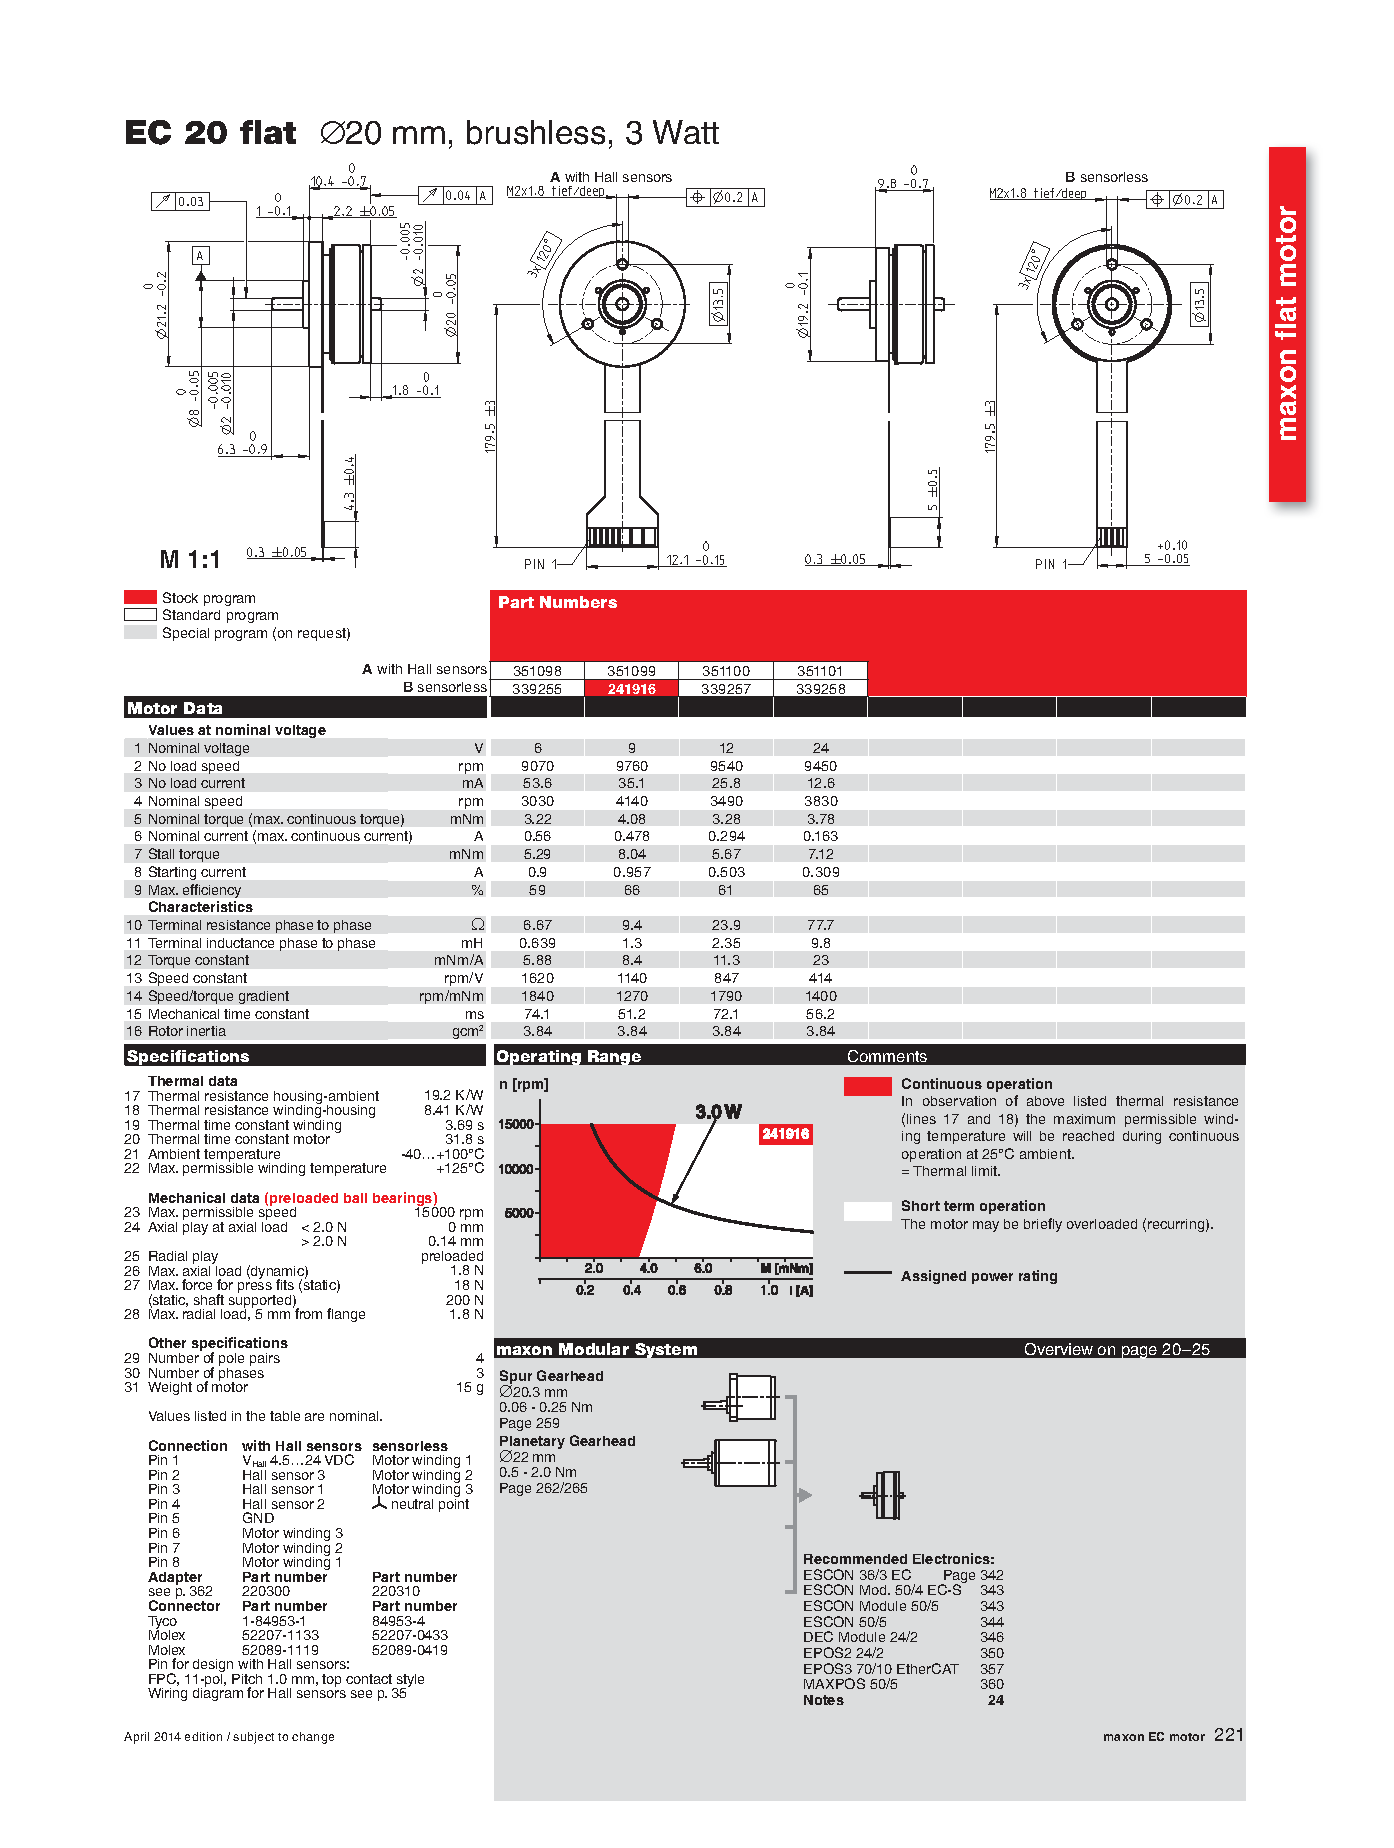
\includepdf[pages=-]{./pdfs/351100}

\label{an:MM}

%\chapter{Desenho da estrutura mecânica do CubeSat}

%\label{an:MS}

%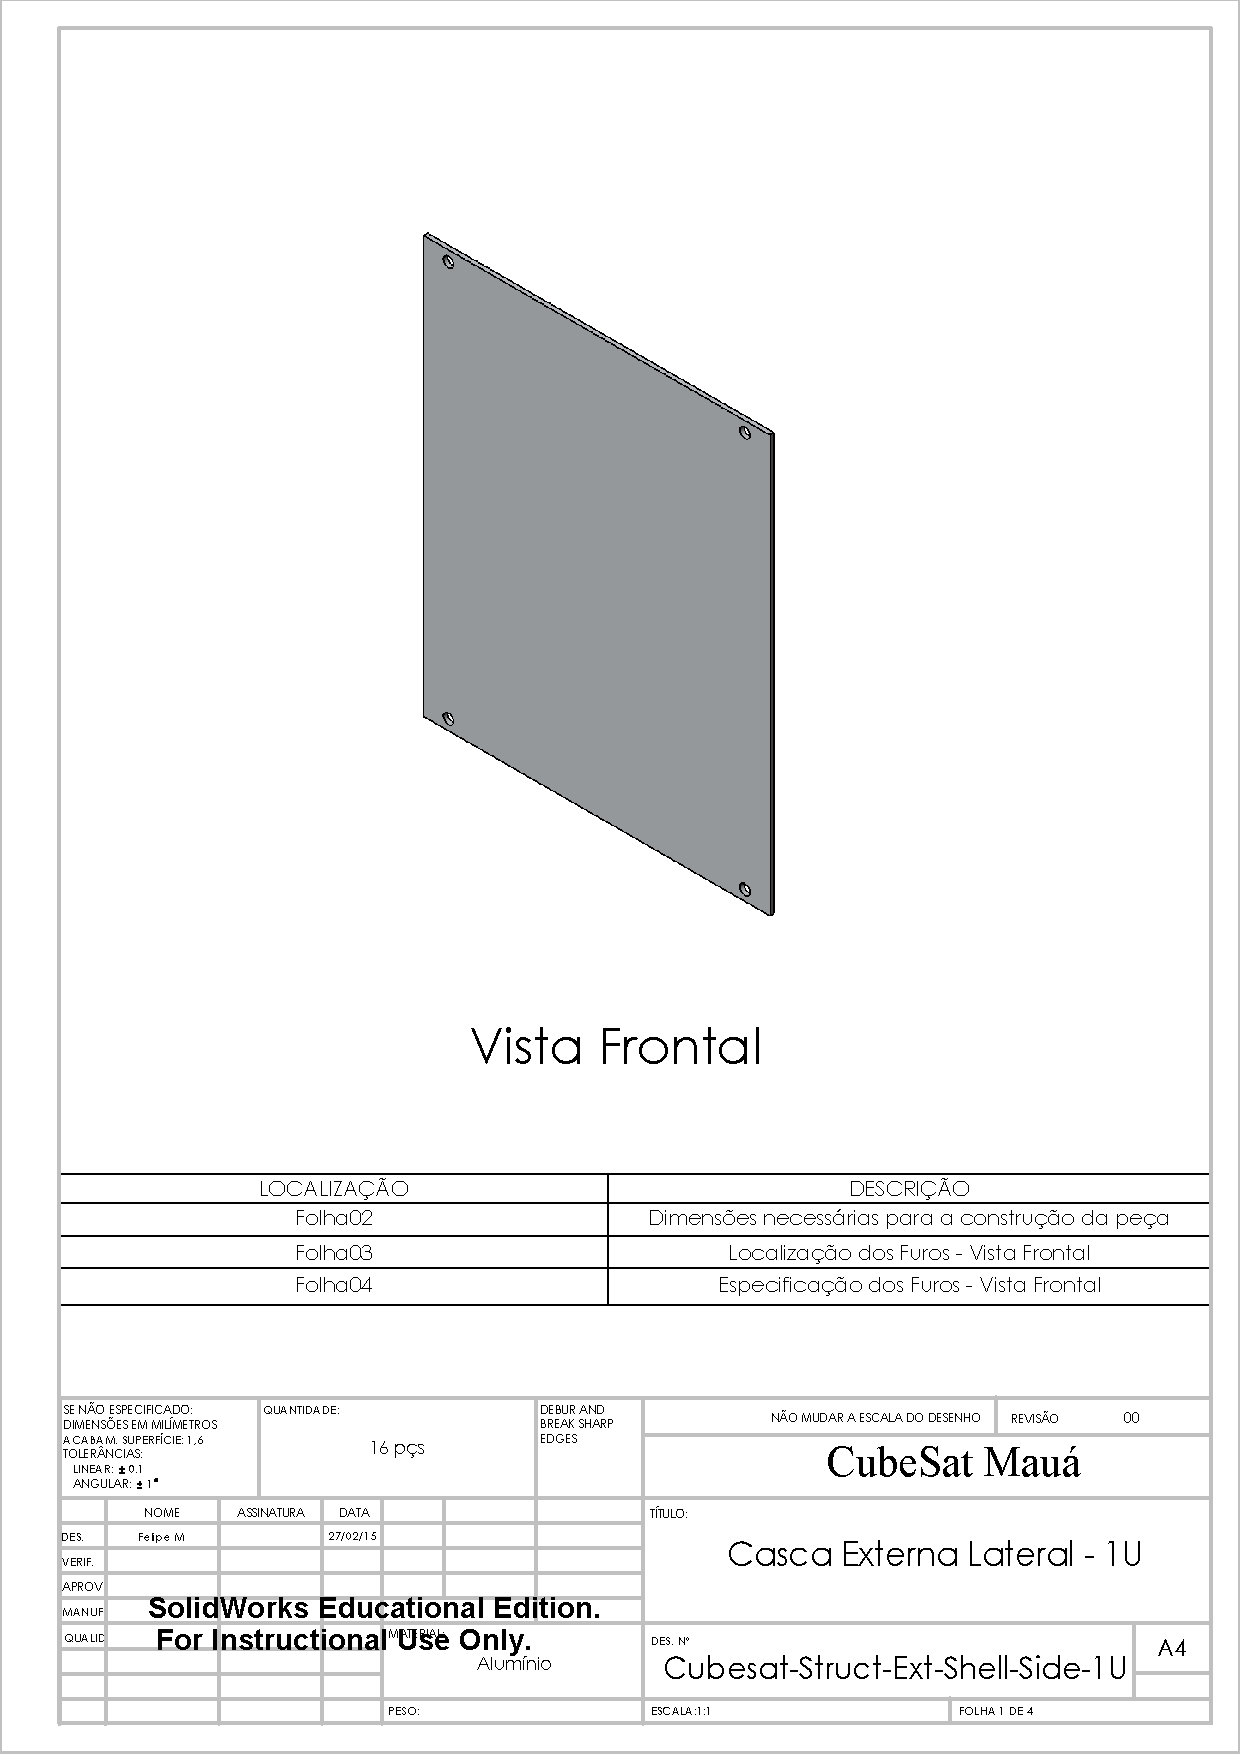
\includepdf[pages=-]{./pdfs/Cubesat-Struct-Ext-Shell-Side-1U}
%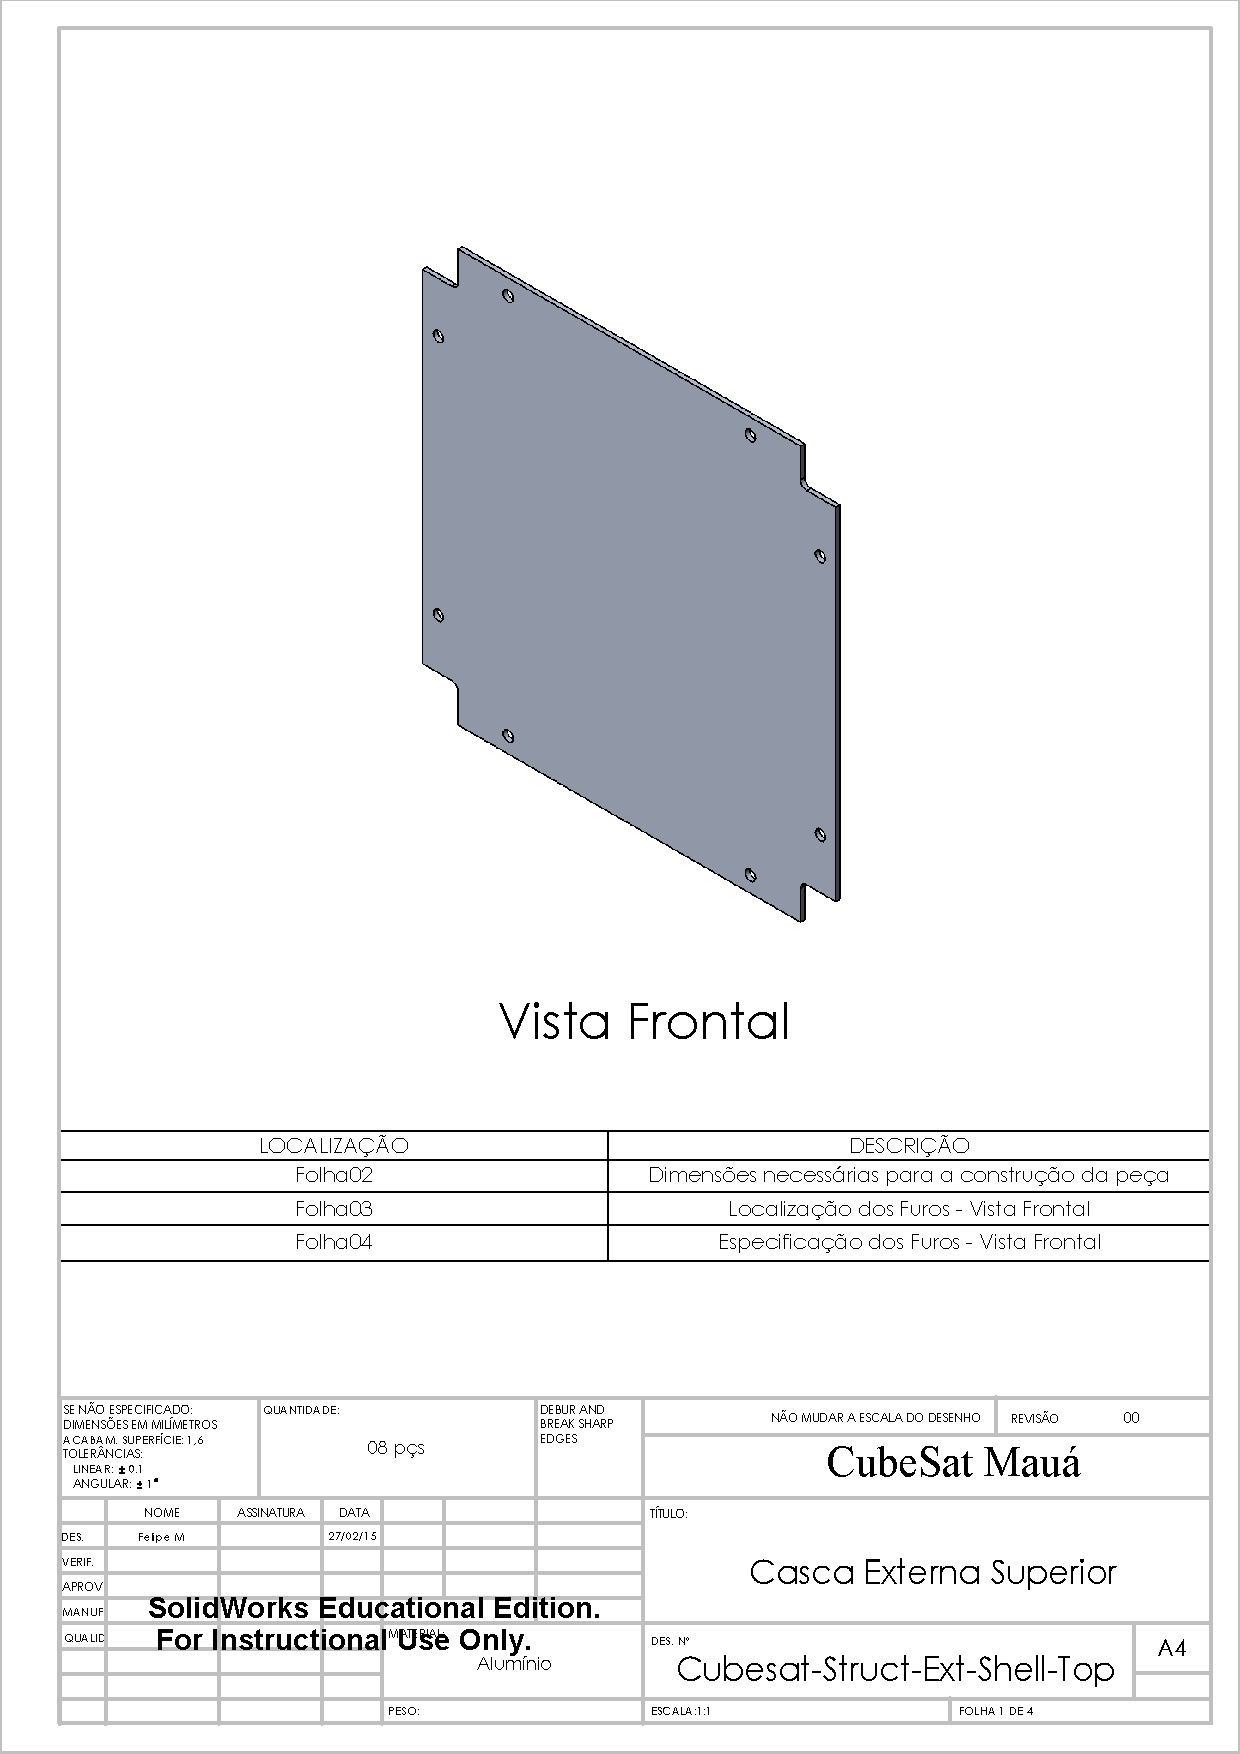
\includepdf[pages=-]{./pdfs/Cubesat-Struct-Ext-Shell-Top}
%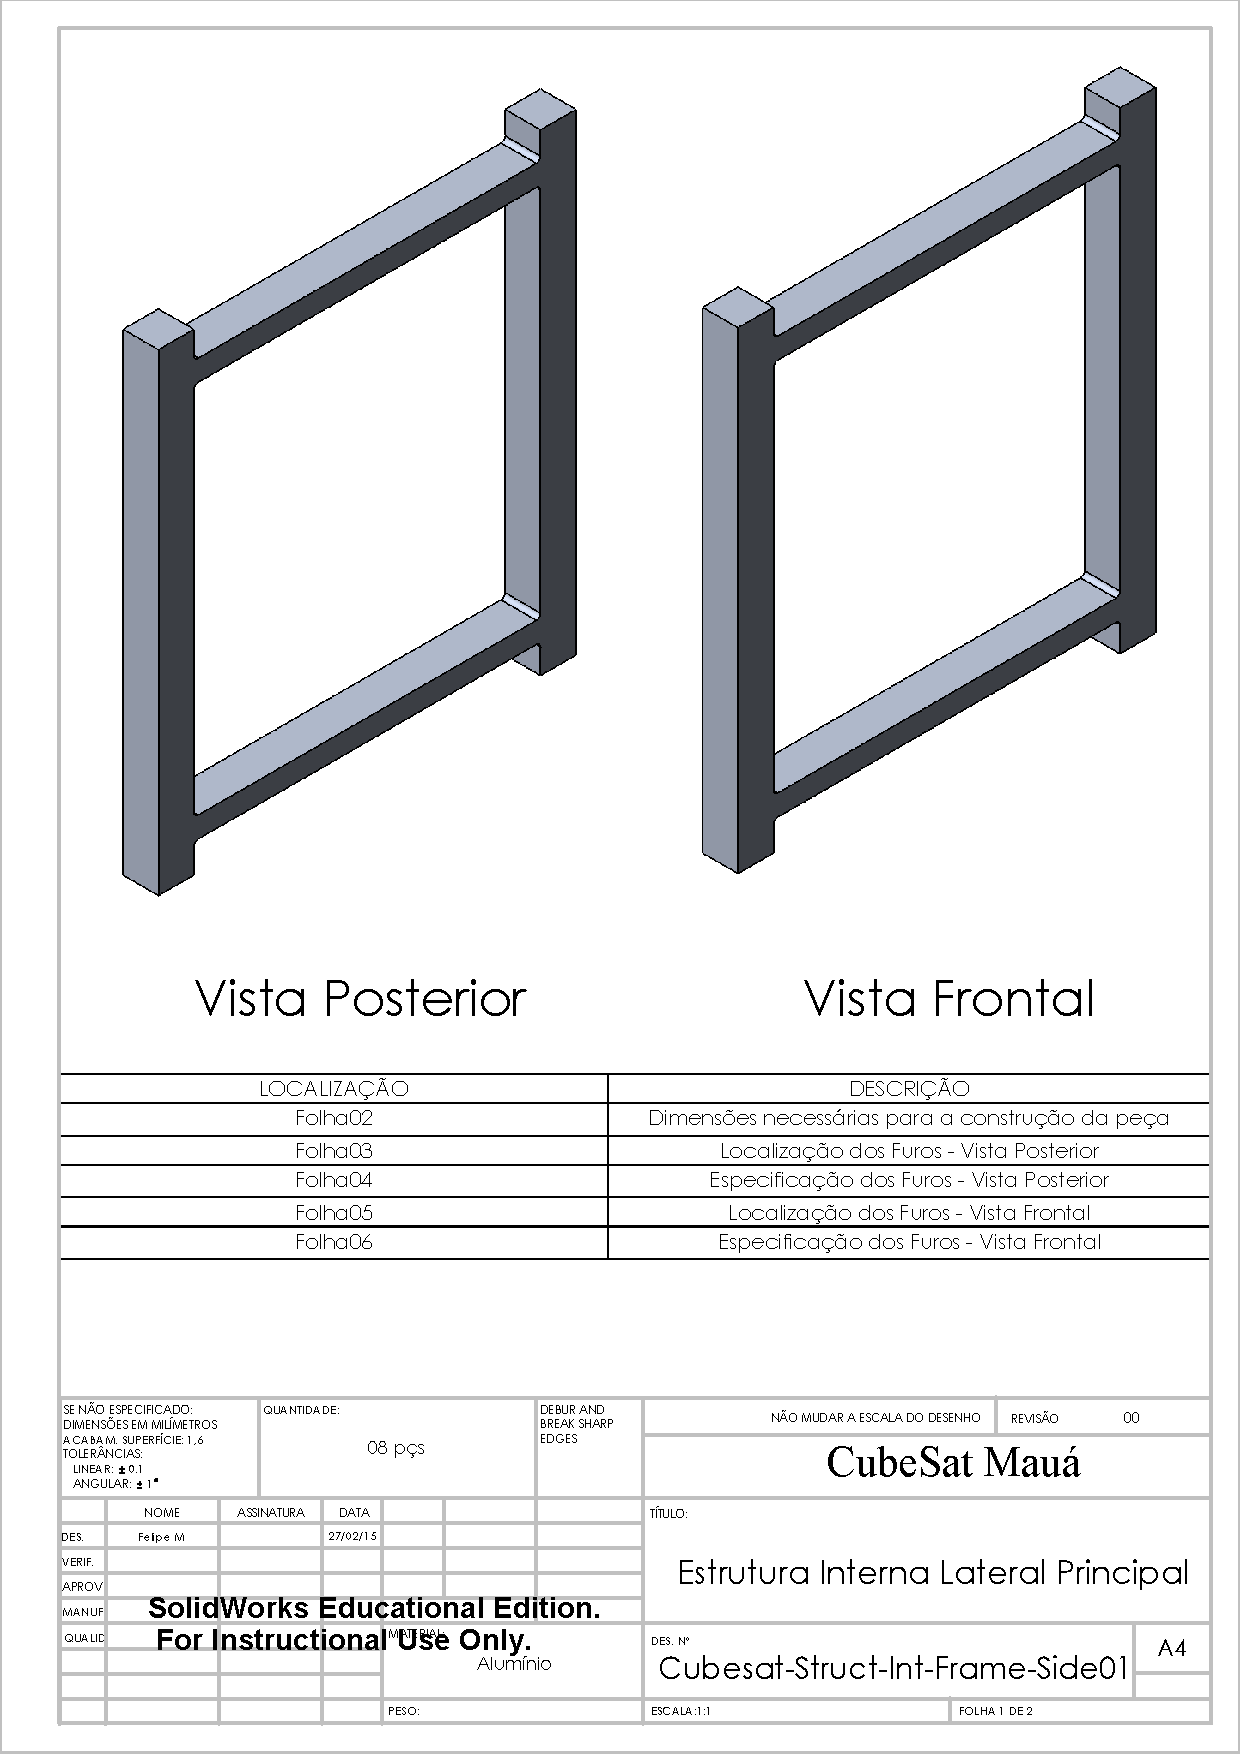
\includepdf[pages=-]{./pdfs/Cubesat-Struct-Int-Frame-Side01}
%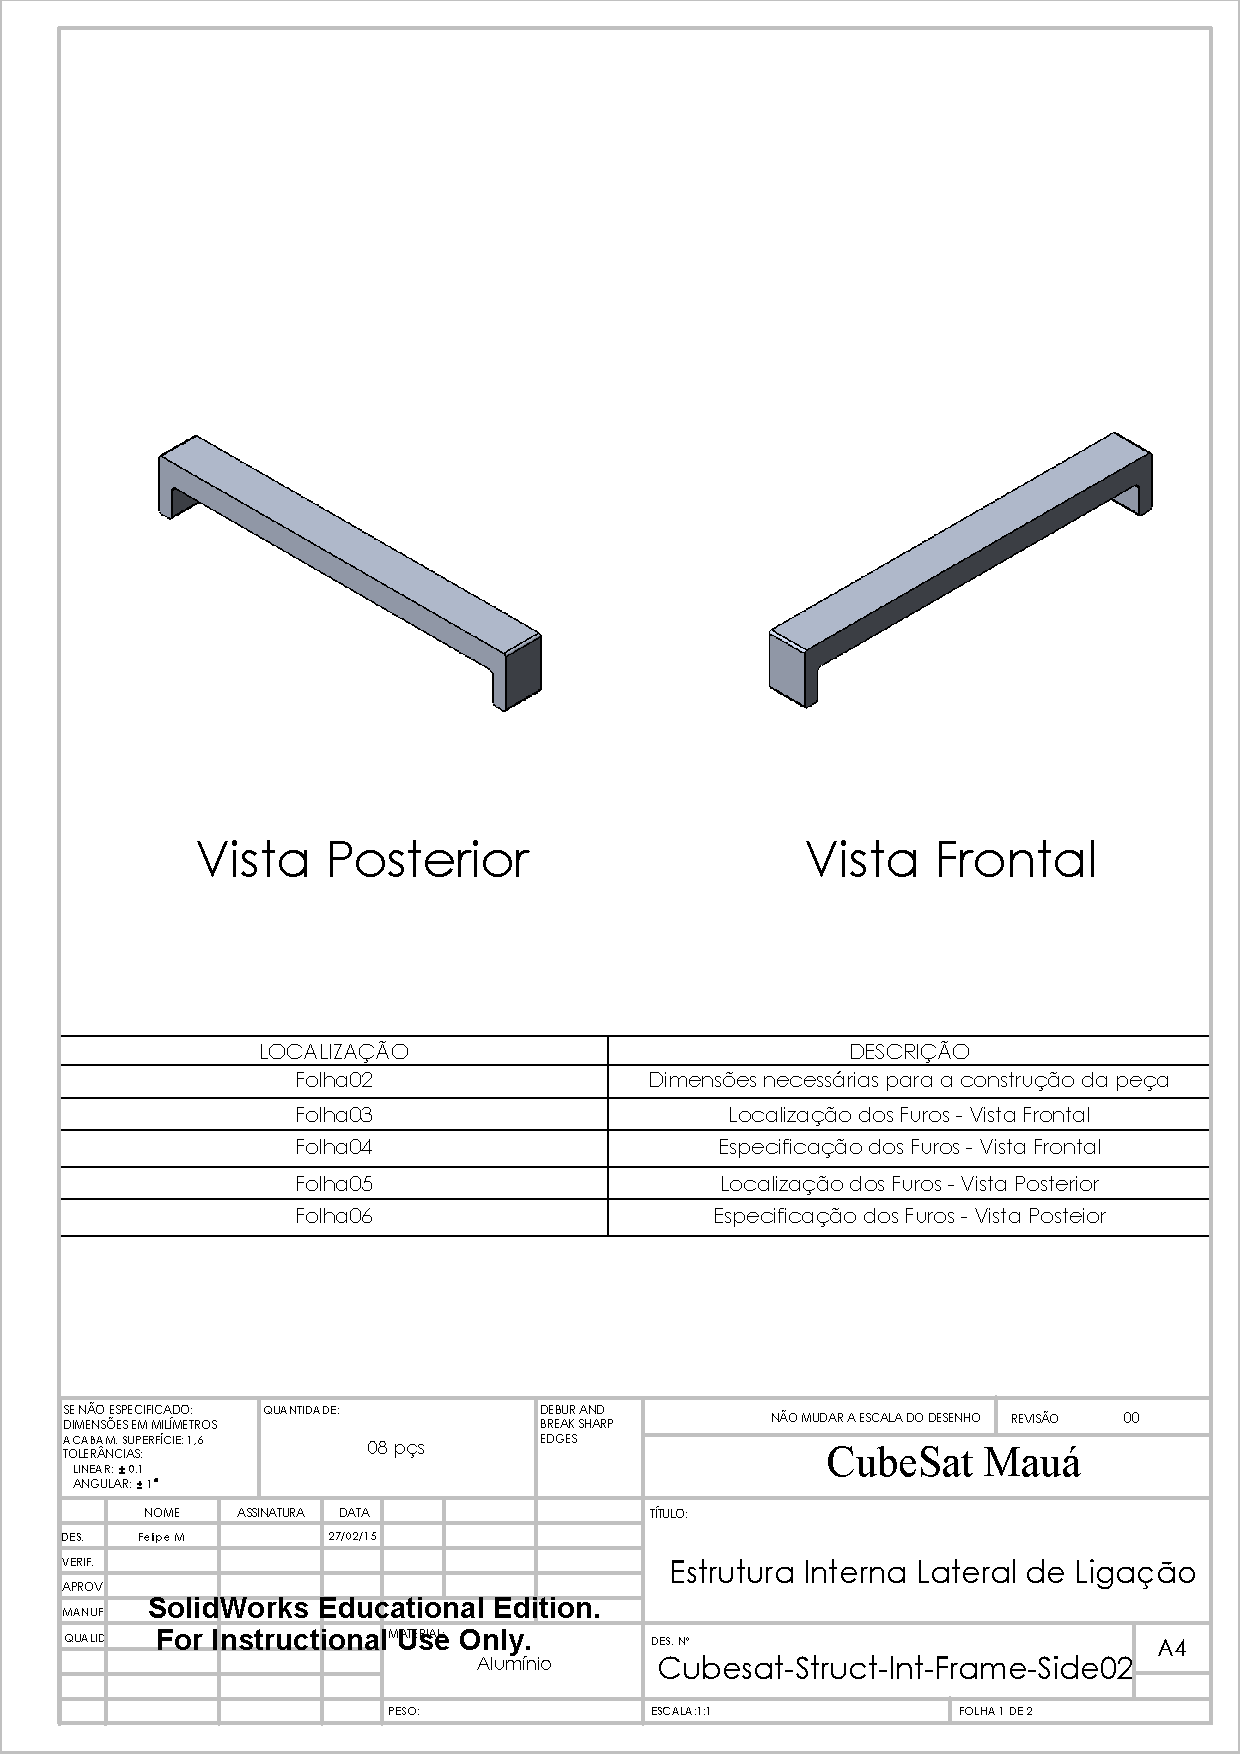
\includepdf[pages=-]{./pdfs/Cubesat-Struct-Int-Frame-Side02}
%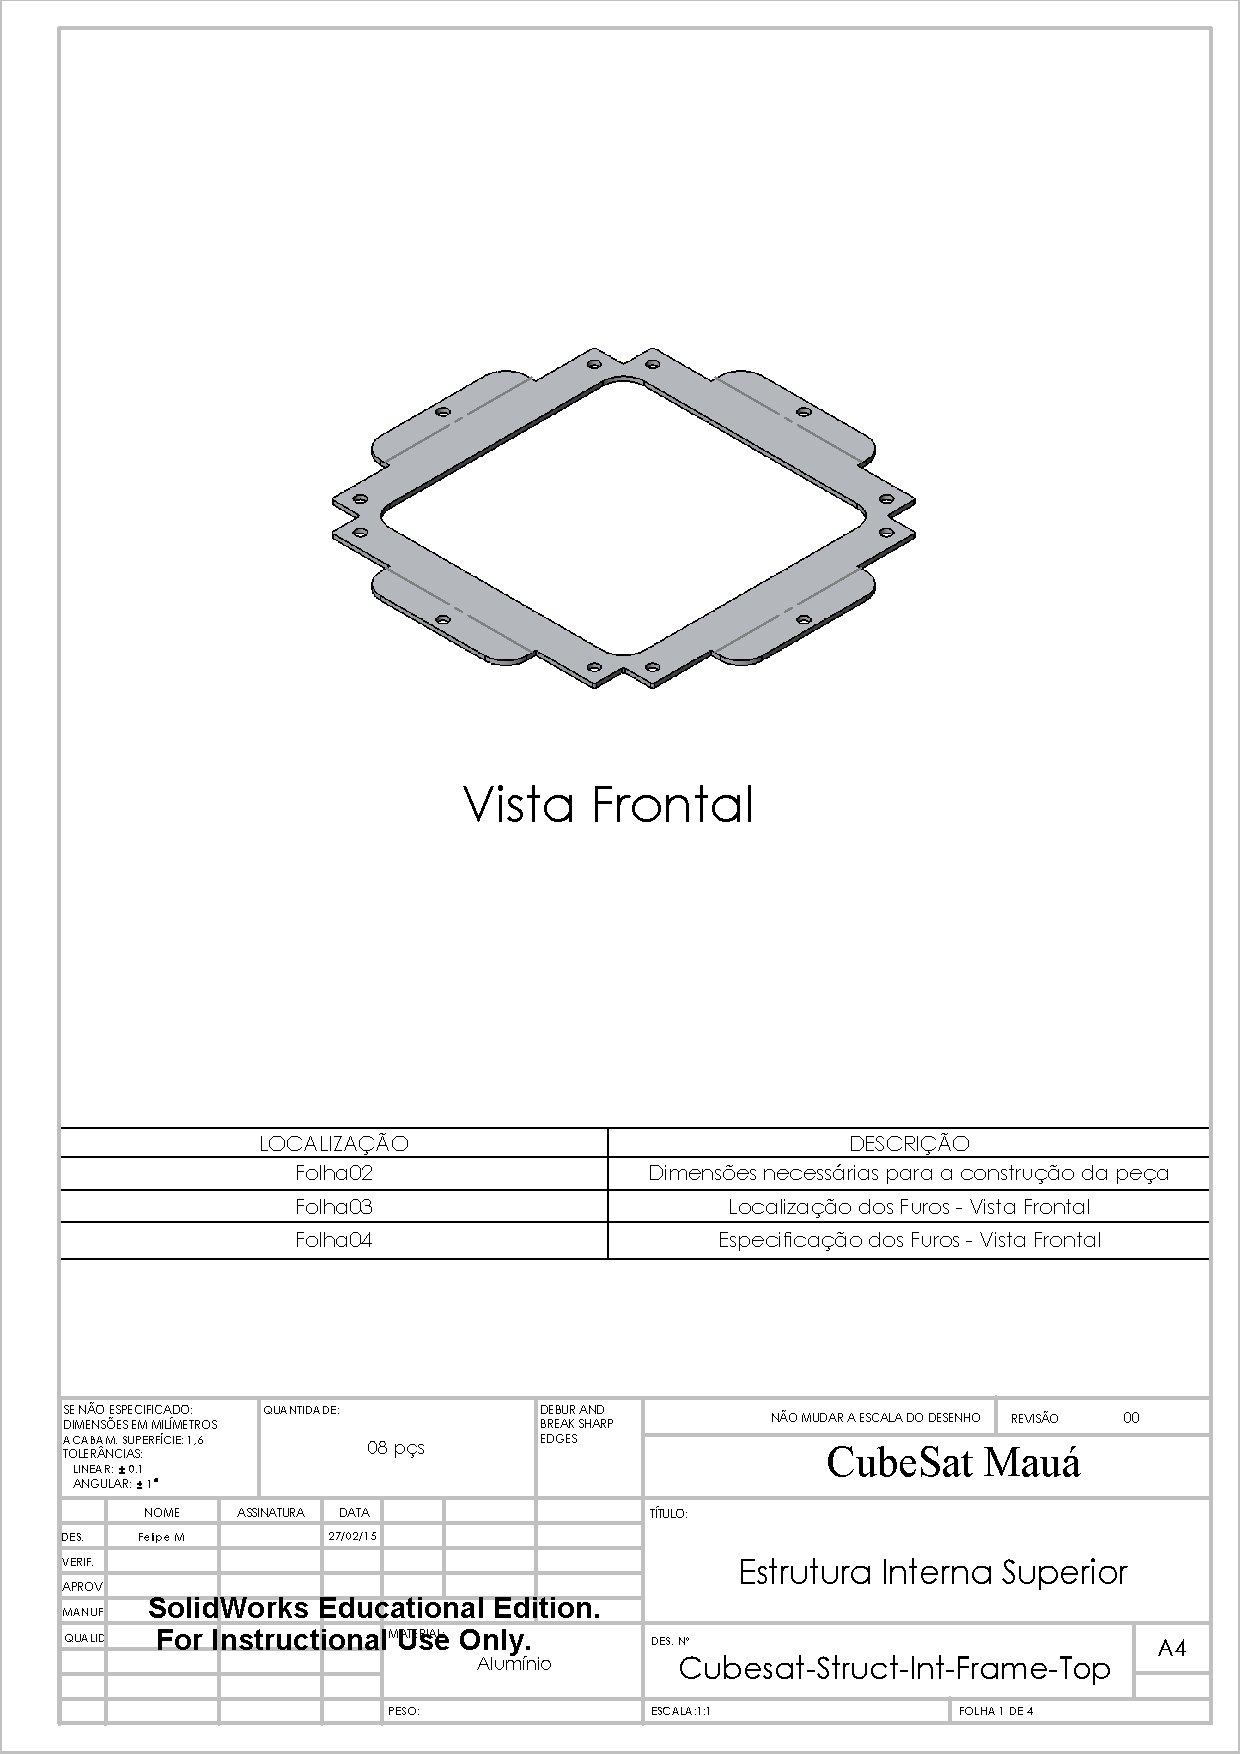
\includepdf[pages=-]{./pdfs/Cubesat-Struct-Int-Frame-Top}
%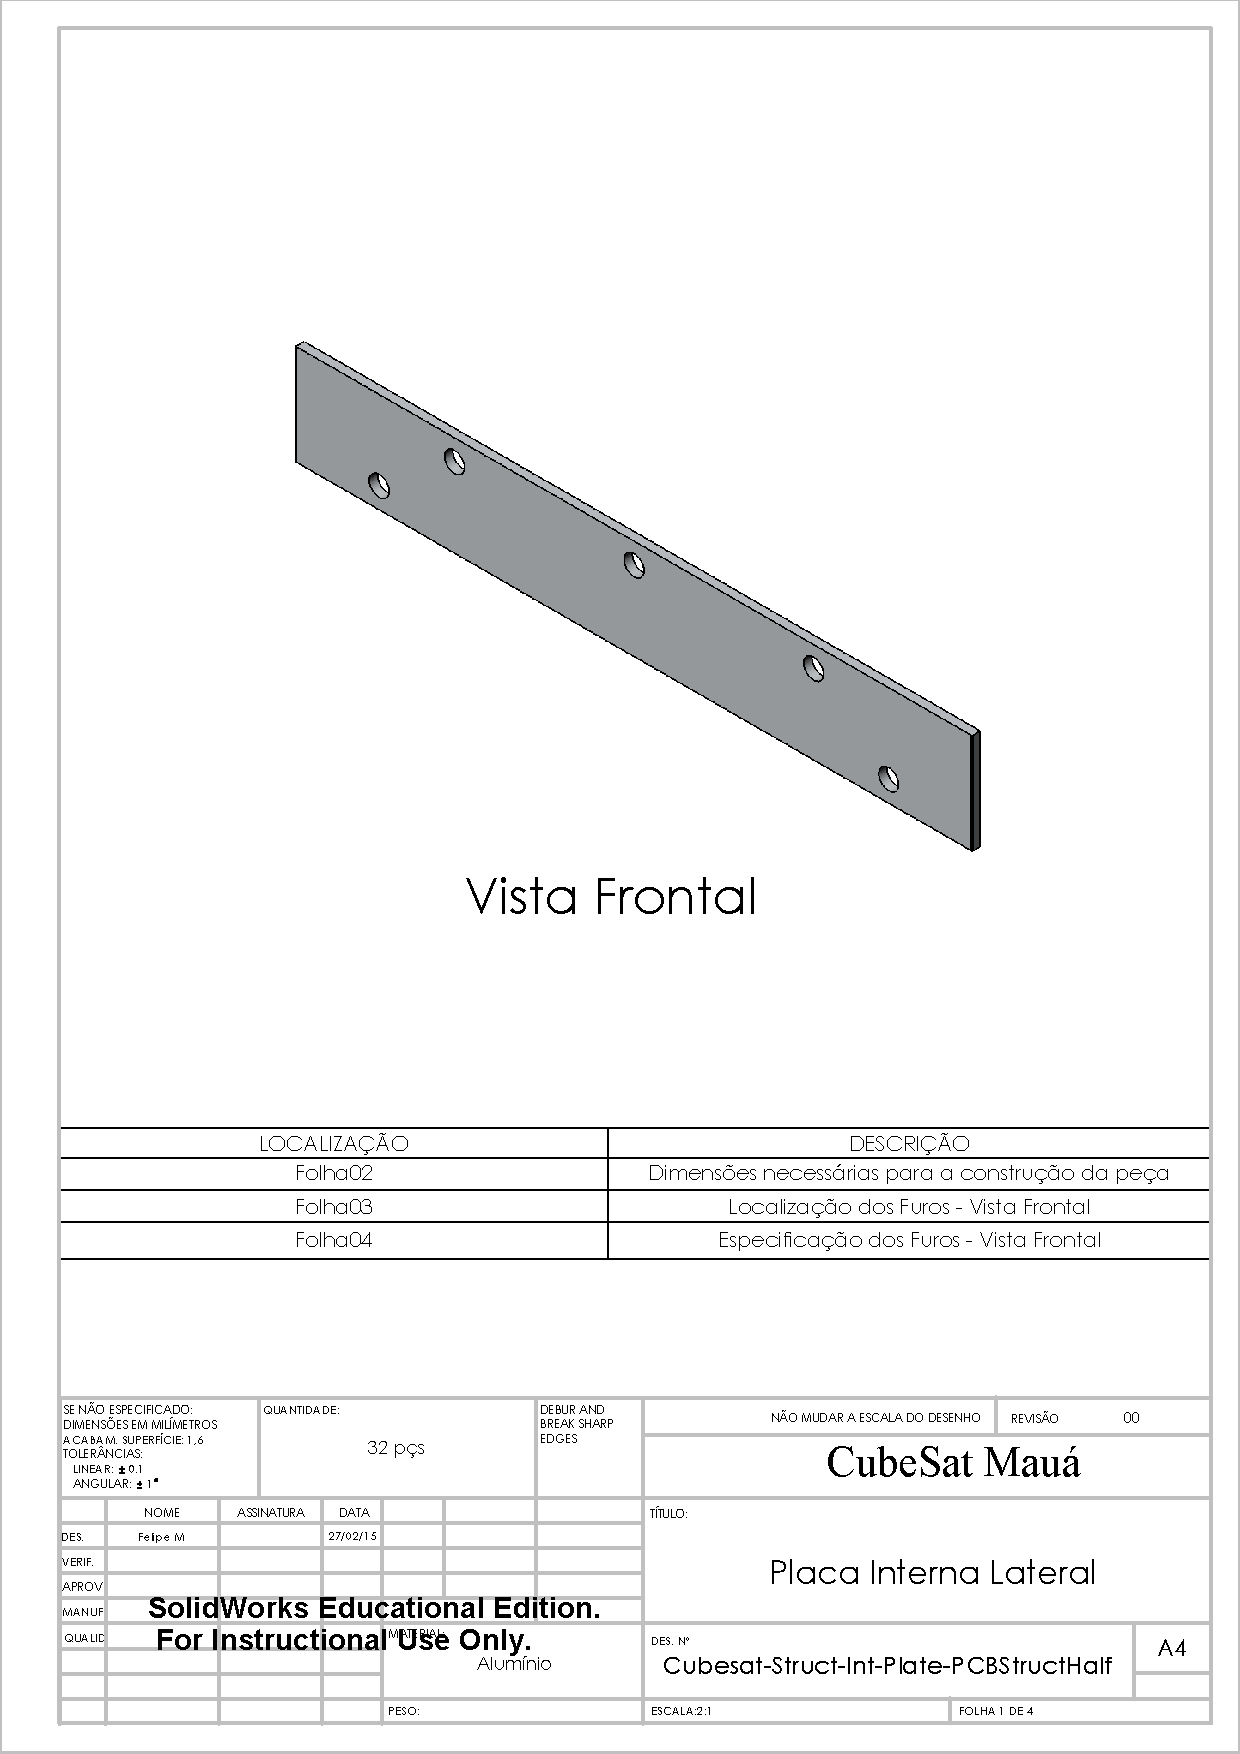
\includepdf[pages=-]{./pdfs/Cubesat-Struct-Int-Plate-PCBStructHalf}

\chapter{}

\label{an:}

\end{anexosenv}

\end{document}
